
\chapter{Introduction}
\label{chap:introduction}

Background -> problems -> motivation -> methods -> results\\

% Questions this work asks:\\
% 	How strong is the solar wind influence on the terrestrial magnetosphere?\\
% 	How often occur certain solar wind ranges?\\
% 	How strong do different structure types influence the terrestrial magnetosphere?\\
% forecast:\\
% 	How can the impact strength of the solar wind be forecasted? (VBz->Kp L1-Alerts)\\
% 	How can the impact strength of CMEs be forecasted (V->Kp correlation for CMEs)?\\
% 	(How can the impact field strength of CMEs be forecasted (V->B correlation for CMEs)?)\\

% 	How does the solar wind evolve on its way from the Sun?\\
% 	How do the different structures evolve on their way from the Sun?\\
% 	What are the properties of the solar wind near the Sun?\\
% 	(Where does the solar wind get accelerated?)\\
% 	(How does the solar wind get accelerated?)\\
% 	(How is this related to the coronal heating problem?)\\

% Kp estimate from sw
The abundance of modern technological systems that are sensitive to disturbances in the terrestrial mangetic field increases.\\
These include critical systems, such as ..., whose potential disruptions would not only have severe economical impacts but would affect human lives as well.\\
The disturbances in the terrestrial magnetic field (geomagnetic storms) are evoked by the field's interaction with streams of particles emitted by the Sun (solar wind).\\
Variations in some solar wind parameters lead to a direct response in geomagnetic activity.\\
This work aims to quantify this response for different solar wind forecast situations.\\
For when magnetic field and velocity information is available and for when only velocity information is available and it is known wether it is ambient solar wind or a CME event.\\

% PSP sw estimate from Helios
Open key questions are which mechanisms heat the corona and accelerate the solar wind.\\
The PSP mission is intended to clarify this.\\
As it is the first s/c to fly that near to the Sun, the solar wind environment is not known.\\
This is the motivation for the second part of this work.\\
This work derives estimates of that solar wind environment.\\

thesis goal: finding more precise relationships between parameters/quantities for being able to make better forecasts\\

catch from chapter abstracts...\\

This thesis presents quantitative analyses of the solar wind impact strengh on the terrestrial magnetosphere and of the estimated near-Sun solar wind environment.\\


%Synopsis	% Outline (chapters and their content)
I structured this work as follows: The fundamentals about the Sun, its activity, solar wind, and space weather are laid in \autoref{chap:basics}. The instrumentation and data sources used in this work are described in \autoref{chap:data}. The influences on the \Kp{}~index from solar activity, solar wind, CMEs, and solar wind streams are analyzed in \autoref{chap:chapter2}. In \autoref{chap:empirical_solar_wind_model_for_the_inner_heliosphere}, which is followed by the published paper on the same topic (integrated as \autoref{chap:solar_wind_predictions_for_the_parker_solar_probe_orbit}), an empirical solar wind model for the inner heliosphere is developed and used to estimate the near-Sun solar wind environment for the planned PSP mission. \autoref{chap:summary} summarizes the results and gives an outlook for further studies. Useful equations and information are located in the \autoref{chap:appendix}.



\chapter{Background knowledge}
\label{chap:basics}
%COFI -- chapter outline and flow integration
This chapter summarizes the basic knowledge necessary for understanding the analyses performed in this work. First, the Sun's origin, inner structure, atmosphere and heliosphere are described. Then, the Sun's dynamics with its differential rotation and magnetic field generation are outlined. Further, the solar activity cycle is described, including the meridional flow circulation, appearance of active regions, the surface magnetic field change, and sunspot cycles. The heliospheric magnetic field is pictured from its photospheric emergence in magnetic bright points and coronal superradial expansion, through the formation of the heliospheric current sheet and the Parker spiral to the heliosheath. The solar wind and its properties, the origins of slow and fast streams, stream interaction regions, and coronal mass ejections are described. Furthermore, space weather, solar influence on Earth, the magnetosphere, solar wind-magnetosphere coupling, and geomagnetic indices are portrayed.


\section{The Sun}
\label{sec:solar_composition}

%%% universe
13.8~billion years ago the Big~Bang formed our universe. The energy density of our universe consists of \SI{69.1}{\percent} dark energy, \SI{25.9}{\percent} dark matter and \SI{4.9}{\percent} baryonic matter, according to calculations using the inflationary $\Lambda$CDM\footnote{$\Lambda$CDM: Lambda cold dark matter} cosmology together with the latest cosmic microwave background temperature measurements \citep{Planck2016}.
%see Planck2016 page 31 Table 4		age of universe
%see Planck2016 page 31 Table 4 and en.wikipedia.org/wiki/Lambda-CDM_model#Parameters
%energy density consists of
%dark energy $\Omega_\Lambda = 0.6911$,
%matter $\Omega_\text{m} = 0.3089$,
%dark matter $\Omega_\text{c} = 0.2589$ and
%baryonic matter $\Omega_\text{b} = 0.0486$
After a few minutes the primordial nucleosynthesis left the universe in a state where the baryonic matter was composed of \SI{75.33}{\percent}\footnote{Percentages by mass.} hydrogen, \SI{24.67}{\percent} helium and traces of deuterium, tritium and lithium \citep{Planck2016}.
%see Planck2016 page 47 Eq. 73

%%% star formation
Over millions of years this gas cooled down and gravitationally accreted into molecular clouds and formed stars. The first generations of stars (Population~III) fused this gas to heavier elements (metals) and supernovae distributed them into space as a foundation for the formation of new stars of low and high metallicity (Population~II and I). Likewise, supernovae of these stars constantly enriched the interstellar medium with metals. Now, the interstellar medium in the Milky~Way consists of about \SI{32}{\percent} helium and traces of other metals \citep{Danziger1970}.
%In 20XX the Voyager~? probe measured a density of about ...\SI{0}{\per\cm\cubed} right outside of the heliopause (cite?).\\

%%% solar interior
Our Sun, a metal-rich Population~I yellow dwarf star, emerged 4.6~billion years ago \citep{Bahcall1995} from an accretion disk, formed by a collapsing rotating cloud. The compression within its center resulted in high temperatures, which initiated the fusion of hydrogen to helium (primarily pp~chain reaction). The fusion reactions produce huge amounts of energy and heat the solar center to a temperature of 15.7~million~kelvins \citep{Christensen-Dalsgaard1996}. The generated energy is transported through the solar body to its surface and eventually into space.
The core region extends to about 0.25~solar radii (\Rsun), where the declining temperature becomes insufficient for fusion reactions. The energy transport is dominated by thermal radiation until, because of declining ionization and density, at 0.71\,\Rsun{} up to the surface convective motion takes over \citep{Christensen-Dalsgaard1991}. %0.7: http://adsabs.harvard.edu/abs/1991ApJ...378..413C
%Dalsgaard Model S: http://astro.phys.au.dk/~jcd/solar_models/
%core radius (cite?)

%%% photoshere + sunspots
The temperature at this transition region, called tachocline, is about 2~million~kelvins and decreases up to the solar surface to between \SIrange{4400}{6600}{\K}\footnote{NASA Sun fact sheet: \urlfoot{https://nssdc.gsfc.nasa.gov/planetary/factsheet/sunfact.html}}. Here at the photosphere, the energy is radiated away with an effective black body temperature of \SI{5772}{\K} \citep{Mamajek2015}, classifying the Sun as a spectral type G2V star.
At this surface layer, granules, the tops of convection cells, and temporary sunspots are visible. Strong magnetic flux inhibits the convection at sunspots, leading to lower temperature and brightness (for more on sunspots see the following Sections~\ref{sec:solar_dynamo} and~\ref{sec:solar_activity_cycle}). \autoref{fig:sun_interior_HMIIC} illustrates these photospheric features along with the inner solar structure.
\begin{figure}[htb]
	\fcapside[\FBwidth]{
		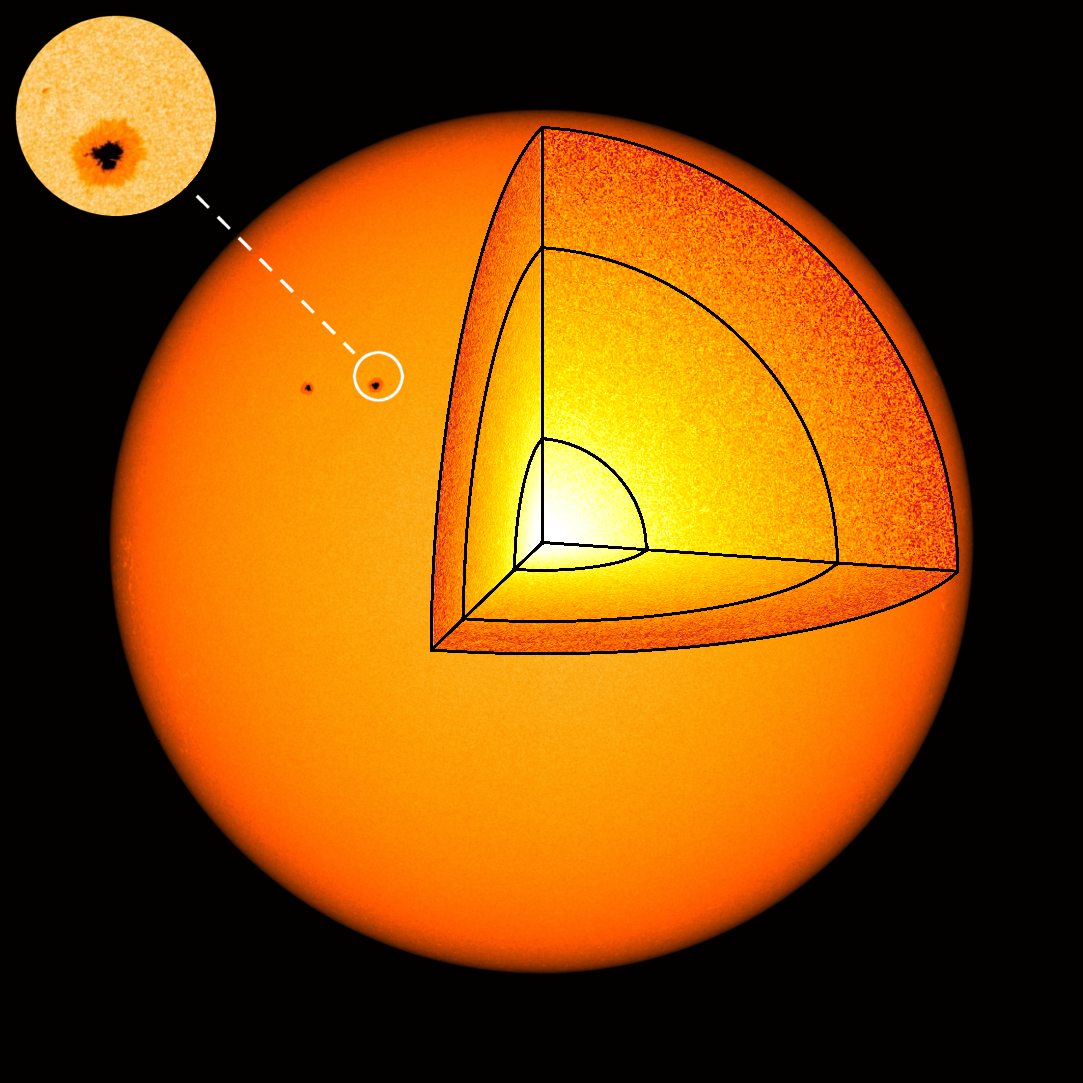
\includegraphics[width=0.6\textwidth]{figures_of_mine/schemata/sun_interior_HMIIC.png}
	}{
		\caption[\lofimage{figures_of_mine/schemata/sun_interior_HMIIC.png}I created this figure based on a SDO/HMI continuum image, credit: NASA/SDO and the AIA, EVE and HMI science teams.]
		{Image of the photosphere from 20~March~2016 together with a schema of the solar interior structure. The inset shows the granular surface with a sunspot. I created this figure based on a SDO/HMI continuum image, credit: NASA/SDO and the AIA, EVE and HMI science teams.}
		\label{fig:sun_interior_HMIIC}
	\addtocontents{lof}{\smallskip\protect\center I created the figure from NASA images.\medskip}
	}
\end{figure}

%%% chromosphere + corona + CMEs
Above the photosphere at the base of the chromosphere, the temperature declines to its solar minimum of \SI{3800}{\K} until it raises to \numrange{2}{3}~million~kelvins in the corona \citep{Billings1959,Liebenberg1975}. Up to now it is not fully understood why the corona is so much hotter than the underlying chromosphere -- this question is known as the coronal heating problem \citep{Klimchuk2006,McComas2007,Fox2015}. The generally considered energy transfer mechanisms are magnetic reconnections, wave heating and type~II spicules or a combination of these \citep{Cranmer2017}.

The chromosphere is a \SI{2000}{\km} thick region, whose features -- numerous spicules, filaments, and prominences -- can reach far into the corona. They consist of chromospheric material, channeled by the solar magnetic field, and are enveloped by a thin transition region where the temperature jumps up from about \SI{30000}{\K}\footnote{NASA Sun fact sheet: \urlfoot{https://nssdc.gsfc.nasa.gov/planetary/factsheet/sunfact.html}} to coronal temperatures. Reconnection of magnetic field lines can result in the eruption of filaments into the corona and beyond, termed coronal mass ejections (CMEs), see also \autoref{sec:coronal_mass_ejections}. Details of chromospheric features are shown in \autoref{fig:sun_atmosphere} -- the images were taken on the same day as in \autoref{fig:sun_interior_HMIIC}.
\begin{figure}[htb]
	\fcapside[\FBwidth]{
		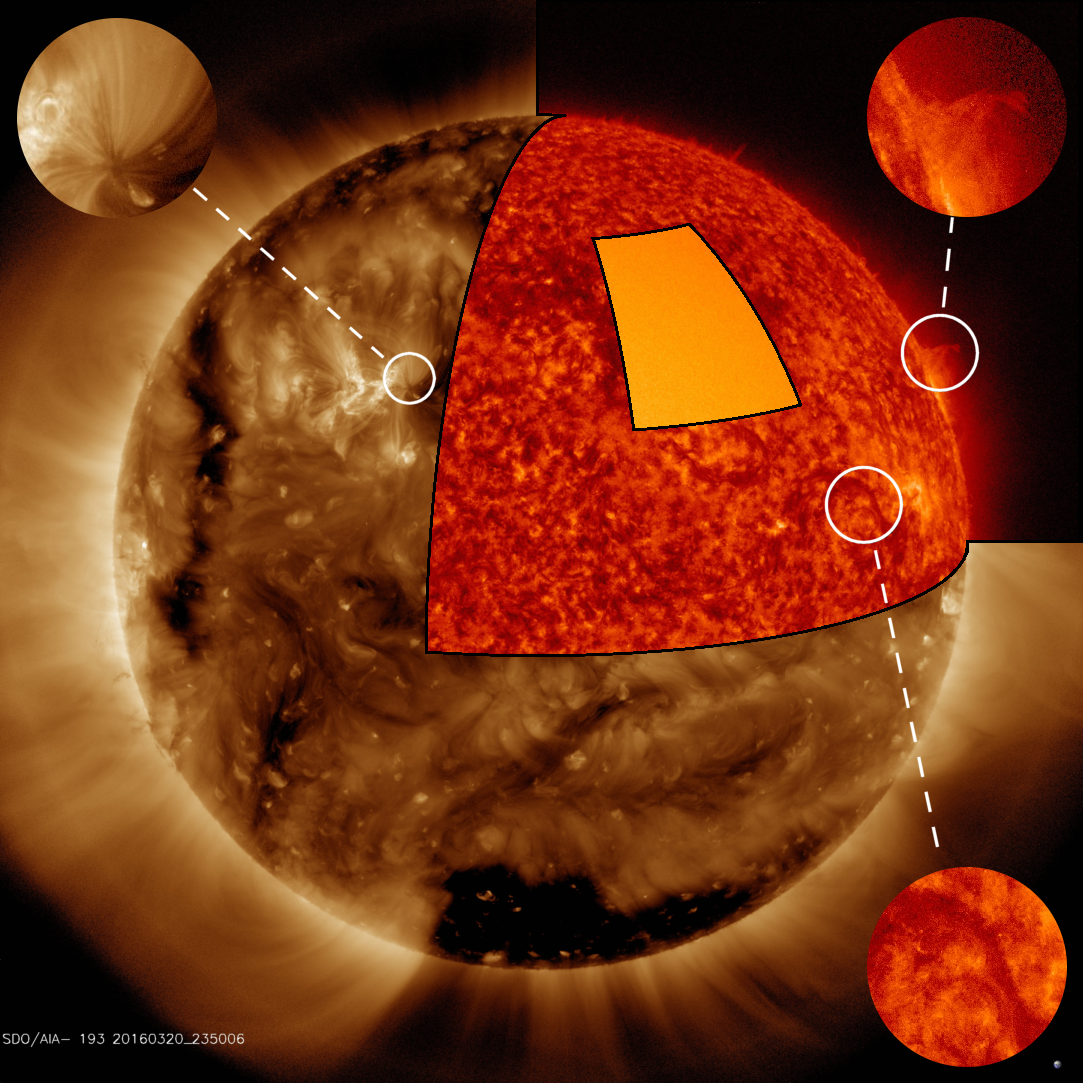
\includegraphics[width=0.6\textwidth]{figures_of_mine/schemata/sun_atmosphere.png}
	}{
		\caption[\lofimage{figures_of_mine/schemata/sun_atmosphere.png}I created this figure based on SDO/AIA images, credit: NASA/SDO and the AIA, EVE and HMI science teams.]
		{Composite image of the solar atmosphere from 20~March~2016 and some details of its features. Corona, chromosphere and photosphere are seen in wavelengths of \SI{193}{\angstrom}, \SI{304}{\angstrom}, and continuum. Chromospheric spicules are visible on the northern limb. The enlargements on the right show a prominence and a filament. The dark region at the south pole is a coronal hole. The left inset shows details of the active region belonging to the sunspots shown in \autoref{fig:sun_interior_HMIIC}. I created this figure based on SDO/AIA images, credit: NASA/SDO and the AIA, EVE and HMI science teams.}
		\label{fig:sun_atmosphere}
	}
	\addtocontents{lof}{\smallskip\protect\center I created the figure from NASA images.\medskip}
\end{figure}

%%% coronal holes
The Sun's atmosphere is dominated by the varying small- and large-scale solar magnetic field configuration. There are regions where the magnetic field lines arc back to the surface and regions with open field lines. In the latter areas the coronal plasma can -- guided by the field -- escape into space. Thus these coronal areas are less dense, cooler and therefore appear darker in extreme ultraviolet (EUV) and are called coronal holes (CHs). In \autoref{fig:sun_atmosphere} a coronal hole is visible at the solar south pole.

%%% corona
From Earth, the faint corona and chromosphere can only be observed during eclipses, because of the brightness of the solar disk. There are three effects contributing to the visibility of the corona: photons scattering off free electrons, producing a continuous spectrum; photons scattering off dust particles, their spectrum contains Fraunhofer absorption lines; and ion spectral emission lines -- these contributions to the corona are termed K-, F- and E"~corona\footnote{K from kontinuierlich (continuous in german), F from Fraunhofer, and E from emission.}.
% the so-called K-, F- and E"~corona (K kontinuierlich, F Fraunhofer, E emission).\\
% K-corona: photon scattering off free electrons --> coronagraphs\\
% F-corona: photon scattering off dust particles; contains Fraunhofer absorption lines; expands in ecliptic as zodiacal light --> coronagraphs\\
% E-corona: ion spectral emission lines; reveals coronal composition --> images\\
Images from solar eclipses reveal the coronal plasma, shaped by the magnetic field, and red prominences from the chromosphere. The solar eclipse imaged in \autoref{fig:Tse2008_500_mo1} shows the magnetic field's dipole structure and the equatorial streamer belt, characteristic for a quiet Sun during cycle minimum.
\begin{figure}[htb]
	\fcapside[\FBwidth]{
		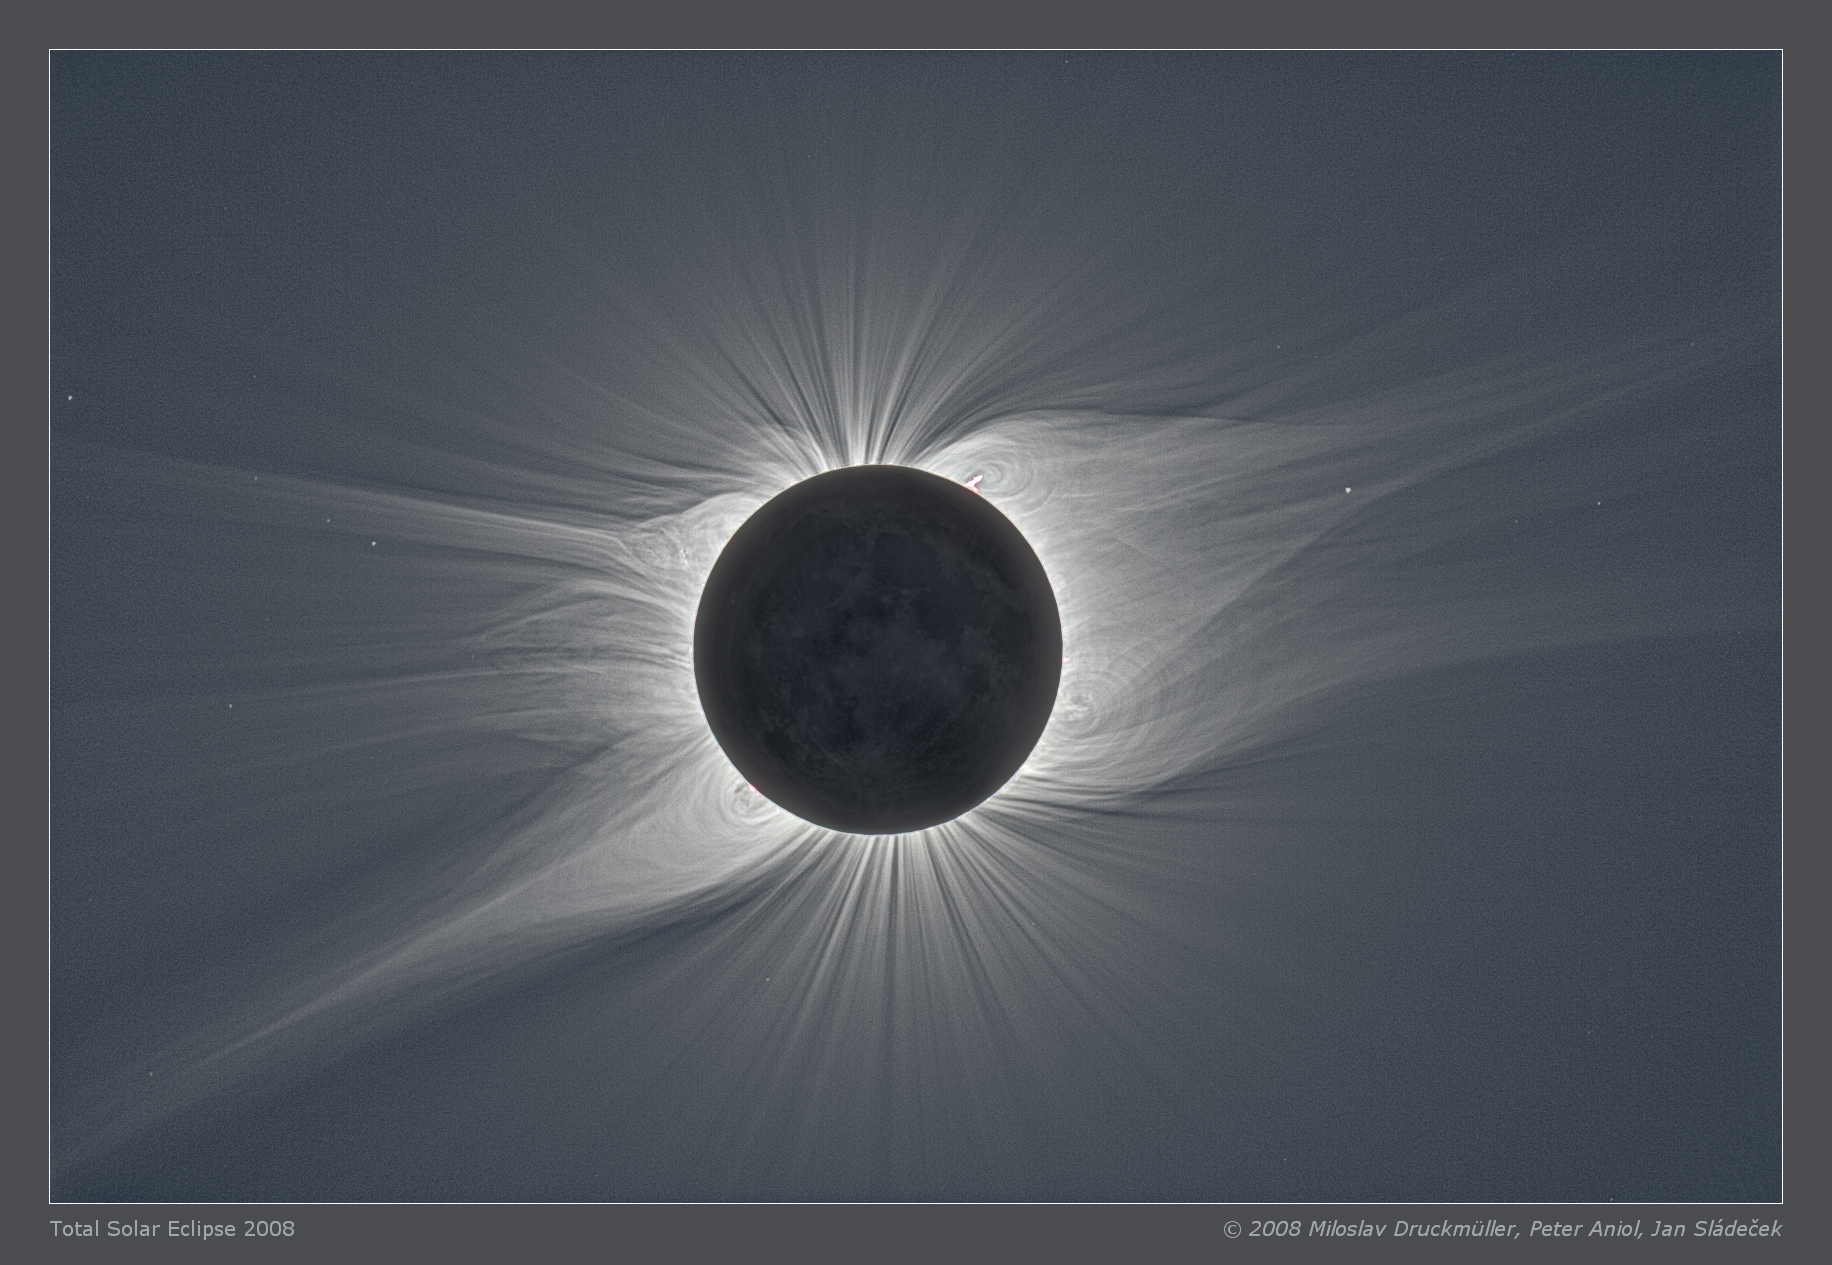
\includegraphics[width=0.6\textwidth]{figures_of_others/images/Tse2008_500_mo1.png}
	}{
		\caption[\lofimage{figures_of_others/images/Tse2008_500_mo1.png}Credit: \href{http://www.zam.fme.vutbr.cz/~druck/Eclipse/}{Miloslav Druckmüller, Peter Aniol, Jan Sládeček}, 2008, reproduced with permission.]
		{Total solar eclipse image of the inner corona up to a distance of five solar radii. The picture was taken in Mongolia, 1~August~2008 and is processed from multiple images. Credit: \href{http://www.zam.fme.vutbr.cz/~druck/Eclipse/}{Miloslav Druckmüller, Peter Aniol, Jan Sládeček}, 2008, reproduced with permission.}
		\label{fig:Tse2008_500_mo1}
	}
	\addtocontents{lof}{\smallskip\protect\center See the following email correspondence.
		\protect\lstinputlisting{figures_of_others/permissions/Druckmuller_permission.txt}\medskip
	}
\end{figure}
%figure source: http://www.zam.fme.vutbr.cz/~druck/Eclipse/Ecl2008m/Tse2008_500_mo1/Hr/Tse2008_500_mo1.png

%%% solar wind + heliosphere
Due to the high coronal temperatures, plasma escapes the solar gravitational field \citep{Parker1958} with velocities of \SIrange{200}{800}{\km\per\s}. Its acceleration is linked to the coronal heating -- however, the exact location and process remain an open question \citep{Hollweg1985,McComas2007,Fox2015,Cranmer2017}. The magnetic field becomes too weak to guide the coronal plasma at a distance of a few solar radii. From this so-called source surface, the solar wind flows radially outward into space until it reaches the termination shock. Eventually it collides with the local interstellar medium, creating the boundary of the heliosphere, the heliopause. The heliopause is expected to be a bubble of either teardrop or croissant shape, caused by the Sun's relative velocity of \SI{23}{\km\per\s} with respect to the local interstellar medium \citep{Owens2013, Opher2015}. Thus, there may exist a leading bow shock. Measurements of the Voyager~1 and 2 spacecraft indicate their passage of the termination shock at about \SI{94}{\au} and \SI{84}{\au}, entering the heliosheath region \citep{Owens2013}. \citet{Gurnett2013} report that in 2012 Voyager~1 actually crossed the heliopause into interstellar space at a solar distance of \SI{121}{\au}. The heliosphere and its surrounding flow structure is illustrated in \autoref{fig:Owens2013_Heliosphere_screenshot}.
\begin{figure}[htb]
	\fcapside[\FBwidth]{
		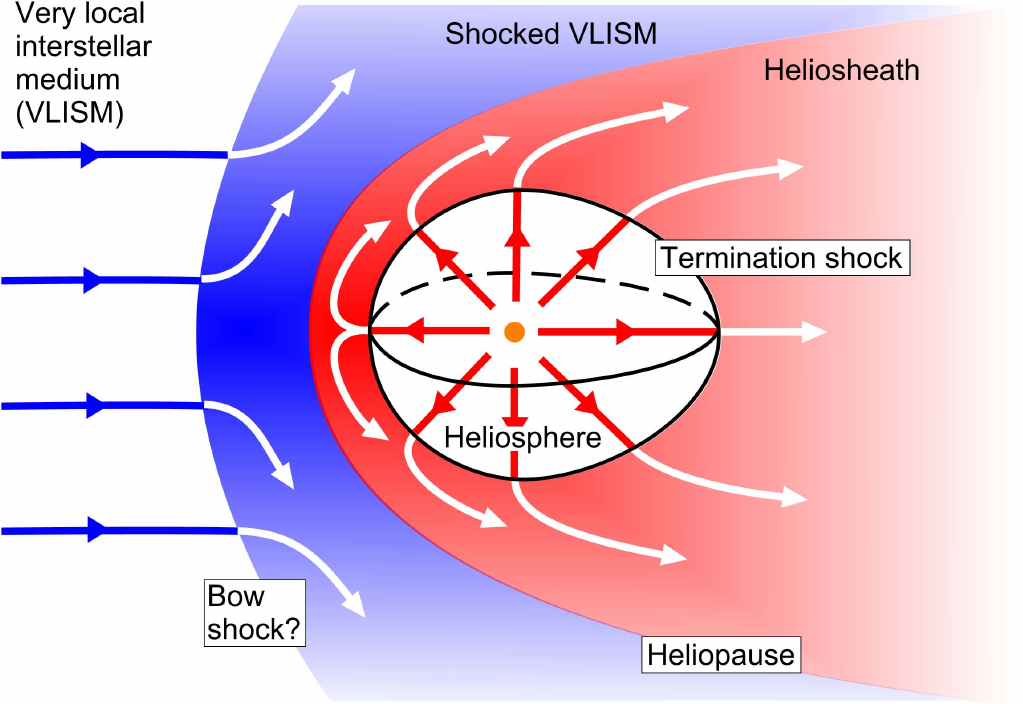
\includegraphics[width=0.6\textwidth]{figures_of_others/images/Owens2013_Heliosphere_screenshot.png}
	}{
		\caption[\lofimage{figures_of_others/images/Owens2013_Heliosphere_screenshot.png}Credit: {\citet[Fig.~9]{Owens2013}}, licensed under \href{https://creativecommons.org/licenses/by-nc/3.0/de/}{CC BY-NC 3.0 DE}.]
		{Schema of the heliosphere and its surrounding flow structure, formed by the interaction of the solar wind (red) with the local interstellar medium (blue) at the heliopause. Credit: {\citet[Fig.~9]{Owens2013}}, licensed under \href{https://creativecommons.org/licenses/by-nc/3.0/de/}{CC BY-NC 3.0 DE}.}
		\label{fig:Owens2013_Heliosphere_screenshot}
	}
	\addtocontents{lof}{\smallskip\protect\center See the following RightsLink request result.\protect\\
		\protect\fbox{\protect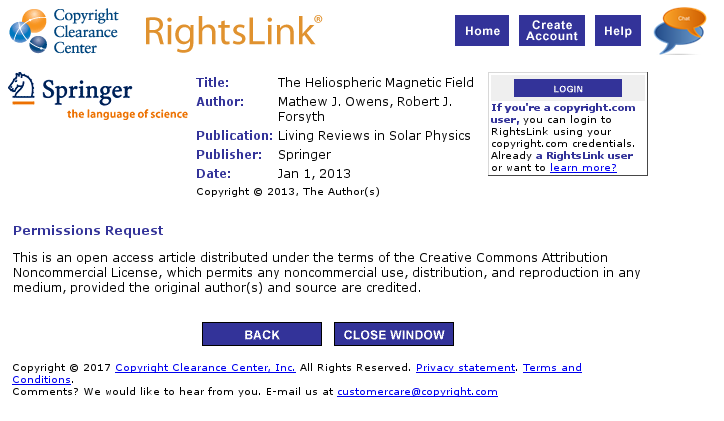
\includegraphics[width=0.7\textwidth]{figures_of_others/permissions/permission_request_Owens2013.png}}\protect\\
		\medskip
	}
\end{figure}
%Owens2013 figure permission request: open access article

%%% solar wind influence + space weather
On its way outwards through the solar system, the solar wind -- carrying the solar magnetic field -- interacts with the planets, their magnetic fields and other solar system bodies. This has various effects, for instance disturbances in planetary magnetic fields with appearance of aurorae and enhanced radiation, atmospheric losses and stripping of cometary tails. Some of these effects can have disruptive consequences for humans and their technology, creating a high interest in understanding space weather and forecasting its effects, the topic of space weather is further addressed in \autoref{sec:space_weather}. The magnitudes of these effects depend highly on spatial and temporal variations in the solar wind, which are rooted in the dynamics of the solar magnetic field, described in the following sections.

%%%%%%%%%%%%%%%%%%%%%%%%%%%%%
%\section{Stars/Beginning}
% introduction leading to stars; beginning from universe/big bang\\
% gravitational contraction of rotating nebula\\
% -> fusion burning; energy production\\
% In its core it fuses hydrogen to helium; 15.7~million~K; inner 25~\%\\
% energy transport -> radiation zone; up to 70~\%\\
% tachocline ~2~million~K\\
% energy transport by convection -> convection zone; up to surface\\
% convective granulation\\
% photoshere 4400--6600~K, effective black body temperature 5777~K; spectral class\\
% (herzsprung russell diagram)\\
% chromosphere... (solar atmosphere figure)\\
% transition region\\
%corona 1--3~million~K temperature (coronal heating problem)\\
% coronal holes: open magnetic field lines, solar wind\\
% heliosphere, shock with interstellar medium (ISM); Voyager\\

%%%%%%%%%%%%%%%%%%%%%%%%%%%%%
%big bang
%to formation of stars
%to ISM in our galaxy
%to formation of Sun
%Sun's inner structure (energy production and transport)
%its surface (radiation, spectral class)
%its outer structure (chromosphere, corona, solar wind, heliosphere)
%its heliosphere (termination shock with ISM, Voyager measurements)
%%%%%%%%%%%%%%%%%%%%%%%%%%%%%


\section{Solar dynamo}
\label{sec:solar_dynamo}
%%% differential rotation + solar magnetic field origin
The conservation of the angular momentum in the contracting molecular cloud led to a rotation of the Sun. Although the Sun experiences loss of angular momentum due to solar wind \citep{Weber1967}, its rotation still has a current average period of about 25~days. The radial convective motion within the solar interior above the tachocline leads to a transport of momentum away from the rotation axis and therefore to a slower polar and faster equatorial rotation in the convection zone \citep{Miesch2005}. This differential rotation is visible on the surface and was first discovered from sunspot observations by \citet{Scheiner1630}. With a rotation period of about 34~days, the poles have a lag of almost 9~days (for further information on solar rotation see appendix \autoref{sec:solar_surface_differential_rotation}). The differential rotation in the solar interior can be inferred from helioseismological observations. Below the differential rotation of the convection zone, a nearly solid rotation with a period of about \SI{26.6}{days} (this corresponds to a frequency of \SI{435}{\nano\hertz}) exists in the radiation zone, as shown in \autoref{fig:Miesch2005_fig1a_interior_diff_rot}.
\begin{figure}[htb]
	\begin{floatrow}
		\ffigbox{
			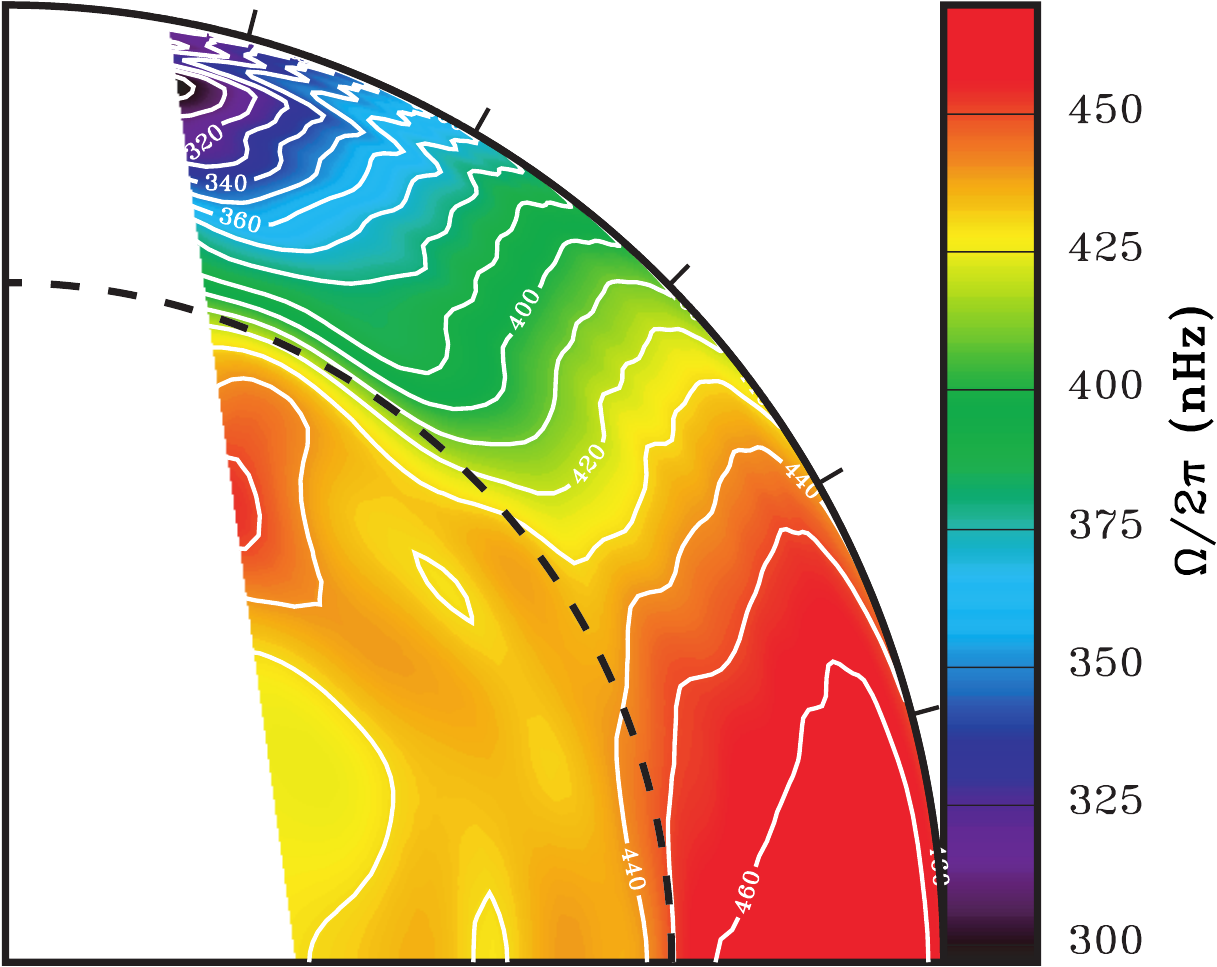
\includegraphics[width=0.5\textwidth]{figures_of_others/images/Miesch2005_fig1a_interior_diff_rot.png}
		}{
			\caption[\lofimage{figures_of_others/images/Miesch2005_fig1a_interior_diff_rot.png}Credit: {\citet[Fig.~3]{Thompson2003}}, \textcopyright~Annual~Reviews, reproduced with permission.]
			{Rotation frequency profile of the solar interior. The location of the tachocline is indicated by the dashed line. The rotation frequency is inferred from helioseismology via observations from the Michelson Doppler Imager (MDI) at the Solar and Heliospheric Observatory (SOHO) spacecraft. Credit: {\citet[Fig.~3]{Thompson2003}}, \textcopyright~Annual~Reviews, reproduced with permission.}
			\label{fig:Miesch2005_fig1a_interior_diff_rot}
			%(\citet[Fig.~1\,a]{Miesch2005}; based on \citet[Fig.~3]{Thompson2003})
			%Thompson2003 permission request: permission not required
		}
		\addtocontents{lof}{\smallskip\protect\center See the following RightsLink request result.\protect\\
			\protect\fbox{\protect
\includegraphics[width=0.7\textwidth]{figures_of_others/permissions/permission_request_Thompson2003.png}}\protect\\
			\bigskip
		}
		\ffigbox{
			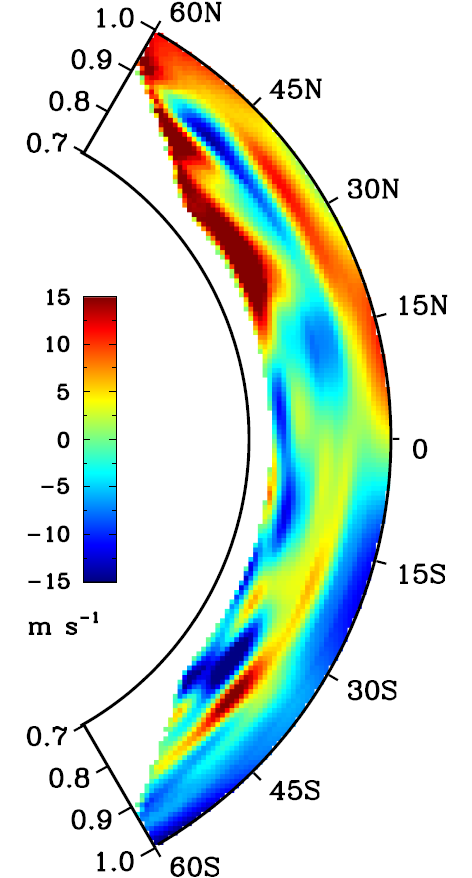
\includegraphics[width=0.28\textwidth]{figures_of_others/images/Zhao2013_meridional_flow.png}
		}{
			\caption[\lofimage{figures_of_others/images/Zhao2013_meridional_flow.png}Credit: {\citet[Fig.~4, panel~(a), I moved the colorbox]{Zhao2013}}, \textcopyright~AAS, reproduced with permission.]
			{Meridional flow velocity profile in part of the convection zone. Positive values are directed towards north. The velocity is inferred from helioseismology via observations from the Helioseismic Magnetic Imager (HMI) at the Solar Dynamics Observatory (SDO) spacecraft. Credit: {\citet[Fig.~4, panel~(a), I moved the colorbox]{Zhao2013}}, \textcopyright~AAS, reproduced with permission.}
			\label{fig:Zhao2013_meridional_flow}
			%Zhao2013 permission request: permission granted.
		}
		\addtocontents{lof}{\smallskip\protect\center See the following email correspondence.
			\protect\lstinputlisting{figures_of_others/permissions/Zhao2013_permission.txt}\medskip
		}
	\end{floatrow}
\end{figure}
%Angular velocity profile in the solar interior inferred from helioseismology (after Thompson et al., 2003). In panel (a), a 2D (latitude-radius) rotational inversion is shown based on the subtractive optimally localized averaging (SOLA) technique. All inversions are based on data from the Michelson Doppler Imager (MDI) instrument aboard the SOHO spacecraft, averaged over 144 days. Inversions become unreliable close to the rotation axis, represented by white areas in panel (a). Note also that global modes are only sensitive to the rotation component which is symmetric about the equator (courtesy M.J. Thompson \& J. Christensen-Dalsgaard).

%%% magnetic field dynamo mechanism
Turbulent plasma motions from convective flows in the convection zone generate and carry disorganized magnetic flux. The large rotational shear at the tachocline stretches and amplifies the magnetic fields to strong coherent toroidal flux ($\omega$-effect) with intensities of the order \SIrange{1}{10}{\tesla}. These toroidal fields, generated near the bottom of the convection zone, can be stored in a deep magnetic layer located in the stably stratified region below the convection zone \citep{Ossendrijver2003}. The stronger flux ropes become buoyant and raise to the surface. The Coriolis force twists them systematically on their way through the convection zone ($\alpha$-effect). The twist is stronger at higher latitudes (Joy's law). The flux ropes emerge then in the photosphere as bipolar active regions of opposite magnetic polarity -- the stronger ones forming pairs of sunspots, as seen in \autoref{fig:bipolar_region_HMIB_HMIIF}.
\begin{figure}[htb]
	\centering
	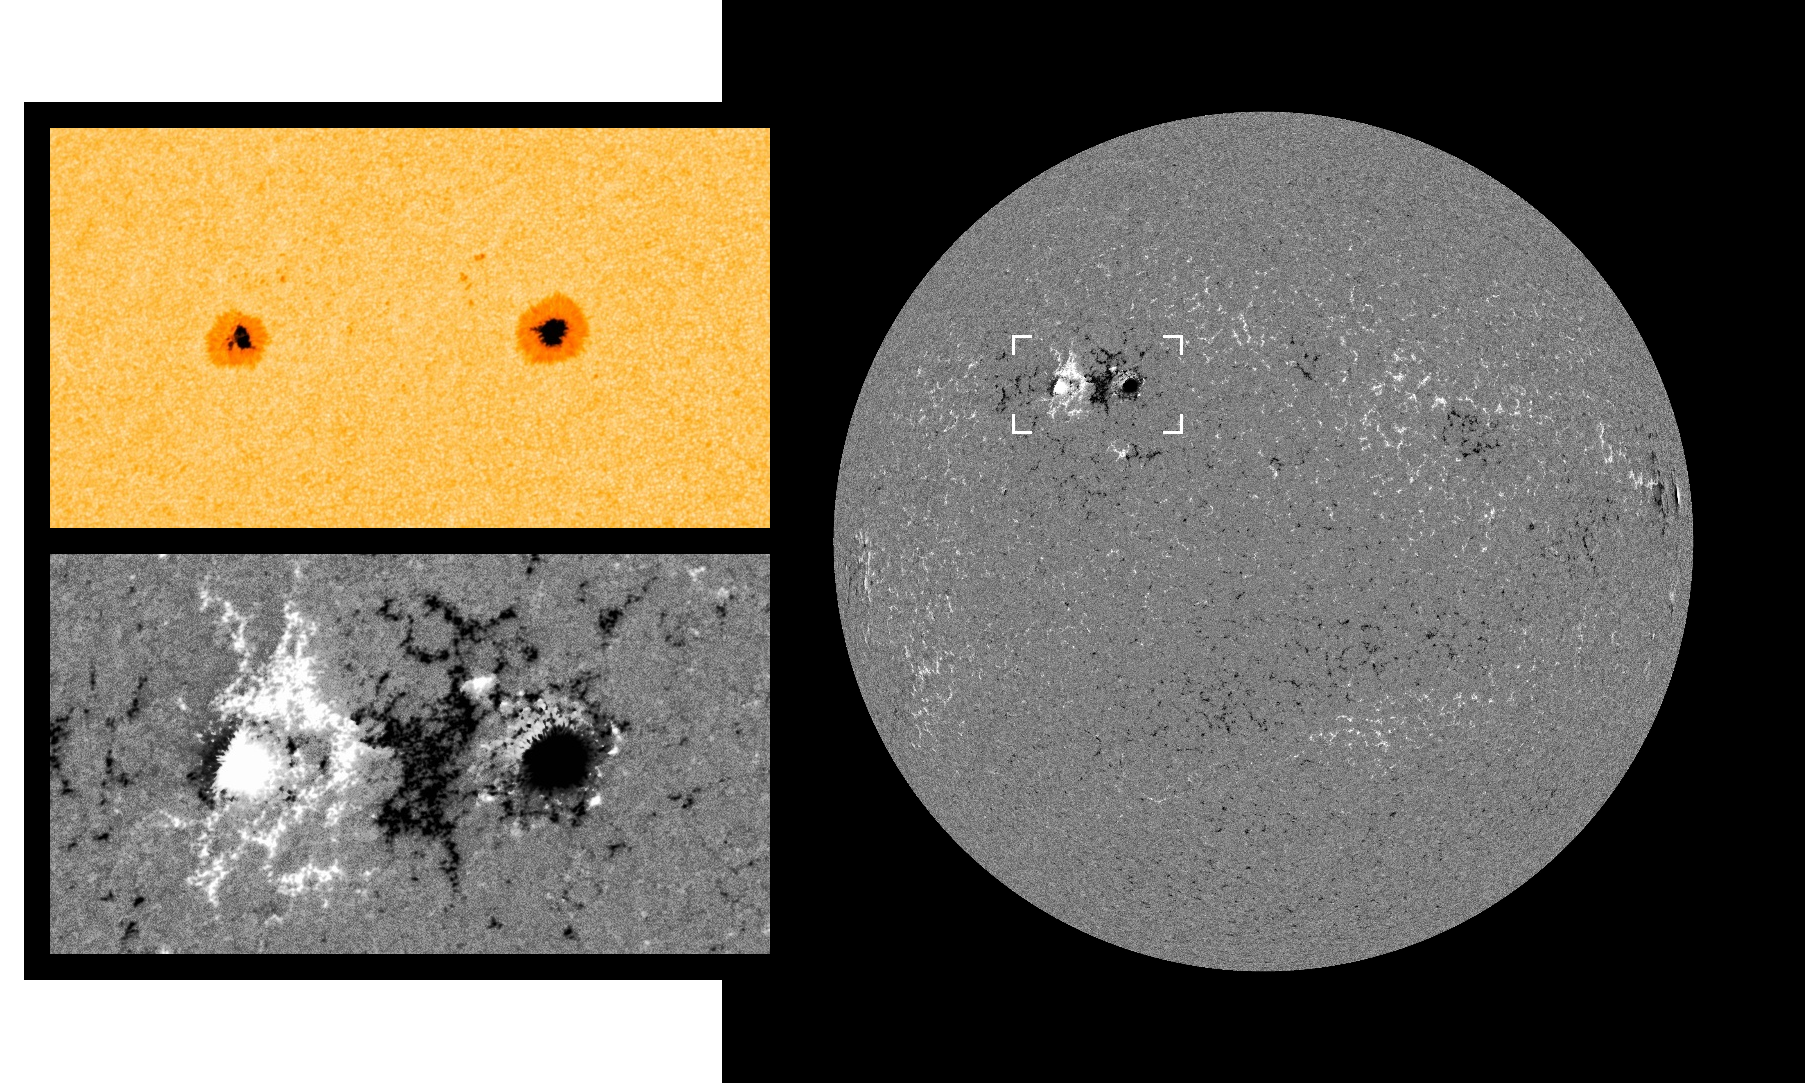
\includegraphics[width=\textwidth]{figures_of_mine/schemata/bipolar_region_HMIB_HMIIF.png}
	\caption[\lofimage{figures_of_mine/schemata/bipolar_region_HMIB_HMIIF.png}I created the figure based on SDO/HMI continuum and magnetogram images from 20~March~2016, credit: NASA/SDO and the AIA, EVE and HMI science teams.]
	{Continuum image of the two sunspots pictured in \autoref{fig:sun_interior_HMIIC} (top left), magnetogram from the same region (bottom left), and magnetogram from the whole solar disk (right). The magnetogram shows the polarity of the line-of-sight magnetic field component at the photosphere (black/white: inward/outward polarity). The highly concentrated magnetic flux at the sunspots is visible as well as the extended bipolar magnetic field structure of the whole active region, which is divided by the so-called magnetic neutral line. The solar disk is scaled to the same size as in \autoref{fig:sun_interior_HMIIC}. I created the figure based on SDO/HMI continuum and magnetogram images from 20~March~2016, credit: NASA/SDO and the AIA, EVE and HMI science teams.}
	\label{fig:bipolar_region_HMIB_HMIIF}
	\addtocontents{lof}{\smallskip\protect\center I created the figure from NASA images.\medskip}
\end{figure}
% HMI is a vector magnetogram, but the public sources say that the magnetogram shows a line-of-sight magnetic field.
Turbulent convective diffusion of this surface flux contributes to the build-up of poloidal fields. Their resulting polarity is opposite to the prevailing global field due to the directional way the rotational shear at the tachocline and the Coriolis force in the convection zone act. Fluctuating motions further amplify the mean fields in these processes. This solar $\alpha$-$\omega$-dynamo is thought to create the major part of the solar magnetic field. Still, with regard to the magnetic field's high variability, the long-term mean fields are governed by intermittent localized structures, that is, active regions, filaments and coronal loops \citep{Miesch2005}.	%Miesch2005 p.~18 + p.~31

% the $\alpha$-$\omega$-dynamo, see \autoref{fig:EOSFIG2_modified}\\
% \begin{figure}[htb]
% 	%\centering
% 	\fcapside[\FBwidth]{
% 		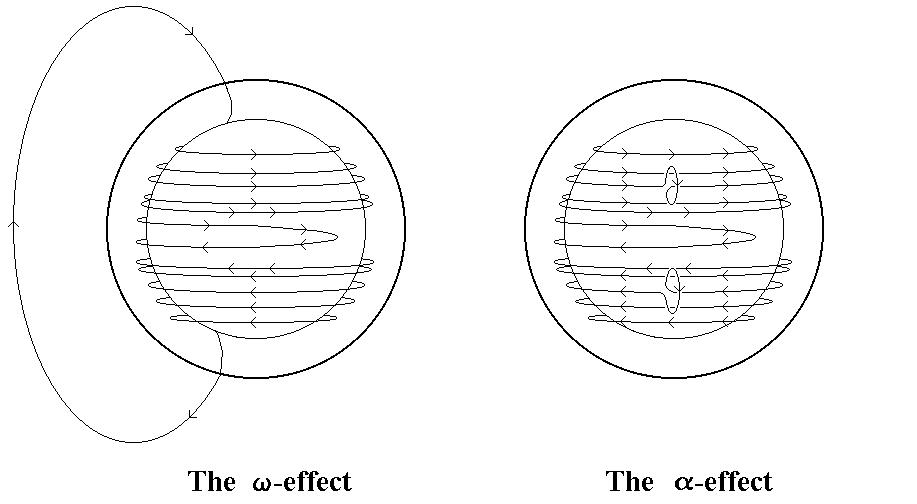
\includegraphics[width=0.5\textwidth]{figures_of_others/images/EOSFIG2_modified.png}
% 	}{
% 		\caption{Schemata of the $\omega$ and the $\alpha$-effects. figure really necessary? get permission...}
% 		\label{fig:EOSFIG2_modified}
% 	}
% \end{figure}
%http://certificate.ulo.ucl.ac.uk/modules/year_one/NASA_MSFC/solar_physics/dynamo.htm
%https://solarscience.msfc.nasa.gov/images/EOSFIG2.GIF

% switching between states of strong poloidal and toroidal field\\
% poloidal field + diff. rot. => toroidal field ($\Omega$-effect)\\
% the solar dynamo: (toroidal to poloidal field)\\
% - turbulent plasma motions from convective flows generate disorganized magnetic fields\\
% - differential shear at tachocline amplifies fields to strong coherent toroidal flux ($\Omega$-effect); magnetic layer located at the base of the convection zone\\
% - stronger flux ropes raise to surface (buoyantly)\\
% - Coriolis force twists them systematically, stronger at higher latitudes\\
% - twisted tubes emerge on the surface as bipolar active regions\\
% - amplification of mean fields by fluctuating motions ($\alpha$-effect) and turbulent diffusion create large-scale poloidal field\\


\section{Solar activity cycle}
\label{sec:solar_activity_cycle}
%%% convection cycle + solar surface magnetic field + solar cycle
Helioseismic measurements reveal that the large-scale convective flow is aggregated into large convection cells with slow meridional flows of a few \si{\m\per\s}, as can be seen in \autoref{fig:Zhao2013_meridional_flow}. A poleward subsurface flow and equatorward backflow beneath with a further poleward flow below are detected within each hemisphere, comprising a stacked double-cell profile \citep{Zhao2013}. The meridional circulation flow speed has a major influence on the average 22-year period of the emerging magnetic flux at the solar surface. This period varies and is influenced by the stochastic emergence rate and tilts of active regions and the diffusion from random convective motions \citep{Hathaway2016}. The surface magnetic field configuration changes within one period from a dipole structure to a reversed dipole structure with opposite polarity and back, completing a so-called Babcock-Leighton dynamo cycle. Thus, the transition time from one dipole state to the next lasts about 11~years, this period is defined as one solar cycle.
%http://www.solarcyclescience.com/forum/viewforum.php?f=9

%%% butterfly pattern
In the transition phase, magnetic flux emerges in belts above and below the solar equator, manifesting as bipolar active regions with sunspots, resulting in a toroidal/multipolar structured magnetic field. Sunspots appear at about \SI{+-20}{\degree} latitude at the beginning of a cycle, this shifts towards lower latitudes at the end of a cycle. Thus the plot of sunspots over latitude and time reveals a butterfly pattern \citep{Maunder1904}. This butterfly pattern appears in surface radial magnetic field observations as well, see \autoref{fig:Hathaway_magbfly}.
\begin{figure}[htb]
	\centering
	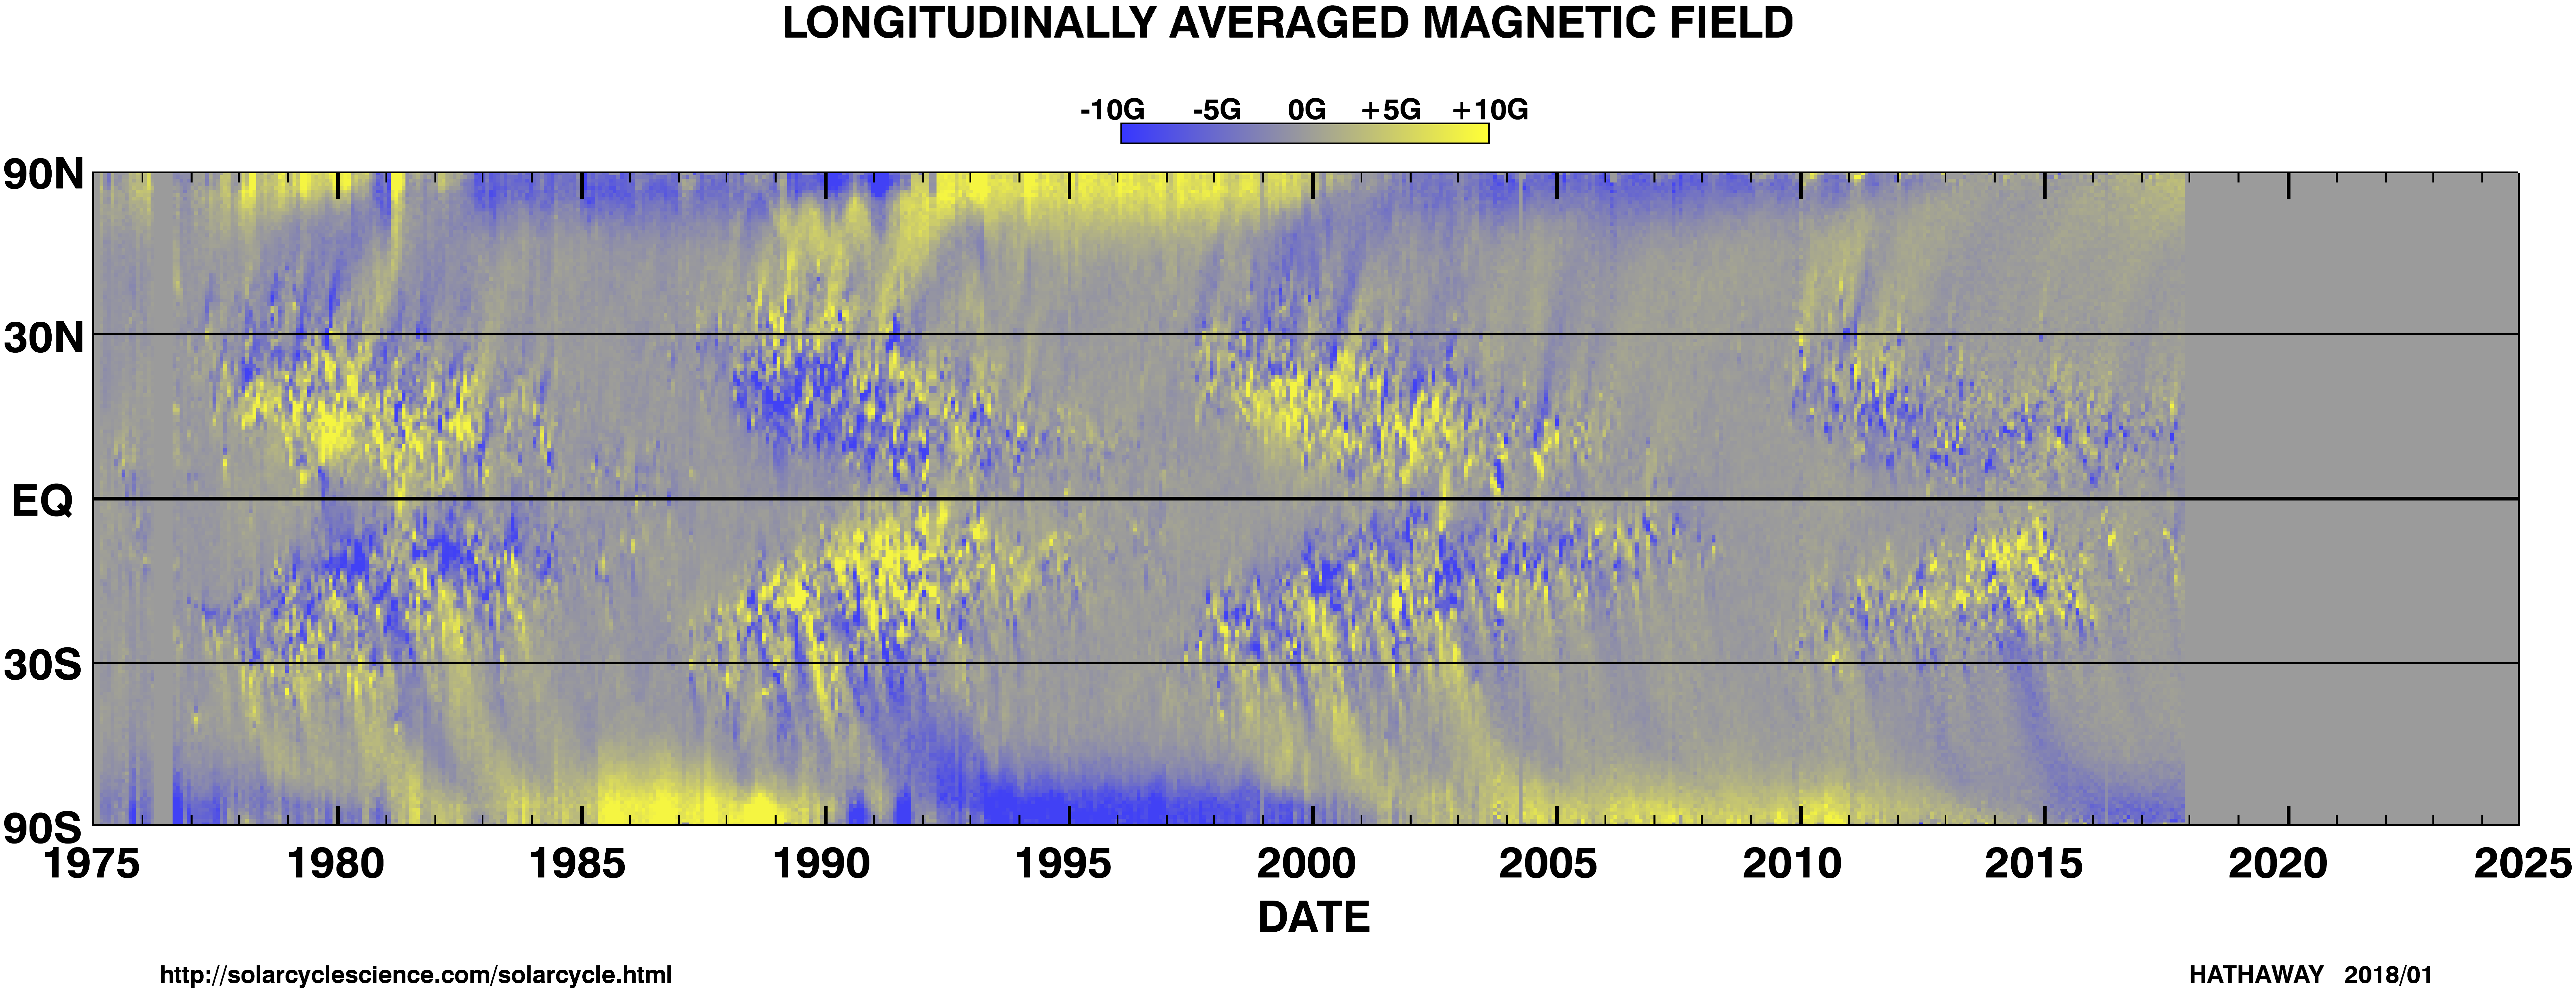
\includegraphics[width=\textwidth]{figures_of_others/images/Hathaway_magbfly_201801_cropped.png}
	\caption[\lofimage{figures_of_others/images/Hathaway_magbfly_201801_cropped.png}Courtesy of David~Hathaway, \href{http://solarcyclescience.com/solarcycle.html}{Solar Cycle Science}, 2018, updated version of {\citet[Fig.~17]{Hathaway2015}}.]
	{Magnetic butterfly diagram of the longitudinally averaged radial magnetic field on the solar surface. Yellow represents an outward directed magnetic field (positive), blue inward (negative). The data is obtained from instruments on Kitt~Peak National Observatory and from the MDI at the SOHO spacecraft. Courtesy of David~Hathaway, \href{http://solarcyclescience.com/solarcycle.html}{Solar Cycle Science}, 2018, updated version of \citet[Fig.~17]{Hathaway2015}.}
	\label{fig:Hathaway_magbfly}
	\addtocontents{lof}{\smallskip\protect\center See the following email correspondence.\medskip
		\protect\lstinputlisting{figures_of_others/permissions/Hathaway_permission.txt}
	}
\end{figure}
%Hathaway 2015 permission request: open access article
%figure source:	http://solarscience.msfc.nasa.gov/images/magbfly.jpg
%Hathaway website permission request: requested
%figure source:	http://solarcyclescience.com/solarcycle.html
The leading polarity of bipolar regions is opposite in both hemispheres and the leading polarity changes with each solar cycle, this is called Hale's polarity law. The emerging flux is carried by the slow meridional surface flow poleward, canceling the current dominating polar field polarity and eventually resulting in the polar field switch \citep{Hathaway2015}.

%%% sunspot number
Since regions of strong magnetic flux are visible as sunspots on the photosphere, they were known well before the common era by greek and chinese scholars \citep{Clark1978,Vaquero2007}. %greek sunspot observation: http://adsabs.harvard.edu/abs/2007JBAA..117..346V
Systematic sunspot observations exist since 1610, shortly after the invention of the telescope. In 1843 Schwabe discovered the 11-year periodicity in the sunspot occurence \citep[p.~124]{Schroeder2004}. In 1848 Wolf introduced the sunspot number (SSN) and the solar cycle number to record these cycles \citep{Hathaway2015}.	%the zeroth in 1749
The SSN observations, see \autoref{fig:ROB_SSN_wolfmms}, show large variations in cycle length (9--14~years) and cycle amplitude, with peak SSNs in the range 0--300, \citep{Hathaway2015}.
\begin{figure}[htb]
	\fcapside[\FBwidth]{
		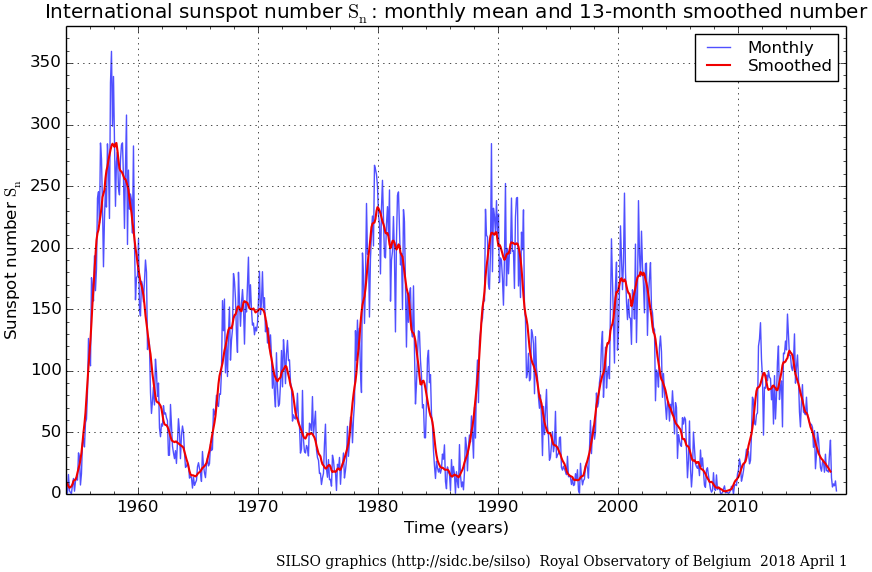
\includegraphics[width=0.6\textwidth]{figures_of_others/images/ROB_SSN_wolfmms.png}
	}{
		\caption[\lofimage{figures_of_others/images/ROB_SSN_wolfmms.png}Credit: \href{http://sidc.be/silso/monthlyssnplot}{SILSO data/image, Royal Observatory of Belgium, Brussels}, 2018.]
		{Monthly mean sunspot number (blue) and 13-month smoothed monthly sunspot number (red) since 1954. Credit: \href{http://sidc.be/silso/monthlyssnplot}{SILSO data/image, Royal Observatory of Belgium, Brussels}, 2018.}
		\label{fig:ROB_SSN_wolfmms}
	}
	\addtocontents{lof}{\smallskip\protect\center SILSO images can be freely downloaded as public data.\protect\footnote{SIDC/SILSO website, data policy at the bottom: \url{http://sidc.be/silso/home}}\medskip}
\end{figure}
%SIDC/SILSO permission request: permission not required
%image from:	http://sidc.be/silso/
There also exist long-term variations, such as secular cycles of different periodicity or the 70"~year Maunder~Minimum, during which from 1645 on almost no sunspots were observed, \citep{Maunder1890}.	%but: Zolotova2015: "The Maunder Minimum is Not as Grand as it Seemed to be"
The source of the variations in the solar cycle periods and amplitudes are variations in the meridional circulation, because their fluctuations are larger than those found in the differential rotation and in the convective motions \citep{Hathaway2015}.

%%% SSN prediction
As the SSN is commonly used as an indicator for solar activity, there exists interest in its prediction for the course of the actual and upcoming solar cycles. The continuing prediction of an already commenced activity cycle is reliable, but then the prediction of a cycle before it began is more difficult. Though, there are indications that the polar magnetic field strength during the preceding activity minimum is correlated to the strenght of the next solar cycle \citep{Schatten1987}. However, \citet{Hathaway2016} suggest that the predictability of solar cycles is generally limited -- accumulated uncertainty produced by stochastic motions in the convection zone makes predicitons further than the next solar cycle very unreliable.


\section{Heliospheric magnetic field}
\label{sec:heliospheric_magnetic_field}
%%% MBPs to canopy
In the quiet Sun during solar cycle minimum, open coronal regions -- coronal holes -- are the photospheric sources of the heliospheric magnetic field (HMF). Bright points between the granules on the photosphere are detected in G-band (\SI{430}{\nano\meter}) images. They are identified as magnetic flux tubes with field strenghts of \SIrange{100}{200}{\milli\tesla} \citep{Cranmer2005}. Together, these magnetic bright points (MBPs) cover around \SIrange{1}{2}{\%} of the solar surface and carry many times the flux that active regions do \citep{Sanchez_Almeida2010}. These thin flux tubes expand laterally in the low chromosphere and merge to homogeneous network fields, which expand and merge again to a large-scale canopy below the transition region (see \autoref{fig:Cranmer2005_fig1_ab}).
\begin{figure}[htb]
	\fcapside[\FBwidth]{
		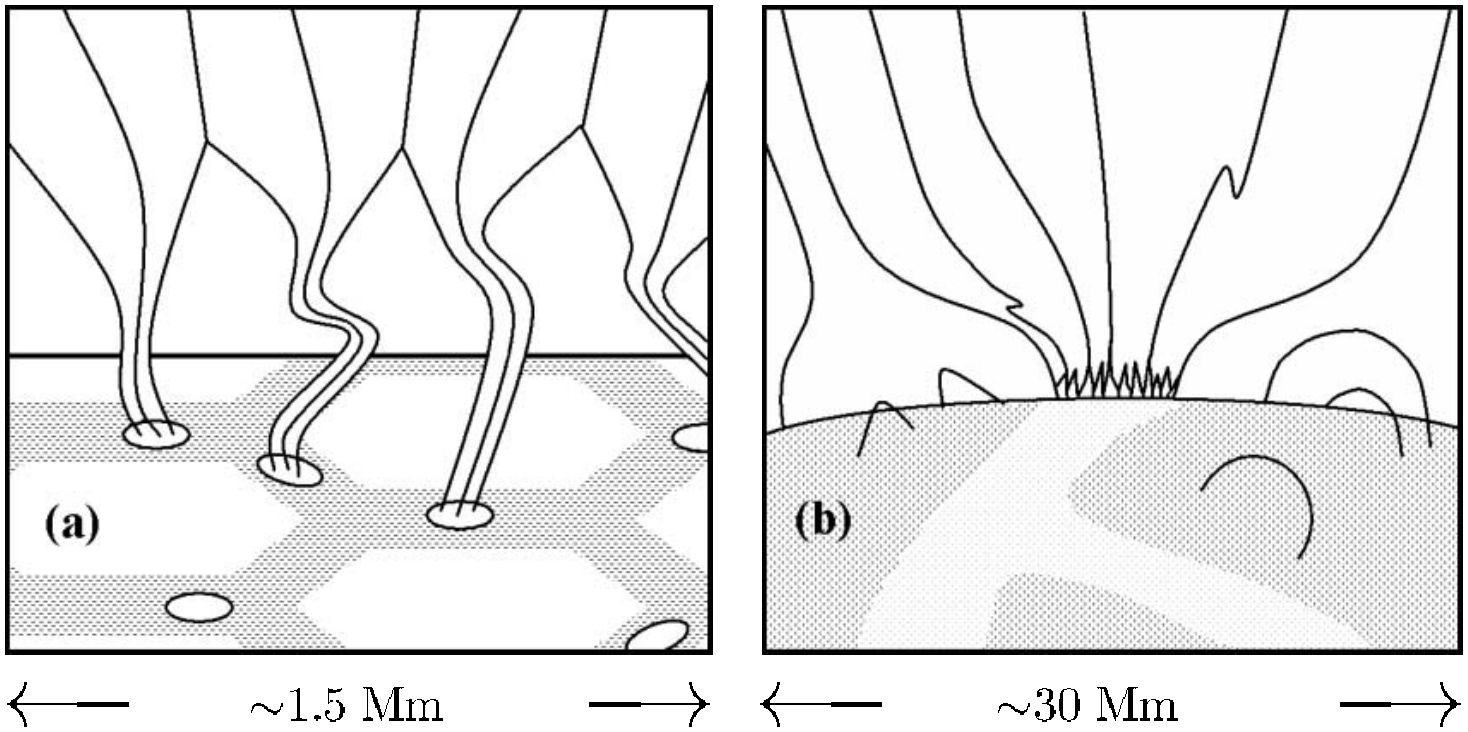
\includegraphics[width=0.6\textwidth]{figures_of_others/images/Cranmer2005_fig1_ab.png}
	}{
		\caption[\lofimage{figures_of_others/images/Cranmer2005_fig1_ab.png}Credit: {\citet[Fig.~1, panels (a) and (b)]{Cranmer2005}}, \textcopyright~AAS, reproduced with permission.]
		{Schemata of superradially expanding magnetic flux. (a) MBPs between granules on the photosphere are indicated by ellipses. The protruding lines are thin magnetic flux tubes that merge to a homogeneous network field. (b) Pictured is the network field which expands again to the large-scale canopy field of the lower corona. Credit: {\citet[Fig.~1, panels (a) and (b)]{Cranmer2005}}, \textcopyright~AAS, reproduced with permission.}
		\label{fig:Cranmer2005_fig1_ab}
	}
	\addtocontents{lof}{\smallskip\protect\center See the following email correspondence.\medskip
		\protect\lstinputlisting{figures_of_others/permissions/Cranmer2005_fig1_IOP_permission.txt}
		The related email attachment:
		\protect\lstinputlisting{figures_of_others/permissions/Cranmer2005_fig1_permission.txt}
	}
\end{figure}

%%% Alfvén waves
The MBPs' convective appearance and stochastic motions on the photosphere result in wavelike fluctuations that propagate upward through the superradially expanding flux tubes. There exist three types of magnetohydrodynamic (MHD) waves within the plasma: compressional fast- and slow-mode waves, and an incompressible wave mode, which is the result of bending magnetic field lines \citep{Alfven1942}, called shear Alfvén wave. Alfvén waves propagate with a characteristic speed along magnetic field lines. As they transport energy from the photosphere outwards, it is assumed that they play a major role in the coronal heating process and that the solar wind is accelerated up to the so-called Alfvén critical surface at around \SI{17}{\Rs}, where the local Alfvén speed equals the solar wind speed \citep{Sittler1999,Exarhos2000}. Alfvén waves are dominant in coronal regions that have open magnetic field lines and thus they leak into the fast solar wind \citep{Cranmer2005}. Within solar wind at \SI{1}{\au}, their average velocity is about \SI{57}{\km\per\s} \citep{Veselovsky2010} -- for more details about the Alfvén velocity see appendix \autoref{sec:alfvén_velocity}.

%%% field geometry from source surface on to heliopause
The coronal plasma in CHs expands superradially, following the magnetic field lines. However, the field strength decreases with increasing solar distance and at a distance of about \SI{2.5}{\Rs} the thermal pressure becomes larger than the magnetic pressure. Thereby the magnetic field gets frozen within the plasma and is carried by the solar wind radially outwards into the heliosphere. The distance from which the solar wind propagation gets released from the magnetic field lines is called the source surface \citep{Schatten1969} and the thermal to magnetic pressure ratio is called plasma beta -- for more details on plasma beta see appendix \autoref{sec:plasma_beta}. The magnetic field changes from superradial expansion below the source surface to a radial configuration above it, this field geometry is also visible in the total eclipse image in \autoref{fig:Tse2008_500_mo1}.

%%% heliospheric current sheet
Open field lines expand over adjacent closed field regions. Above the cusps of these regions' closed loops, the surrounding plasma flows encounter each other and stream outwards, forming so-called helmet streamers. Above the helmet streamers, magnetic boundaries are created by plasma flows, carrying opposite magnetic polarity. These boundaries constitute an extensive coronal neutral line around the Sun. Within the heliosphere, the two dominating magnetic polarity regions, originating from both solar magnetic poles, are separated by the extension of this neutral line: a large plasma boundary surface, called the heliospheric current sheet (HCS) \citep{Smith2001}.

Under solar cycle minimum conditions, the magnetic dipole axis is near the rotation axis and thus the HCS is roughly located near the equatorial plane, dividing both hemispheres. The analytical solar magnetic field model for solar minimum conditions, constructed by \citet{Banaszkiewicz1998}, shows this field geometry as seen in \autoref{fig:Banaszkiewicz1998_DQCS_model_raw}. The quadrupole part of their dipole plus quadrupole plus current sheet (DQCS) model considers the closed equatorial fields and allows equatorial outflow along the current sheet.
\begin{figure}[htb]
	\begin{floatrow}
		\ffigbox{
			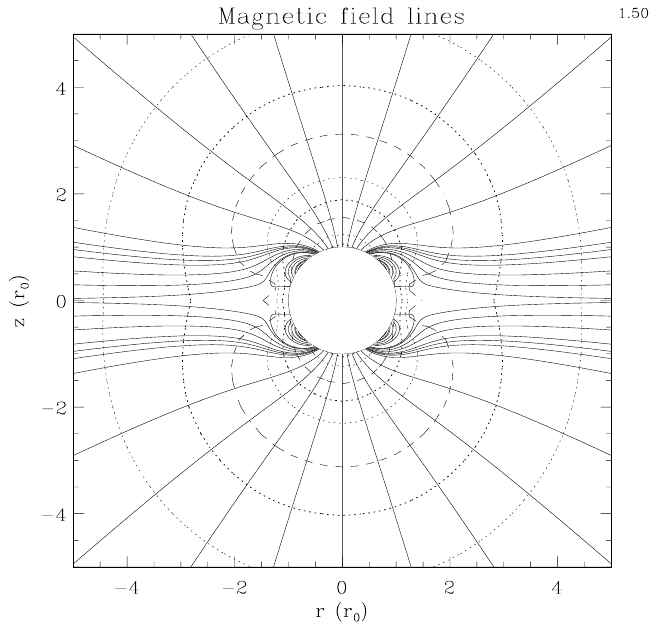
\includegraphics[width=0.45\Xhsize]{figures_of_others/images/Banaszkiewicz1998_DQCS_model_raw.png}
		}{
			\caption[\lofimage{figures_of_others/images/Banaszkiewicz1998_DQCS_model_raw.png}Credit: {\citet[Fig.~3]{Banaszkiewicz1998}}, \textcopyright~ESO, reproduced with permission.]
			{Model of the solar magnetic field geometry in the polar plane for solar cycle minimum. Magnetic field lines (solid) and constant field strength surfaces (dashed) from the DQCS model are plotted. The field line spacing does not represent the field strength but provides better detail where needed. Credit: {\citet[Fig.~3]{Banaszkiewicz1998}}, \textcopyright~ESO, reproduced with permission.}
			\label{fig:Banaszkiewicz1998_DQCS_model_raw}
		}
		\addtocontents{lof}{\smallskip\protect\center See the following document.\protect\\
			\protect\fbox{\protect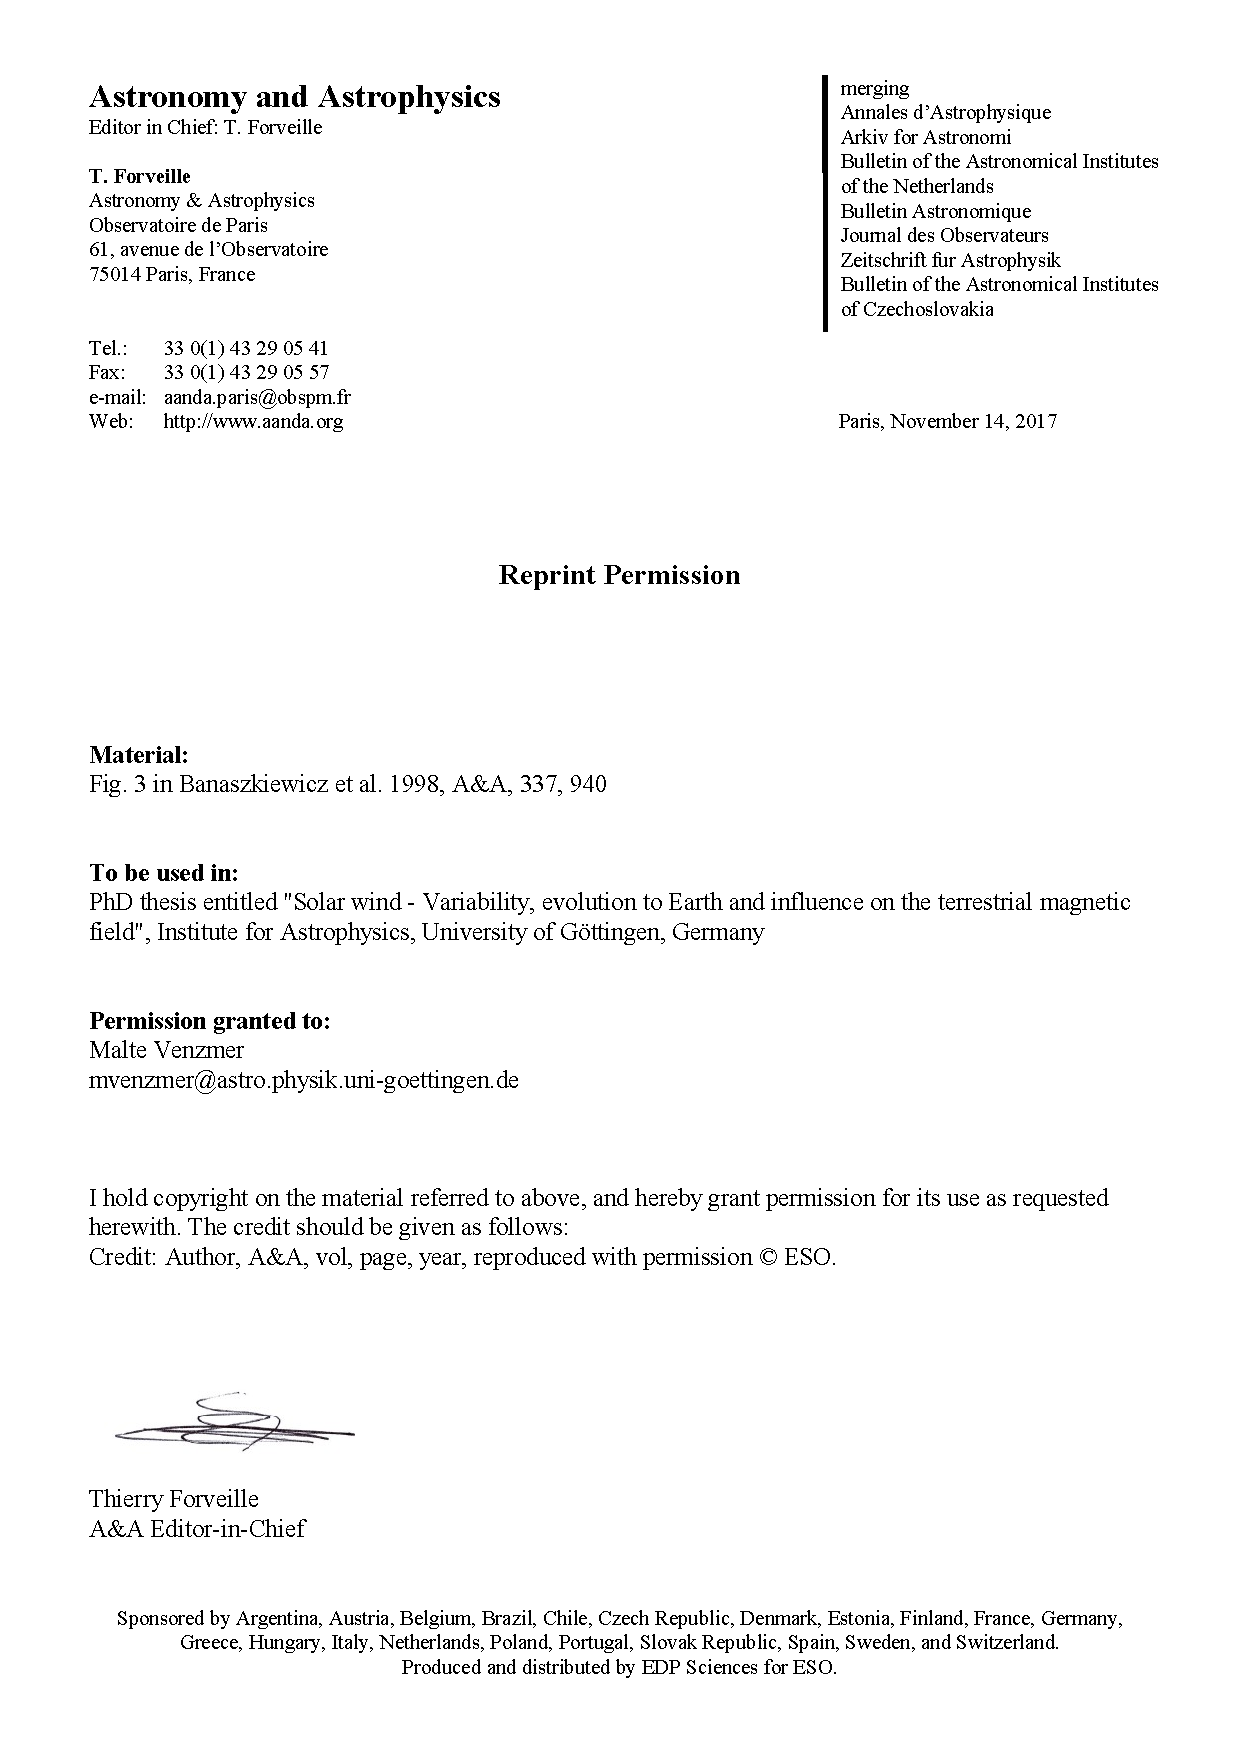
\includegraphics[width=0.6\textwidth,angle=90]{figures_of_others/permissions/permission_request_Banaszkiewicz1998_fig3.pdf}}
			\medskip
		}
		\ffigbox{
			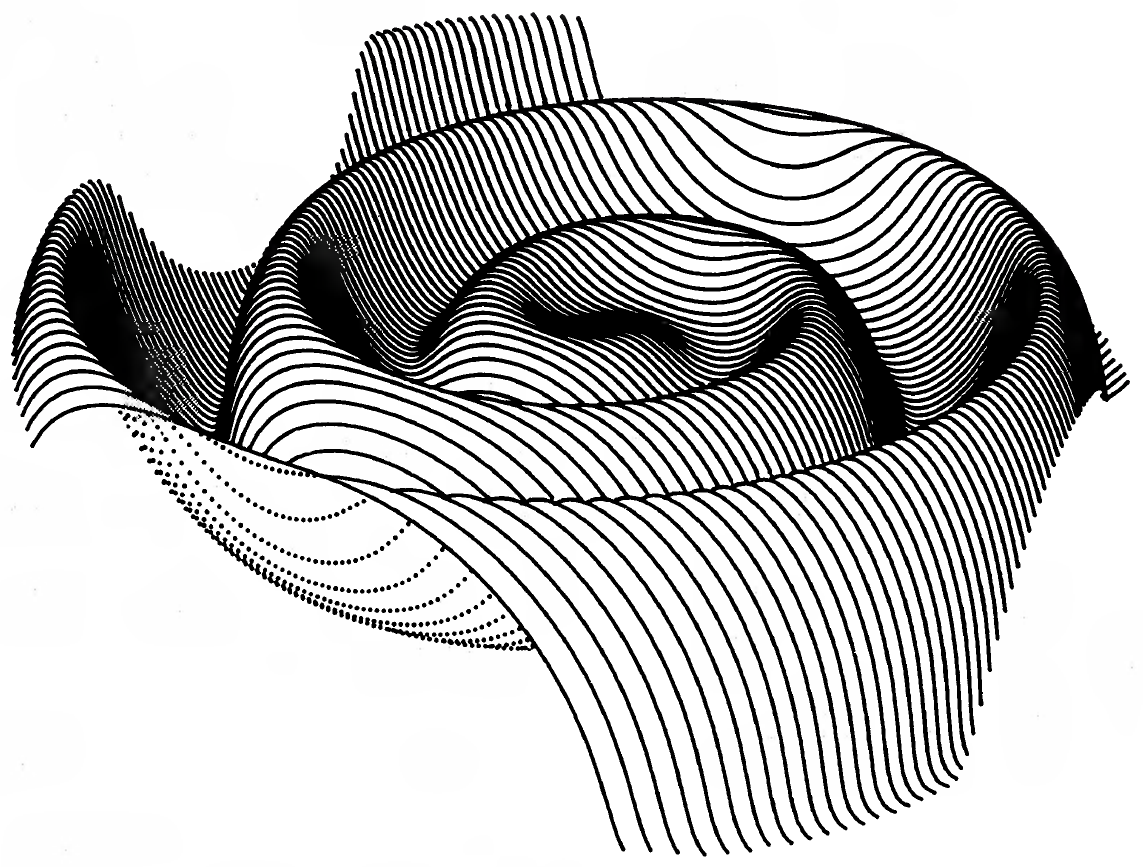
\includegraphics[width=\Xhsize]{figures_of_others/images/Jokipii1981_ballerina_HCS.png}
		}{
			\caption[\lofimage{figures_of_others/images/Jokipii1981_ballerina_HCS.png}Credit: {\citep[Fig.~2]{Jokipii1981}}, \textcopyright~AAS, reproduced with permission.]
			{A simple HCS model, where its wavy surface shape solely stems from a solar dipole tilt of \SI{15}{\degree} to the rotation axis. The figure's extend is \SI{25}{\au} across. Credit: {\citep[Fig.~2]{Jokipii1981}}, \textcopyright~AAS, reproduced with permission.}
			\label{fig:Jokipii1981_ballerina_HCS}
		}
		\addtocontents{lof}{\smallskip\protect\center See the following email correspondence.\medskip
			\protect\lstinputlisting{figures_of_others/permissions/Jokipii1981_permission.txt}
		}
	\end{floatrow}
\end{figure}
Commonly around solar minimum, the HCS's warped surface looks like a wavy ballerina skirt, due to the varying tilt angle between the dipole axis and the rotation axis, see \autoref{fig:Jokipii1981_ballerina_HCS}, and also due to local magnetic field variations \citep{Jokipii1981}.

During the field transition at solar maximum, the dipole axis rotates to lower latitudes, crosses the solar equator, and eventually the field ends up in a reversed dipole configuration \citep{Jones2003}. During this process, the HCS rotates almost rigidly together with the dipole axis and remains a single connected structure in the inner heliosphere \citep{Jones2003}. Hence during cycle maximum, the HCS has a very complex shape, is largely inclined to the solar equator, and reaches near-polar latitudes.

%%% Parker spiral
The solar wind source surface rotates with the Sun and thus shears the HMF into an Archimedean spiral pattern, adding an azimuthal component to the radial HMF. This geometry was anticipated by \citet{Parker1958} and is today called Parker spiral. The Parker spiral, viewed in the ecliptic plane, is illustrated in \autoref{fig:Owens2013_PFSS_Sectors_screenshot}. The solar rotation axis tilt of up to \SI{7.25}{\degree} to the ecliptic leads to a slight diving into both hemispheres of opposite polarity. Thus, together with the ballerina topology of the HCS, the Parker spiral has typically a structure of either two or four sectors of alternating magnetic polarity \citep{Ness1965}, which are separated by the HCS.
\begin{figure}[htb]
	\fcapside[\FBwidth]{
		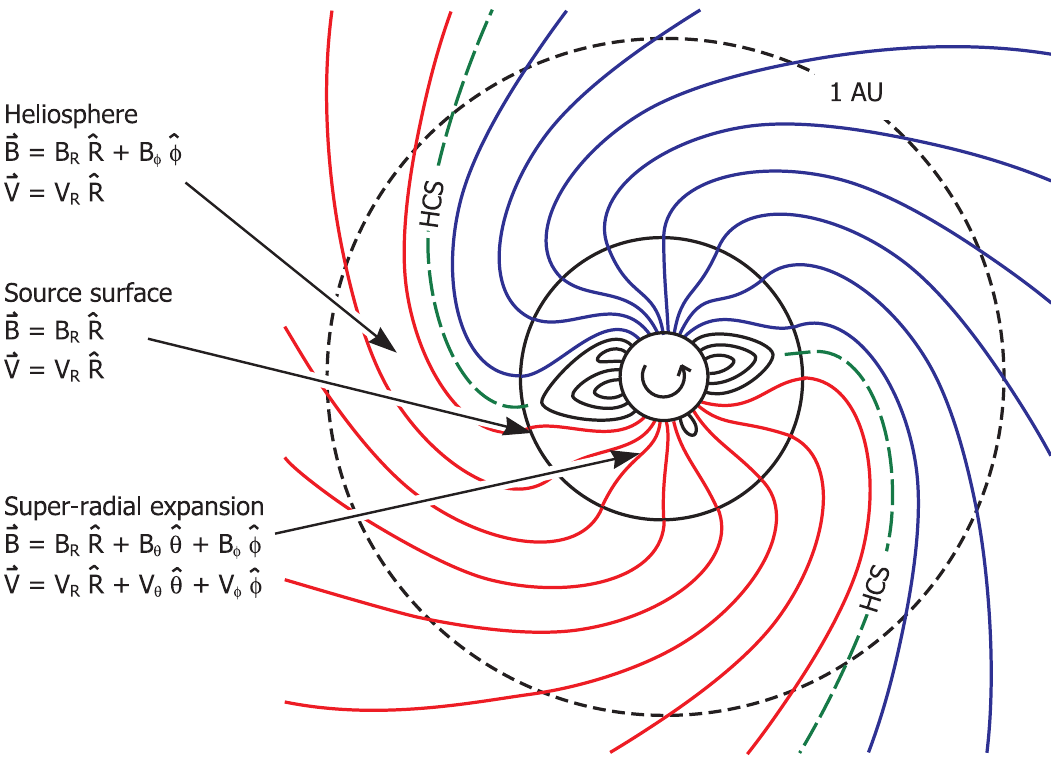
\includegraphics[width=0.6\textwidth]{figures_of_others/images/Owens2013_PFSS_Sectors_screenshot.png}
	}{
		\caption[\lofimage{figures_of_others/images/Owens2013_PFSS_Sectors_screenshot.png}Credit: {\citet[Fig.~1]{Owens2013}}, adapted from {\citet[Fig.~1]{Schatten1969}}, licensed under \href{https://creativecommons.org/licenses/by-nc/3.0/de/}{CC BY-NC 3.0 DE}.]
		{Illustration of the Parker spiral formation in the ecliptic plane outside the source surface. The HCS (green) is located between solar wind flows of opposite magnetic field polarity (red/blue). Credit: {\citet[Fig.~1]{Owens2013}}, adapted from {\citet[Fig.~1]{Schatten1969}}, licensed under \href{https://creativecommons.org/licenses/by-nc/3.0/de/}{CC BY-NC 3.0 DE}.}
		\label{fig:Owens2013_PFSS_Sectors_screenshot}
		%Owens2013 figure permission request: open access article
	}
	\addtocontents{lof}{\smallskip\protect\center See the permission to \autoref{fig:Owens2013_Heliosphere_screenshot}.\medskip}
\end{figure}

%other magnetic structures
The just described magnetic structures in the solar wind are overlaid by magnetic clouds (MCs) carried within CMEs. The MC's frequency and magnetic configuration vary with the solar activity cycle. Further, speed differences between solar wind streams, and between solar wind and CMEs cause enhanced field amplitudes and can result in shocks in the HMF.

%%% out to heliopause
That way, the HMF and its structures are carried out to the termination shock by the solar wind. MHD simulations, based on in-situ measurements of Voyager~1 and 2 within the heliosheath and based on IBEX observations of energetic neutral atoms, provide indications about the outer structure of the heliosheath. Behind the termination shock, the magnetic sector boundaries are compressed and they reconnect, forming magnetic bubbles \citep{Opher2011}. These bubbles -- unconnected to the HMF -- flow away to the heliosheath tail region. Even beyond the termination shock, the solar wind plasma seems confined and collimated by the twisted solar magnetic field and driven into a northern and a southern jet \citep{Opher2015}. Hence, the Sun's magnetosphere has likely a croissant-like shape with two turbulent tail-lobes, where eventually the solar wind and the HMF are being mixed into the interstellar medium.


\section{Solar wind}
\label{sec:solar_wind}
%%% sw history
It is observed that cometary tails lag a few degrees from the radial direction with respect to the Sun, sometimes they also show fluctuations and become kinked. As such behavior could not be explained by interaction with sunlight pressure, eventually \citet{Biermann1951} concluded that cometary ion tails are influenced by a continuous flow of particles from the Sun.	%Kivelson1995, p14+91
\citet{Parker1958} considered the consequences of Biermann's conclusions and built a solar wind model, adopting an expanding isothermal solar atmosphere. Parker also incorporated the implications for the solar magnetic field in his model and hence he laid the theoretical foundations for a continuous supersonic radial outflow of magnetized plasma. Thus, the existence of the solar wind was postulated before the first satellites measured it in~situ in 1959 \citep{Gringauz1960,Neugebauer1966}. Since that time, spacecraft are able to measure the solar wind almost continuously with magnetometer and plasma instruments in~situ (see \autoref{chap:data}). Pronounced solar wind structures, such as CMEs and streamers, become visible with the use of space-based coronagraph imagers. From Earth, the outflow of near-Sun solar wind can be observed during solar eclipses, see the eclipse photo in \autoref{fig:Tse2008_500_mo1}.

%%% plasma composition, parameter ranges and properties
The solar wind is a magnetized plasma consisting of electrons and ions. The ions are mainly composed of hydrogen, a small percentage of helium, and traces of oxygen, carbon, and other metals. The average abundance of helium is about \SI{4.5}{\%} and in slow wind at solar cycle minimum conditions less than \SI{2}{\%} \citep{Feldman1978,Schwenn1983,Kasper2012}.
The solar wind is commonly approximated by an ideal incompressible MHD plasma (viscosity $\mu = 0$ and electrical conductivity $\sigma = \infty$) and can be viewed as a neutral plasma. Also, its helium share is often viewed as being constant, in this case the proton density determines both the helium and electron densities. This work adopts these assumptions and treats the solar wind throughout as a proton plasma.

The properties of solar wind are highly variable in time and space. The key properties are determined by the values of the solar wind parameters magnetic field strength, proton velocity, density, and temperature. Their average magnitudes scale with solar activity, heliographic latitude, and solar distance. At a solar distance of Earth however, most of the time these parameter's typical values lie in the ranges \SIrange{3}{8}{\nano\tesla}, \SIrange{300}{500}{\km\per\s}, \SIrange{2}{8}{\per\cm\cubed}, and \SIrange{e4}{e5}{\K} (\citealp[p.~92]{Kivelson1995}; \citealt{Venzmer2018}). The low density of solar wind can be illustrated with a short comparison: 1~liter of air at standard pressure, expanded to a typical solar wind density of \SI{6.5}{\per\cm\cubed}, would occupy a volume of a cube with edge length of about \SI{155}{\km}.
% sw density considerations:\\
% 1 mol approx 24.7895 l/mol at 25 °C and 1 bar
% Avogadro constant N_A = 6.022140857(74)e23 mol−1
% 1 liter air @ 1 bar equates to 1/24.7895 mol = 2.4293e+22
% 2.4293e+22 / 6.5 cm-3 = 3.7374e+21 cm3 = 3.7374e6 km3 = (155 km)3
% 1 liter air @ 1 bar (need 24 ms for passing 1 dm2 area @ 15 km/h)\\
% equals\\
% 3.7e6 km3 = (155 km)3 solar wind @ 6.5 cm-3 (need 43900 a for passing 1 dm2 area @ 400 km/s)\\
Solar wind quantities, such as particle flux densities, mass flux, pressures, and plasma beta, can be derived from the four listed parameters. Having the parameters in the aforementioned ranges, the solar wind is a plasma with a beta mostly greater than unity, that is, the average solar wind carries the HMF and its motions are not influenced by the field direction (for more on plasma beta see appendix \autoref{sec:plasma_beta}).
% mean beta: 1.714\\	%from mean paper values
% low beta: 0.180\\	%from ranges above
% high beta: 8.444\\	%from ranges above

However, solar wind is structured by its different sources in the solar corona. It consists of fast continuous streams, slow variable flows, and transient CME events. These different flows have highly variable velocities, which result in compressed or rarefied regions at their interfaces. Additionally, the source region's magnetic field configuration organizes the HMF, transported within the solar wind plasma. Regardless, pronounced magnetic structures embedded in the solar wind, such as field polarity changes or magnetic clouds, still influence the properties of the plasma.

This multitude of structures is apparent in the two months -- beginning in May~2013 -- of in-situ measured solar wind, which I plotted as an example period in \autoref{fig:ACE_64s_v7_thesis_CIRs_2013-5-1_65_plot}.
\begin{figure}[htb]
	\centering
	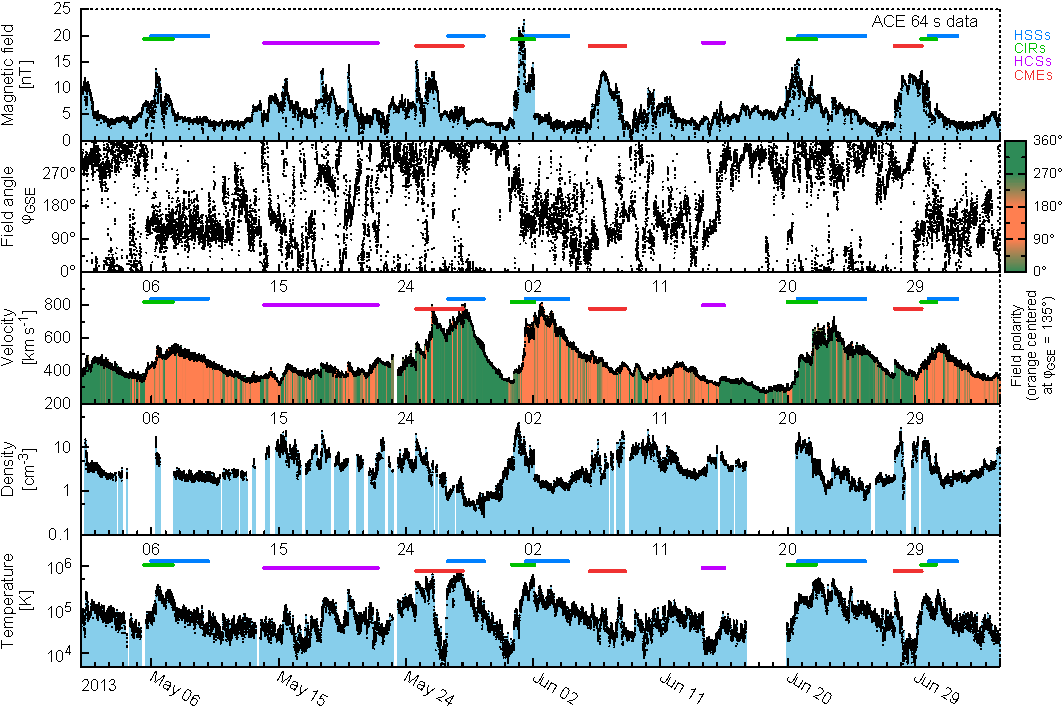
\includegraphics[width=\textwidth]{figures_of_mine/gnuplots/ACE_64s_v7_thesis_CIRs_2013-5-1_65_plot.pdf}
	\caption[\lofimage{figures_of_mine/gnuplots/ACE_64s_v7_thesis_CIRs_2013-5-1_65_plot.pdf}]
	{Solar wind with several structures, measured at L1 during the time period 1~May to 5~July in 2013. The parameters are the magnetic field strength, its field angle in the ecliptic in GSE~coordinates, the proton velocity, density, and temperature. I indicated periods of prominent solar wind structures with color bars: HSSs in blue, CIRs in green, HCSs in purple, and CMEs in red. In the velocity panel also the field polarity is color coded -- assuming a Parker spiral angle of \SI{135}{\degree} at L1. Blank periods indicate bad or missing data. The data are 64~s measurements from the ACE spacecraft.}
	\label{fig:ACE_64s_v7_thesis_CIRs_2013-5-1_65_plot}
	\addtocontents{lof}{\smallskip\protect\center I created the figure myself.\medskip}
\end{figure}
The IMF and solar wind ion parameters were measured with the MAG and SWEPAM instruments onboard the Advanced Composition Explorer (ACE) spacecraft, located around the first Lagrange point (L1). The data have a time resolution of 64~seconds and are obtained from the ACE~Science~Center web interface\footnote{ACE Science Center website: \urlfoot{http://www.srl.caltech.edu/ACE/ASC/}}.

Some general solar wind tendencies can be seen from this plot: The temperature of the solar wind scales with its stream velocity; compressed plasma regions enhance the magnetic field and the density; HCSs, magnetic sector boundaries, and MCs come with high densities and low temperatures; MCs in CMEs have high magnetic fields and low temperatures. I indicated the periods of occurring solar wind structures, that is, HSSs, CIRs, HCSs, and CMEs, with colored bars -- these types are further described in the following sections.

There exist a lot more aspects related to solar wind, i.e., MHD waves, the electron pitch angle, solar energetic particles, dust particles, and neutral energetic atoms. Yet, they are not covered here, because their relevance to the analyses in this work is considered minor.


\subsection{Slow and fast streams}
\label{sec:slow_and_fast_streams}
%%% fast and slow solar wind
It is observed at \SI{1}{\au} that the continuous solar wind comes in streams roughly focused at two major velocity ranges \citep{Neugebauer1966,Schwenn1983}, slow and fast streams with \SIrange{250}{450}{\km\per\s} and \SIrange{450}{800}{\km\per\s} respectively. Both types possess differences in their typical characteristics and ion compositions. Apart from its higher speeds, fast solar wind has most prominently lower proton densities ($\sim$\,\SI{3}{\per\cm\cubed}) and higher temperatures ($\sim$\,\SI{2e5}{\K}) than the slow solar wind, which has higher densities ($\sim$\,\SI{10}{\per\cm\cubed}) and lower temperatures ($\sim$\,\SI{4e4}{\K}) \citep{Schwenn1990}. The fast solar wind has a nature of coming in steady high-speed streams (HSSs) with a unique magnetic field polarity, whereas slow solar wind is much more variable in all its properties except its velocity \citep{Bame1977}. HSSs are further overlaid with Alfvén waves, which modulate the stream velocity with typical periods of \SIrange{15}{60}{\minute}.

%sources of fast wind
First soft X-ray observations of the corona, made during sounding rocket flights in the early 1970s, showed clearly that the fast solar wind emerges from extended areas of reduced X-ray emission, subsequently called coronal holes (CHs) \citep{Krieger1973,Hundhausen1977}. The magnetic field polarities found in CHs are associated with the magnetic field directions observed in HSSs, as seen in \autoref{fig:Hundhausen1977_fig10_cut}.
\begin{figure}[htb]
	\fcapside[\FBwidth]{
		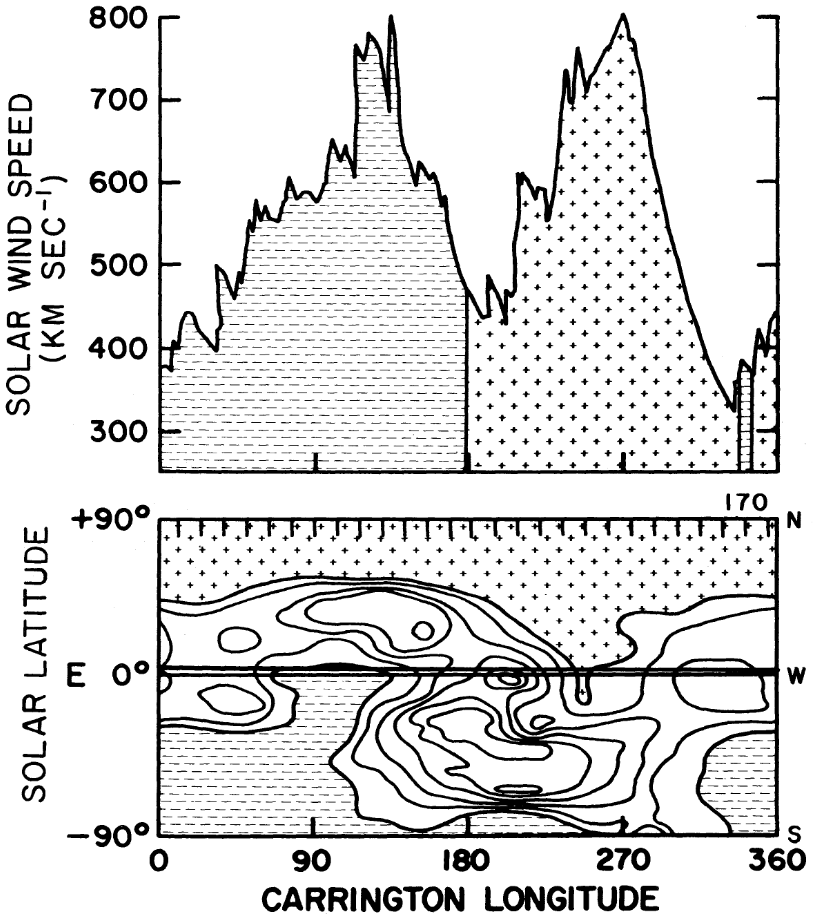
\includegraphics[width=0.5\textwidth]{figures_of_others/images/Hundhausen1977_fig10_cut.png}
	}{
		\caption[\lofimage{figures_of_others/images/Hundhausen1977_fig10_cut.png}]
		{Solar wind velocity with respect to its estimated source longitude (top) and coronal brightness contour map at \SI{0.5}{\Rs} above the photosphere (bottom) for the Carrington rotation 1616. The velocity is based on IMP spacecraft data, back-extrapolated to \SI{20}{\Rs}. Brightness values below a fixed threshold are shaded corresponding to the magnetic field polarity ($+$/$-$) of the underlying photosphere. The map is based on observations from the K-coronameter at the Manua~Loa Observatory. Credit: {\citet[Fig.~10]{Hundhausen1977}}, \textcopyright~Colorado Associated University Press, reproduced with permission.}
		\label{fig:Hundhausen1977_fig10_cut}
	}
	\addtocontents{lof}{\smallskip\protect\center additional permission for publishing pending...\medskip}
\end{figure}
In coronal regions with closed magnetic field lines, the plasma is trapped, though in CHs it can escape, following the open magnetic field lines outwards into space. Wave-particle interactions heat and accelerate the ions in CHs, leading to the emission of a fast solar wind \citep{Hollweg2002}. Superradial expansion of the magnetic field lines in the corona has an influence on the wind speed -- actually the expansion factor is anticorrelated with the final wind velocity \citep{Wang1990}. As the field expansion is larger near the border of CHs, faster wind emerges from the mid regions of CHs, forming into HSSs. However, there are indications that the slow and fast solar wind are not only generated at different sources but from distinct mechanisms \citep{McGregor2011b}.

%sources of slow solar wind
The high variability in the slow solar wind points to the existence of different types of slow wind flows, originating from separate coronal locations and mechanisms \citep{Schwenn1983}. It is still under debate if the variability is produced by the formation mechanism of the slow solar wind or if the variability is caused during the acceleration/propagation phase \citep{Sanchez-Diaz2016}. Still, at least a part of its variability can be attributed to the interactions between slow and fast solar wind, which result in a general reduction in velocity differences and thus let solar winds of different speeds (having different properties as well) converge to a common intermediate speed regime in the range \SIrange{400}{500}{\km\per\s} \citep{McGregor2011a,Sanchez-Diaz2016}. Studies using remote white-light tracing of coronal material and in-situ measurements of solar wind suggest that multiple sources of slow solar wind flows exist \citep{Wang2000,Kilpua2016}. To the best of my knowledge, the generally considered sources are listed in the following:
\begin{itemize*}
	\item CH boundaries and small CHs, because their plasma outflow is slower due to the high superradial expansion of its open field lines \citep{Wang1990}.
	\item CH boundaries, when trapped plasma is released by reconnection between open and closed field lines \citep{Madjarska2004}.
	\item Helmet/pseudo-streamers in active regions, where transient plasma blobs are released from the cusps of closed field loops \citep{Wang1998,Wang2000}. This slow and dense material is associated with the heliospheric plasma sheet belt.
	\item Edges of active regions, which have hot plasma outflows with a single mangetic polarity \citep{Kojima1999}.
	\item Jets originating from coronal bright points might contribute to the slow solar wind \citep{Subramanian2010}.
	\item Slow unidentified CMEs can be a source of slow wind as well.
\end{itemize*}
% Kilpua2016 generally suggested sources:\\
% - CH boundaries, the plasma is slow due to superradial expansion of open field lines\\
% - transient plasma blobs that are released from the helmet/pseudo-streamers\\
% - plasma released by reconnection between open and closed field lines at the coronal hole boundaries\\
% - hot outflows with speeds up to ∼100~km/s from the edges of active regions, first reported by Kojima1999\\
% - jets originating from coronal bright points\\

It is found to be difficult to use in-situ measurements for tracing the slow solar wind flow types to different origins and distinguishing between them, because most properties are also highly variable in time \citep{Kilpua2016}. However, some indicators show tendencies to differentiate between the slow winds from different source regions. Some notable indicators are: elemental ion ratios, heavy ion charge states, and the specific entropy.

The elemental composition of the coronal plasma varies with height/location in the solar atmosphere, therefore the solar wind's elemental ion ratios (e.g., $\text{He}/\text{H}$, $\text{Fe}/\text{O}$) are used to determine its origin.
The charge states of coronal heavy ions depend on the local temperature. However, the density of the outwards expanding plasma decreases fast, preventing further ionization/recombination. The charge states decouple from the local temperature and freeze~in still close to the Sun. Thus, heavy ion charge ratios (e.g., $\text{C}^{+6}\!/\text{C}^{+4}$, $\text{O}^{+7}\!/\text{O}^{+6}$) in the solar wind track the coronal source temperature and especially the $\text{C}^{+6}\!/\text{C}^{+4}$ ratio is sensitive to the solar wind type \citep{Landi2012}.
At solar minimum the specific proton entropy is found to correlate with the $\text{O}^{+7}\!/\text{O}^{+6}$ ratio and thus able to trace slow solar wind sources as well \citep{Pagel2004}.
%specific entropy: $\ln\left(T_\text{p}/n_\text{p}^{\gamma - 1}\right)$ ($\gamma = 1.5$)

%solar activity dependence
The solar wind stream pattern varies strongly with solar activity. The Sun's ordered dipole structure during solar cycle minima leads to polar regions with open magnetic fields, constituting large coronal holes, and to a large equatorial belt region with closed magnetic fields -- this state is clearly visible in Figures~\ref{fig:Tse2008_500_mo1} and \ref{fig:Banaszkiewicz1998_DQCS_model_raw}. This state results in fast solar wind coming exclusively from the poles and higher latitudes, whereas active regions form an equatorial streamer belt around the Sun, emitting slow solar wind. This structure was confirmed from solar wind speed measurements done by the Ulysses spacecraft, which flew in an out-of-ecliptic solar orbit and whose mission covered a duration of more than one solar cycle \citep{McComas200809}, see \autoref{fig:McComas2008_Ulysses_orbit}.
\begin{figure}[htb]
	\centering
	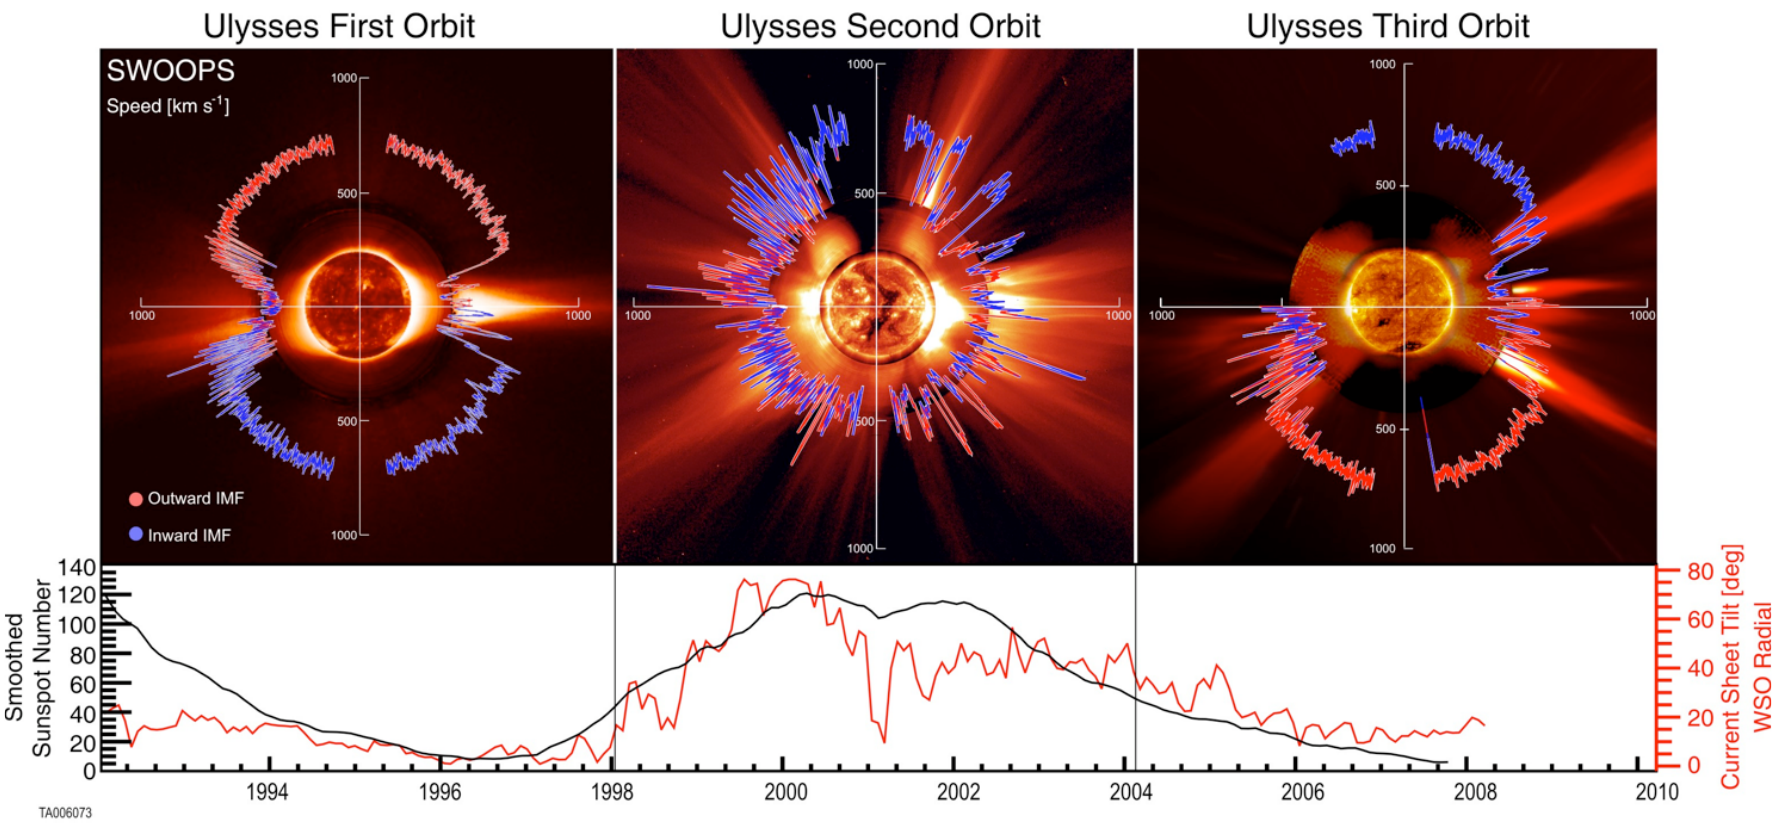
\includegraphics[width=\textwidth]{figures_of_others/images/McComas2008_Ulysses_orbit_.png}
	\caption[\lofimage{figures_of_others/images/McComas2008_Ulysses_orbit_.png}Credit: {\citet[Fig.~1]{McComas200809}}, \textcopyright~American Geophysical Union, reproduced with permission.]
	{Solar wind velocity and magnetic field polarity (red/blue) with respect to heliographic latitude for the three orbits of the Ulysses spacecraft during low and high solar activity (upper panels). The data starts top left and runs couterclockwise. The corresponding smoothed SSN (black) and HCS tilt angle (red) are plotted beneath. The background consists of solar images for solar cycle~22 minimum (1996-08-17), solar cycle~23 maximum (2000-07-12), and solar cycle~23 minimum (2006-03-28). The solar disk, inner corona, and outer corona images are from SOHO/EIT (Fe~XII at \SI{1950}{\nano\meter}), Mauna~Loa K~coronameter (\SIrange{700}{950}{\nano\meter}), and SOHO/C2 white light coronagraph. Credit: {\citet[Fig.~1]{McComas200809}}, \textcopyright~American Geophysical Union, reproduced with permission.}
	\label{fig:McComas2008_Ulysses_orbit}
	\addtocontents{lof}{\smallskip\protect\center See the document on the next page.
		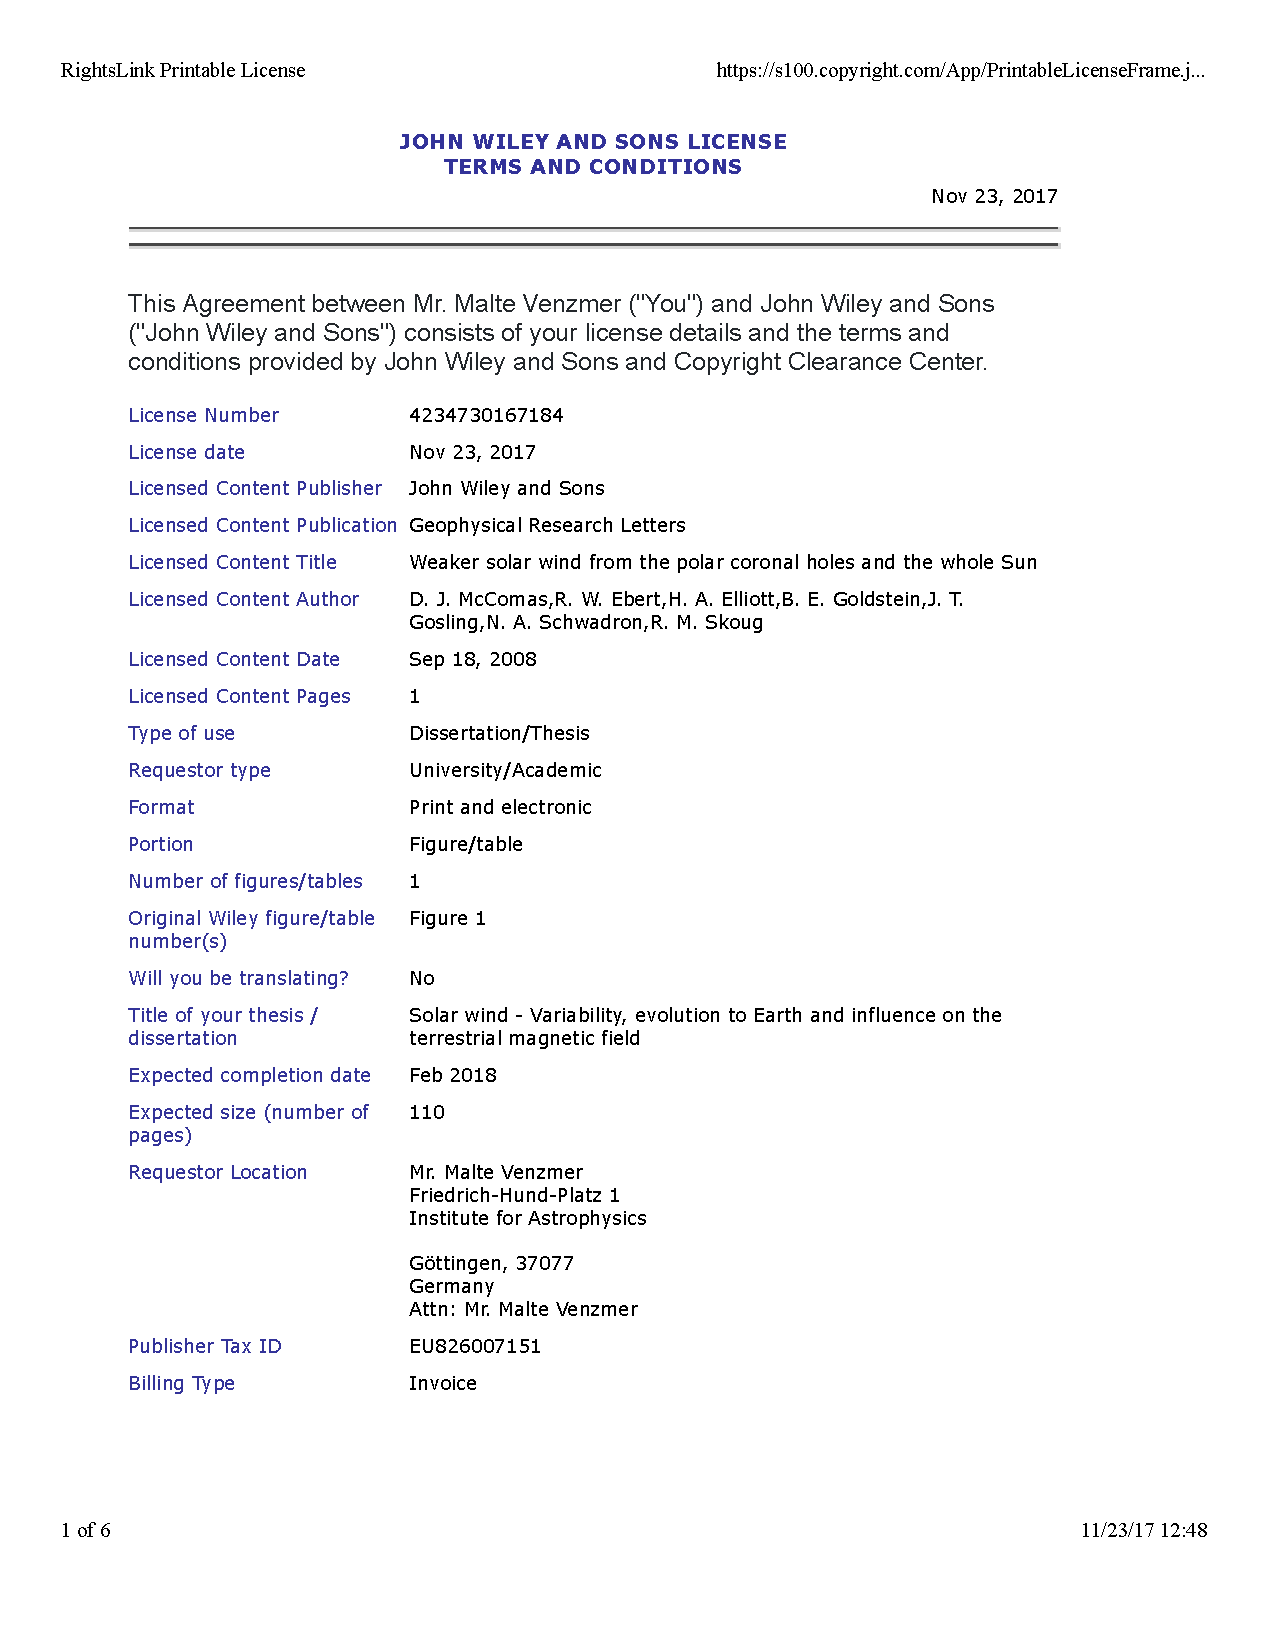
\includepdf[pages={-},nup=2x3,delta=1cm 2mm,column=true,frame=true,noautoscale=true,scale=0.32]{figures_of_others/permissions/permission_request_McComas2008a_fig1.pdf}
	}
\end{figure}
%figure source: http://onlinelibrary.wiley.com/doi/10.1029/2003GL017136/full
%McComas200809: (a–c) Polar plots of the solar wind speed, colored by IMF polarity for Ulysses' three polar orbits colored to indicate measured magnetic polarity. In each, the earliest times are on the left (nine o'clock position) and progress around counterclockwise. (d) Contemporaneous values for the smoothed sunspot number (black) and heliospheric current sheet tilt (red), lined up to match Figures 1a–1c. In Figures 1a–1c, the solar wind speed is plotted over characteristic solar images for solar minimum for cycle 22 (8/17/96), solar maximum for cycle 23 (12/07/00), and solar minimum for cycle 23 (03/28/06). From the center out, we blend images from the Solar and Heliospheric Observatory (SOHO) Extreme ultraviolet Imaging Telescope (Fe XII at 1950 nm), the Mauna Loa K coronameter (700–950 nm), and the SOHO C2 white light coronagraph.
The transition of the solar magnetic field during the solar cycle maxima induces the chaotic appearance of closed magnetic fields at higher latitudes and even at the poles. Further, coronal holes begin to invade parts of the equatorial region, this leads to recurring phases of HSSs in the ecliptic. This can be seen from the solar wind period in \autoref{fig:ACE_64s_v7_thesis_CIRs_2013-5-1_65_plot}, where recurrent HSSs of the same field polarity but changing peak velocity exist -- beginning on 6~May, 2~June, and 29~June 2013. The succeeding streams of different velocity result in interaction regions and alternating magnetic polarities result in magnetic sector boundaries.


\subsection{Stream interaction regions}
The sources of the slow and fast solar wind rotate together with the Sun. Their uneven distribution on the solar surface -- due to a significant inclination of the dipole axis or variations of the solar magnetic field -- lead to the alternation of slow and fast wind streams that flow into the heliosphere \citep{Owens2013}.
% stream interfaces
In case of a fast stream being followed by a slow stream, a rarefaction region expands at their interface. If it is the other way around, the stream of fast solar wind catches up to that of slow wind ahead of it and a compression region forms at their interface, which is encompassed by two compressional waves \citep{Balogh2009}. The latter are stream interaction regions (SIRs) and they take the shape of spiral fronts, as seen in the left panel of \autoref{fig:Owens2013_CIR_2panel_screenshot}.
\begin{figure}[htb]
	\fcapside[\FBwidth]{
		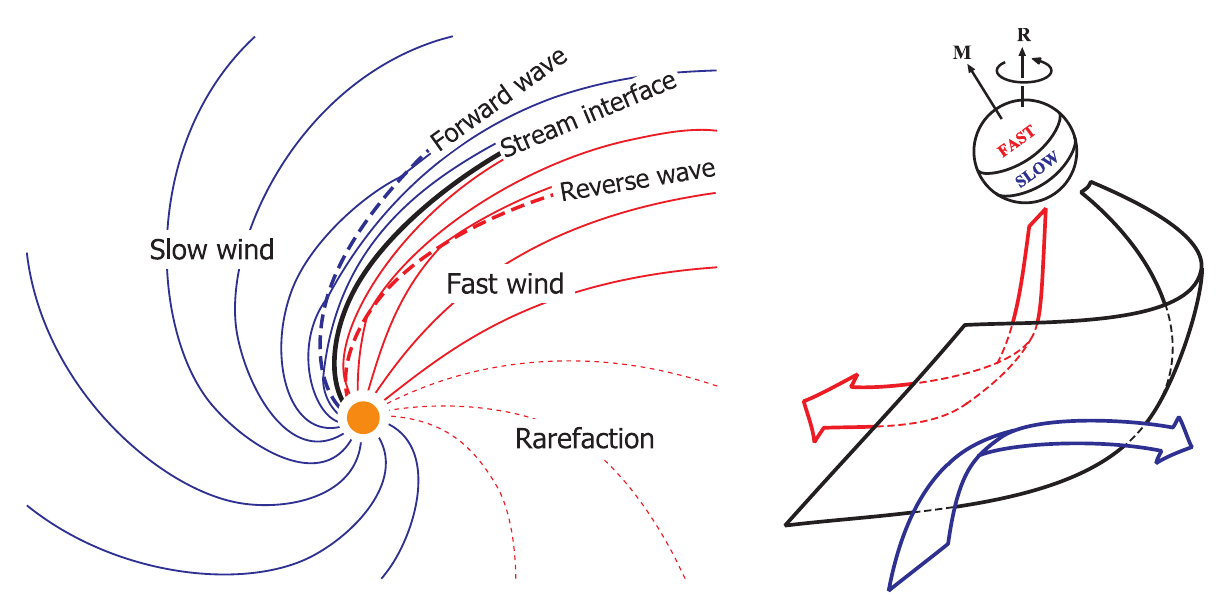
\includegraphics[width=0.6\textwidth]{figures_of_others/images/Owens2013_CIR_2panel_screenshot.png}
	}{
		\caption[\lofimage{figures_of_others/images/Owens2013_CIR_2panel_screenshot.png}Credit: {\citet[Fig.~7]{Owens2013}}; right panel adapted from {\citet[Fig.~2]{Pizzo1991}}, licensed under \href{https://creativecommons.org/licenses/by-nc/3.0/de/}{CC BY-NC 3.0 DE}.]
		{Schemata of the formation of a stream interface (left) and the deflection of streams along the interface (right). The stream interface (black) is located between regions of slow (blue) and fast (red) solar wind. Credit: {\citet[Fig.~7]{Owens2013}}, right panel adapted from {\citet[Fig.~2]{Pizzo1991}}, licensed under \href{https://creativecommons.org/licenses/by-nc/3.0/de/}{CC BY-NC 3.0 DE}.}
		\label{fig:Owens2013_CIR_2panel_screenshot}
	}
\end{figure}
%Owens2013 figure permission request: open access article
%A sketch of a stream interaction region. Left: Looking down on the ecliptic plane. Magnetic field lines within fast (slow) wind, shown in red (blue), become aligned with the stream interface by the reverse (forward) wave. Right: a view from Earth. The magnetic axis, M, and therefore the wind speed belts, are inclined to the rotation axis, R. The point in the heliosphere at which fast wind is able to catch up to the slow wind ahead of it is the stream interface (SI), which forms a spiral front in the heliosphere, shown as the black-outlined curved surface. In the frame of reference of the SI, both fast and slow wind flow toward the SI. Fast (slow) wind, shown by the red (blue) arrow, is slowed (accelerated) and deflected along the SI in the direction counter to (along) solar rotation. Right panel adapted from Pizzo (1991).

% CIRs
When the solar dipole field is in a quasi-stable configuration, SIRs can stay for multiple solar rotations, recurrently sweeping over the heliosphere in 27-day periods \citep{Gosling1972}. Hence, they are referred to as co-rotating interaction regions (CIRs) \citep{Smith1976,Balogh1999}.
% time
In the ecliptic at \SI{1}{\au}, CIRs occur commonly during the declining phase of the solar cycle when polar CHs form equatorial extensions \citep{Balogh2009}.

% deflections
The spiral shape of the stream interfaces and their inclination to the solar rotation axis lead to a deflection of both streams \citep{Balogh2009}. Due to the fast and slow streams' collision, the fast wind is decelerated and the slow wind is accelerated and their flow directions are systematically deflected away from the interface, as shown in the right panel of \autoref{fig:Owens2013_CIR_2panel_screenshot}.

% shocks
The plasma pressure inside SIRs is increasing with heliocentric distance and therefore, the leading and trailing compressional waves form into foreward and reverse shocks -- typically at solar distances between \SIrange{2}{10}{\au} \citep{Smith1976,Balogh2009}. The solar wind speed increases abruptly at both shock fronts.
% MIRs
With increasing solar distance, the leading and trailing shock fronts travel away from the stream interface. This widens the interaction regions and eventually they gain on the close-by interaction regions \citep{Burlaga1984}. Beyond \SI{10}{\au} they fuse to merged interaction regions, which are narrower and more compressed \citep{Burlaga1985}.

% in-situ signatures of SIRs
Due to the compression within SIRs, the magnetic field strength and the plasma density are higher than in the ambient streams. These signatures can be seen in the in-situ solar wind plot in \autoref{fig:ACE_64s_v7_thesis_CIRs_2013-5-1_65_plot}. The CIRs on 5~May, 1~June, and 29~June 2013 are followed by recurrent HSSs and they contain sector boundaries as well. They are not yet accompanied by strong shocks owing to the measurement location at \SI{1}{\au}.


\subsection{Heliospheric current sheet}
The heliospheric current sheet (HCS), the boundary surface between solar wind streams of opposite magnetic polarity, is formed by open magnetic fluxes, expanding from both sides over closed field regions and coming into contact above. At the boundary between open and closed fields, local coronal plasma gets released and flows slowly between the fast wind streams along the current sheet into the heliosphere, creating a helmet streamer. This is why near the Sun, the HCS is typically located within slow solar wind stemming from the coronal streamer belt \citep{Owens2013}. However, with increasing solar distance, the shock wave of an adjacent SIR can pass the HCS, so that sector boundaries are often found to be embedded within SIRs \citep{Gosling1999}.

% heliospheric plasma sheet
When sector boundaries in the solar wind are observed in~situ, they come with significant depletions in $\text{He}^{++}\!/\text{H}^+$ values \citep{Borrini1981}. The other solar wind parameters, such as velocity, density, and temperature, change with distance from the HCS as well \citep{Smith2001}. The HCS region itself is quite narrow with a thickness of around \SIrange{3000}{10000}{\km}; it is embedded in a region of 20--30~times its thickness, the heliospheric plasma sheet (HPS) \citep{Winterhalter1994}. The HPS contains the magnetic polarity reversal and is of low magnetic field strength and high density, resulting in a significantly enhanced value of plasma beta \citep{Crooker2004}. In the slow solar wind, the HPS can also be identified from its particularly low specific entropy, arising from its low temperature and high density \citep{Kilpua2016}.


\subsection{Coronal mass ejections}
\label{sec:coronal_mass_ejections}
Coronal mass ejections (CMEs) are eruptions of coronal magnetized plasma, which expand within hours to bubbles with sizes of a few solar radii. They continuously expand further while moving farther away from the Sun into the heliosphere with velocities often surpassing even the high speed solar wind. When measured in-situ in interplanetary space, they are often called interplanetary CMEs (ICMEs). They are transient structures found to be embedded in the ambient slow and fast solar wind streams, having durations of a few days. CMEs make up about \SI{5}{\percent} of the solar wind's flow share during solar cycle minima, but can represent up to about \SI{50}{\percent} during solar cycle maxima \citep{Richardson2012}. Indeed, their frequency correlates with the sunspot number \citep{Hildner1976} and follows solar activity in amplitude and phase \citep{Webb1991}.

Long before the origins of geomagnetic disturbances were actually attributed to CMEs, a solar influence was identified as their source by \citet{Carrington1859}. Indeed, CMEs are the major drivers for strong geomagnetic storms, because they carry the most extreme conditions found in the solar wind. Thus, they are of major importance to space weather -- their impacts on the terrestrial magnetosphere are covered in \autoref{sec:space_weather}.

% CME formation, flares
I will cover the CME formation processes only briefly, because this work is focused on in-situ measurements. Generally speaking, CMEs are products of the instability in the coronal magnetic field. The solar differential rotation wraps the coronal magnetic field, which is rooted at the surface. Accumulated tension and emerging magnetic flux eventually initiate sudden field reconfigurations. These field line reconnections result in a lower state of potential energy, releasing a lot of energy in form of solar X"~ray flares and CMEs. Indeed, CMEs are often associated with flares and eruptive prominences, coming from their source regions \citep{Webb1987}. The sources of CMEs are located near active regions and are frequently identified with eruptive prominences \citep{Subramanian2001}.

% flux ropes, filaments, prominences
CMEs emerge from coronal magnetic flux rope structures that hold plasma filaments embedded along their base \citep{Webb1987,Cremades2004}. Reconfiguration of the ambient magnetic field can lead to a release and a subsequent ascend of the flux rope through the corona. During this process, the filament is lifted by the flux rope and forms a prominence eruption. The accompanying sudden magnetic reconnections often cause a multitude of other dynamic coronal phenomena: enhanced X"~ray flaring; the formation of post-eruptive arcades where the filament disappeared; local decreases in soft X"~ray intensity (coronal dimmings) due to depletion of the plasma density caused by magnetic field expansion; and large-scale coronal disturbances observed in extreme ultraviolet (EUV"~waves) that can spread across the whole corona.

% SEPs and radio bursts
The onset of CMEs is often accompanied by solar energetic particles (SEPs) and by solar radio bursts. SEPs consist of protons, electrons, and ions with relativistic energies that can cover the distance to Earth within half an hour and pose a radiative threat to humans in space. The intensity of energetic protons correlates well with the CME speed \citep{Kahler1978} and it is established that these coronal particles are accelerated by shocks formed in front of the rapidly expanding magnetic structures of CMEs in the corona \citep{Cliver1982,Gosling1993}. Solar radio bursts are radio emissions from the corona that change over time in frequency space. There are different kind of radio bursts, but especially type~II radio bursts are seen as indicators for coronal shocks that accelerate electrons. 
They are emitted in the low corona and are drifting to lower frequencies over time. There is still a debate whether type~II bursts originate from flares or CMEs, favoring the latter \citep{Gosling1993,Cliver2005,Cho2011}.
% % radio bursts
% % https://www.nrao.edu/astrores/gbsrbs/Pubs/AJP_07.pdf
% % http://www.astron.nl/lofarscience2015/Documents/LSW/June_2/Session_3/reid.pdf
% A solar radio burst is a structure in frequency space that changes with time.\\
% type~II radio burst (drift to low frequencies): fundamental and second–harmonic bands; evidence for shocks in the corona, rendered visible by the radiation of electrons that they accelerate. There is almost always a delay between the flare onset and the start of Type II emission. the shocks that produce Type II bursts are maybe always being driven by CMEs\\
% type~III radio burst (spikes): parallel to flares; track electron beams through decreasing sw plasma density along Parker spiral; frequency scales with distance\\
% type~IV radio burst: broadband quasi–continuum features associated with the decay phase of solar flares. They are attributed to electrons trapped in closed field lines in the post–flare arcades\\

CMEs were detected in the white-light observations of the K"~corona made by the first space-based coronagraphs on board the OSO~7 satellite \citep{Tousey1973} and the Skylab space station \citep{MacQueen1974}. These observations show the steady outflow of solar wind, broken by intermittent ejections of coronal plasma. Subsequently, the kinematic properties of CMEs were identified from the white-light images \citep{MacQueen1980}. Now, coronagraphs observe the corona and hence CMEs continuously from the first Lagrange point (L1) in front of Earth with the SOHO spacecraft and from changing equatorial perspectives with the STEREO~Ahead (A) and Behind (B) spacecraft. The image of the corona from 23~September 2012, made by the SECCHI/COR2 coronagraph onboard STEREO~A, shows a CME to the top right, see \autoref{fig:CME_COR2_0120923_182400_dbc2A}.
\begin{figure}[htb]
	\begin{floatrow}
		\ffigbox{
			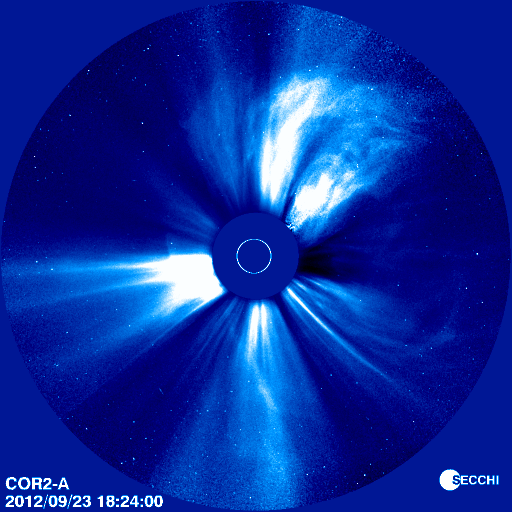
\includegraphics[width=0.45\textwidth]{figures_of_others/images/CME_COR2_0120923_182400_dbc2A.png}
		}{
			\caption[\lofimage{figures_of_others/images/CME_COR2_0120923_182400_dbc2A.png}Courtesy of \href{https://stereo.gsfc.nasa.gov/gallery/copyright.shtml}{STEREO/COR2 consortium (NASA)}.]
			{Image of the solar corona out to \SI{15}{\Rs} from 23~September 2012 taken by the SECCHI/COR2 coronagraph onboard the STEREO~A spacecraft. The solar disk is covered by the occulter disk and its position is indicated by the white circle. The bright blob to the top right is the CME; the smooth elongated radial lines are solar wind streamers. Courtesy of \href{https://stereo.gsfc.nasa.gov/gallery/copyright.shtml}{STEREO/COR2 consortium (NASA)}.}
			\label{fig:CME_COR2_0120923_182400_dbc2A}
		}
% https://stereo.gsfc.nasa.gov/gallery/copyright.shtml
		\ffigbox{
			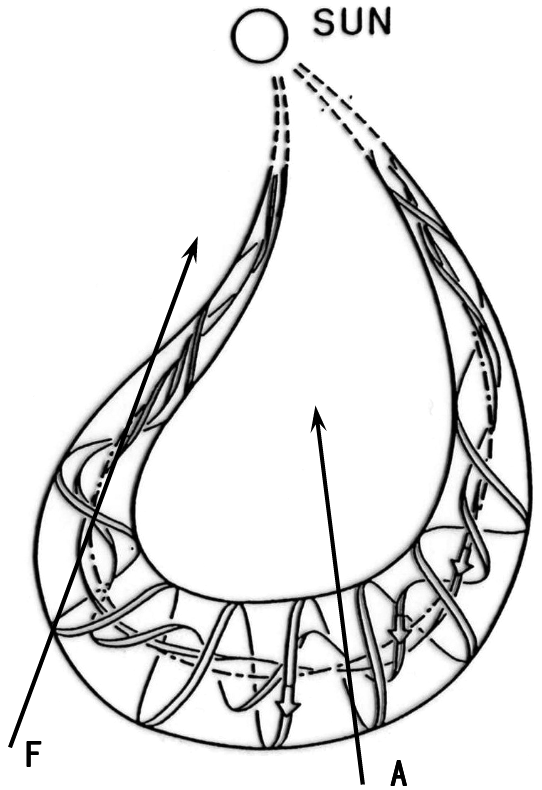
\includegraphics[width=0.3\textwidth]{figures_of_others/images/Marubashi2007_fig1.png}
		}{
			\caption[\lofimage{figures_of_others/images/Marubashi2007_fig1.png}Credit: {\citet[Fig.~1, panel (a)]{Marubashi2007}}, licensed under \href{https://creativecommons.org/licenses/by/3.0/}{CC BY 3.0}.]
			{Schema of a magnetic flux rope structure in a CME. The arrows depict passings through its flank (F) and its apex (A). Credit: {\citet[Fig.~1, panel (a)]{Marubashi2007}}, licensed under \href{https://creativecommons.org/licenses/by/3.0/}{CC BY 3.0}.}
			\label{fig:Marubashi2007_fig1}
		}
	\end{floatrow}
\end{figure}

It was early determined by \citet{Gold1962} that solar ejecta should drive shock waves ahead. In fact, shocks with trailing low proton temperatures caused by fast CMEs were then found in in-situ measurements \citep{Gosling1973,Gosling1974}. \citet{Burlaga1981} analyzed magnetic field and plasma in-situ data from five spacecraft and identified a shock wave with a trailing turbulent sheath region followed by an organized helical magnetic structure that they called a magnetic cloud (MC). MCs have an enhanced magnetic field, a smooth rotation in the azimuthal magnetic field component and they show low densities and temperatures \citep{Burlaga1981}. Thus, MCs have a low thermal to magnetic pressure ratio (i.e., a small plasma beta) and the magnetic field dominates the plasma. Furthermore, the overall pressure in MCs is higher than in the ambient solar wind, resulting in the expansion of MCs on their way out. Shock-driving CMEs containing a helical MC are actually identified with magnetic flux ropes that expand self-similarly and that remain in connection with the solar surface \citep{Chen1997}. The surface connection is indicated by bi-directional streams of electrons that are found in MCs \citep{Gosling1986}. The shape and magnetic topology of such a magnetic flux rope is pictured in \autoref{fig:Marubashi2007_fig1}. It is apparent that in-situ measurements should look significantly different depending on where the CME is pierced.

% BSS
Solar wind in-situ measurements reveal the magnetic structure of CMEs. In  particular, the orientation of magnetic flux ropes can be determined via applying a minimum variance analysis (MVA) to the MCs' magnetic field components \citep{Sonnerup1967,Burlaga1982}. An MVA determines the direction of minimum variance in the sequence of field vectors passing by during an MC encounter. This direction is interpreted as the principal axis of the flux rope.

\citet{Bothmer1998} used the MVA on an extensive set of MCs which they found in the data of the Helios~1 and~2 probes. They related the results with the magnetic polarity structures of the MCs' apparent solar source regions. Connecting the derived flux rope directions with the orientation of disappearing filaments and magnetic neutral lines on the solar surface, they recognized a scheme that is able to infer the orientation and helicity of MCs found in CMEs. This Bothmer-Schwenn scheme (BSS) relates these magnetic flux rope properties to whether the solar cycle number is even or odd and depending on which solar hemisphere the CME originates from (northern/southern) -- utilizing that the hemispheric polarity is alternating with each solar cycle, see \autoref{fig:Bothmer1998_fig18}.
\begin{figure}[htb]
	\centering
	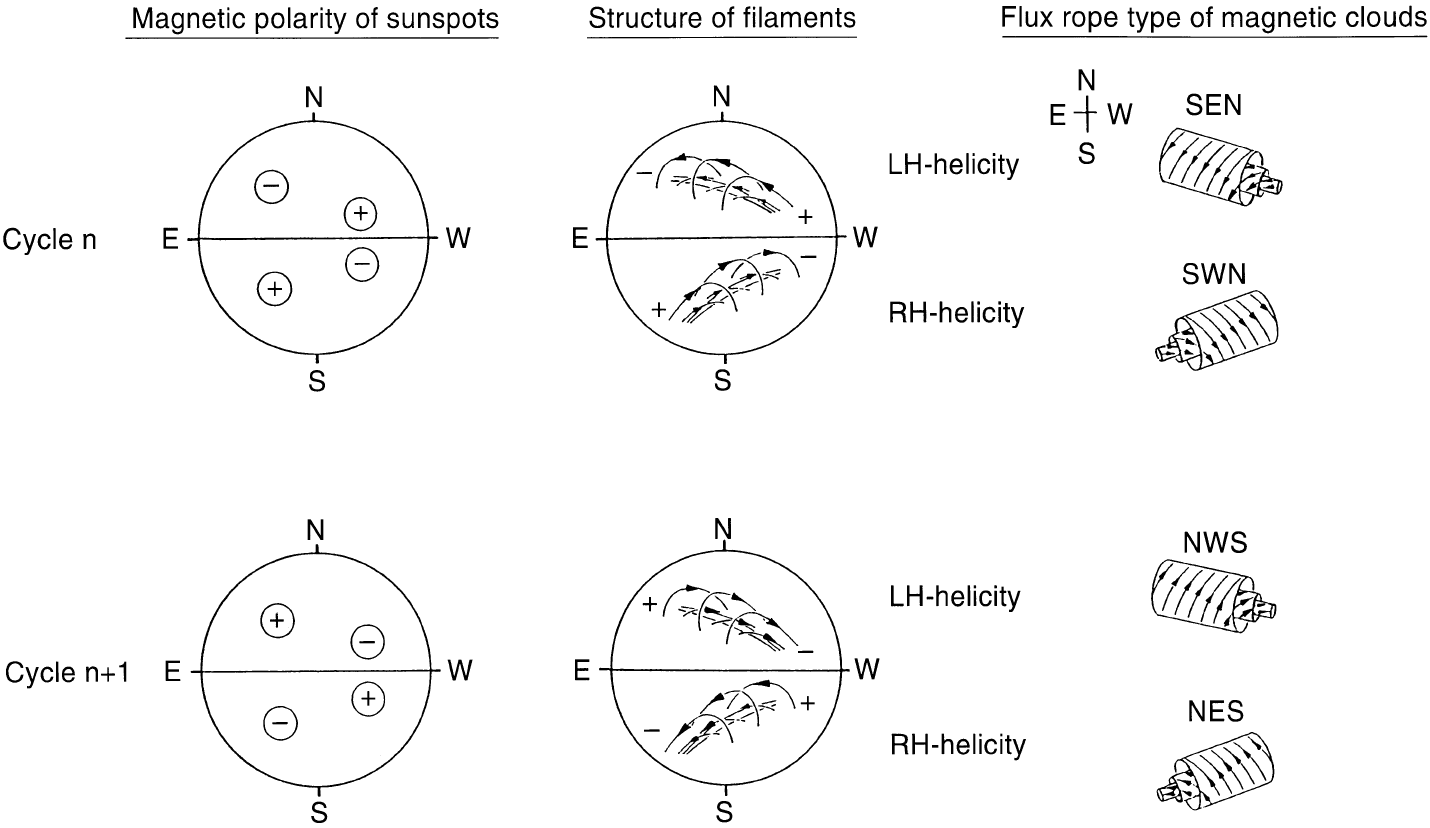
\includegraphics[width=\textwidth]{figures_of_others/images/Bothmer1998_fig18.png}
	\caption[\lofimage{figures_of_others/images/Bothmer1998_fig18.png}Credit: {\citet[Fig.~18]{Bothmer1998}}, \textcopyright~EGS -- Springer-Verlag, reproduced with permission.]
	{Explaining sketch of the BSS. The two rows represent odd ($n$) and even ($n + 1$) solar cycle numbers. The magnetic polarity of sunspots, the structure of filaments, their helicity, and the corresponding flux rope type of magnetic clouds are shown. Credit: {\citet[Fig.~18]{Bothmer1998}}, \textcopyright~EGS -- Springer-Verlag, reproduced with permission.}
	\label{fig:Bothmer1998_fig18}
\end{figure}
As the probability is greater than \SI{80}{\percent} that the magnetic topology of an active region conforms to the hemispheric rule \citep{Wang2013}, an MC configuration predicted with the BSS is expected to have a reliability that is of the same order \citep{Savani2015}.

% CME in-situ plot
Three CMEs can be seen in the solar wind in-situ measurements showed previously in \autoref{fig:ACE_64s_v7_thesis_CIRs_2013-5-1_65_plot}, passing by the ACE spacecraft at L1 on 24~May, 6~June, and 27~June in 2013. The latter CME has a well-structured MC, which is presented in detail in \autoref{fig:ACE_64s_v7_thesis_CME_2013-6-26_6} -- I use this event as an example throughout this section.
\begin{figure}[htb]
	\centering
	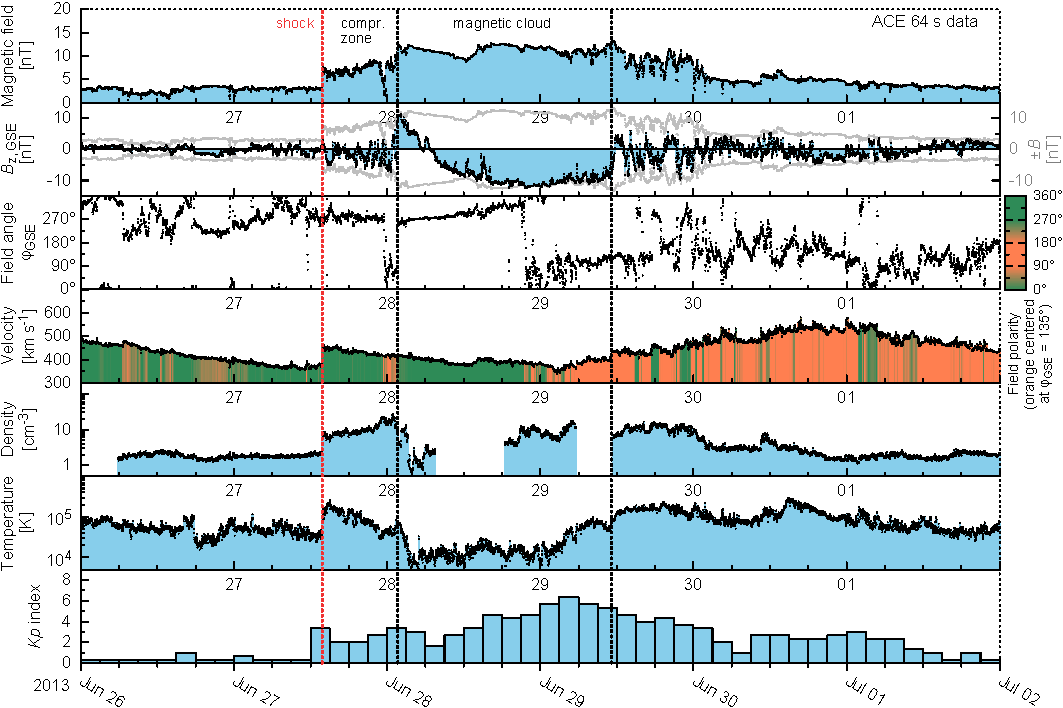
\includegraphics[width=\textwidth]{figures_of_mine/gnuplots/ACE_64s_v7_thesis_CME_2013-6-26_6.pdf}
	\caption[\lofimage{figures_of_mine/gnuplots/ACE_64s_v7_thesis_CME_2013-6-26_6.pdf}]
	{Solar wind with a CME, measured at L1 during the time period 26~June to 2~July in 2013. The solar wind parameters are the magnetic field strength, its z-component and ecliptic field angle in GSE~coordinates, the proton velocity, density, and temperature; in addition, the geomagnetic \Kp~index is plotted in the bottom panel. In the velocity panel also the field polarity is color coded -- assuming a fixed Parker spiral angle of \SI{135}{\degree}. I indicated the shock, the compression zone, and the duration of the magnetic cloud with dotted lines. Blank periods indicate bad or missing data. The solar wind data was measured with the MAG and SWEPAM instruments onboard the ACE spacecraft and is obtained from the ACE~Science~Center. The \Kp{}~data is obtained from the GFZ~Potsdam.}
	\label{fig:ACE_64s_v7_thesis_CME_2013-6-26_6}
	\addtocontents{lof}{\smallskip\protect\center I created the figure myself.\medskip}
\end{figure}
In addition to showing the solar wind in-situ parameters, I indicated the shock, compression zone and the MC with dotted lines, and plotted the geomagnetic \Kp{}~index in order to visualize the CME's impact on the magnetosphere. This MC contains a sector boundary and is trailed by an interaction region caused by a following HSS.

The CME occured in solar cycle~24. The MC's IMF z"~component changes from positive (northern) to negative (southern) values -- during this process, the field angle in the ecliptic, $\phi$, stays pointing roughly towards \SI{270}{\degree} (west). Thus, it has a NWS configuration, which is expected from the BSS during even numbered solar cycles for CMEs with source regions located in the northern hemisphere.

%white-light structure
The combination of white-light images with in-situ data enables relating the observed structures of CMEs. Even disturbances in front of fast CMEs can be identified as shock waves in the white-light images made by the SOHO coronagraph \citep{Sheeley2000}. The diffuse leading feature of a CME is the shock sheath, its brightness is caused by the density jump after the shock, which itself is not visible in coronagraphs. The trailing void is identical to the low density of the magnetic flux rope, which drives the whole structure.

The CME described before is indeed coming from the northern hemisphere, as can be seen from the STEREO~A coronagraph image displayed in \autoref{fig:STEREO_A_COR2_20130624_022400_dbc2A} taken three days earlier. Apparently, the CME only grazes the ecliptic and its lower part passes Earth. Also in this image, the event originates from the backside of the solar disk, considering the observing spacecraft's position in relation to Earth at that time, see \autoref{fig:STEREO_positions_w_269707595}.
\begin{figure}[htb]
	\begin{floatrow}
		\ffigbox{
			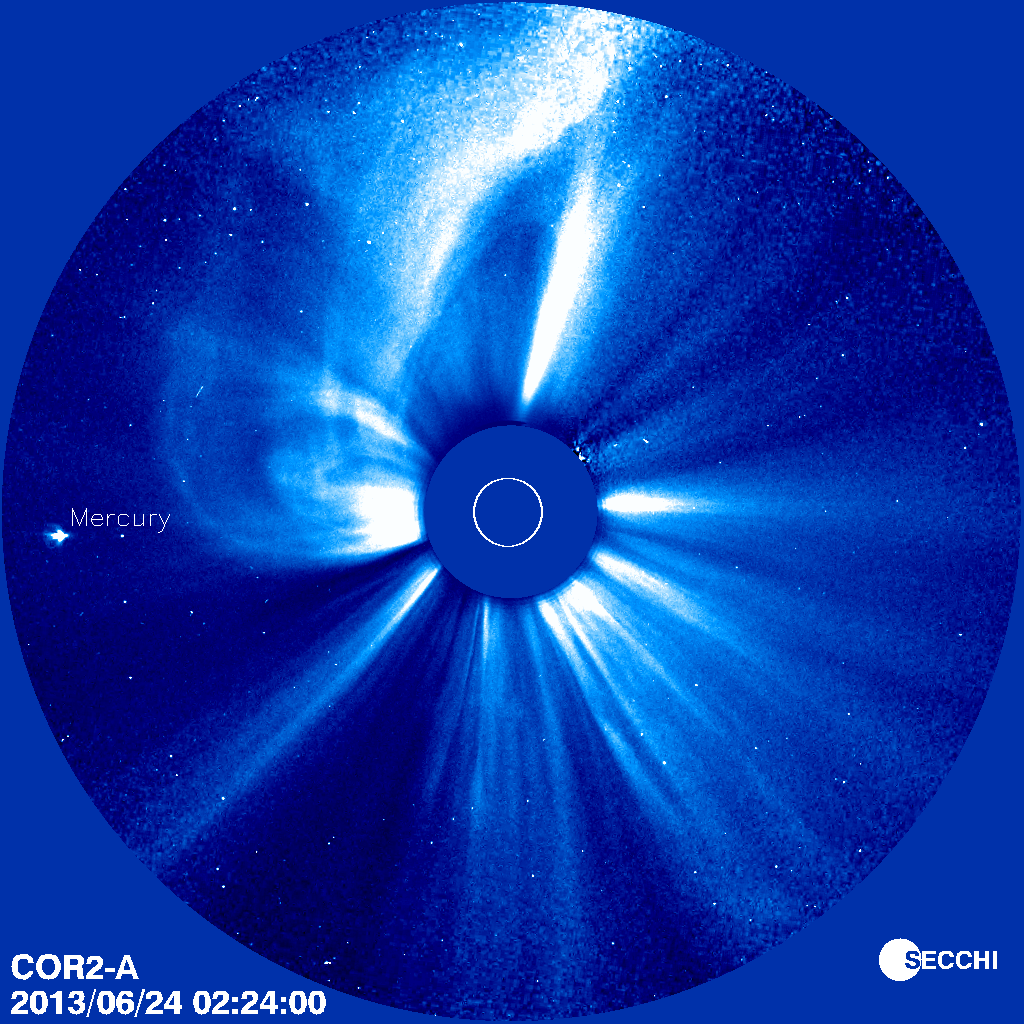
\includegraphics[width=0.45\textwidth]{figures_of_others/images/STEREO_A_COR2_20130624_022400_dbc2A.png}
		}{
			\caption[\lofimage{figures_of_others/images/STEREO_A_COR2_20130624_022400_dbc2A.png}Courtesy of \href{https://stereo.gsfc.nasa.gov/gallery/copyright.shtml}{STEREO/COR2 consortium (NASA)}.]
			{Image of the solar corona from 24~June 2013 made with the same coronagraph as the image in \autoref{fig:CME_COR2_0120923_182400_dbc2A}. The CME is the extended structure to the upper left. Courtesy of \href{https://stereo.gsfc.nasa.gov/gallery/copyright.shtml}{STEREO/COR2 consortium (NASA)}.}
			\label{fig:STEREO_A_COR2_20130624_022400_dbc2A}
		}
% https://secchi.nrl.navy.mil/sccimages/
% https://stereo-ssc.nascom.nasa.gov/browse/2013/06/24/index.shtml
		\ffigbox{
			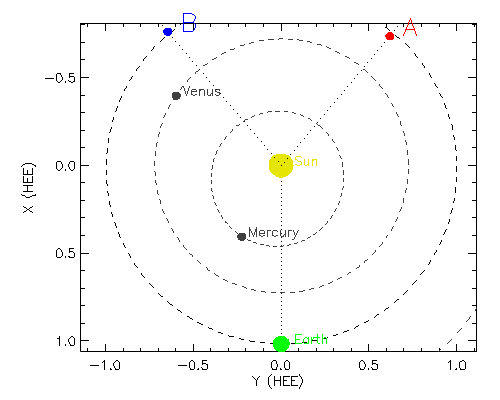
\includegraphics[width=\Xhsize]{figures_of_others/images/STEREO_positions_w_269707595.png}
		}{
			\caption[\lofimage{figures_of_others/images/STEREO_positions_w_269707595.png}]
			{Positions of the STEREO~A and~B spacecraft for 24~June 2013 02:24~UT. This figure is made with the online \href{https://stereo-ssc.nascom.nasa.gov/cgi-bin/make_where_gif}{STEREO Orbit Tool} at the STEREO Science Center website\protect\footnotemark.}
			\label{fig:STEREO_positions_w_269707595}
		}
% https://stereo-ssc.nascom.nasa.gov/cgi-bin/make_where_gif
	\end{floatrow}
\end{figure}
\footnotetext{STEREO Science Center website: \urlfoot{https://stereo-ssc.nascom.nasa.gov/}}

% CBS
Relating CME white-light images to observations of magnetic neutral lines on the solar surface, \citet{Cremades2004} interpreted the white-light appearances of CMEs as projections of their 3D geometry and developed a scheme for their orientation depending on the orientation and location of the neutral lines on the solar surface. Neutral lines on the solar surface are the lines of polarity inversion between two areas of opposite magnetic polarity. The scheme is based on the topology of the flux rope model and the observation that its major axis stays roughly aligned to the underlying neutral line during the eruption process. Thus, \citet{Cremades2004} concluded that CMEs look systematically different depending on their source region's position and magnetic configuration, as described in \autoref{fig:Cremades2004_fig15}.
\begin{figure}[htb]
	\centering
	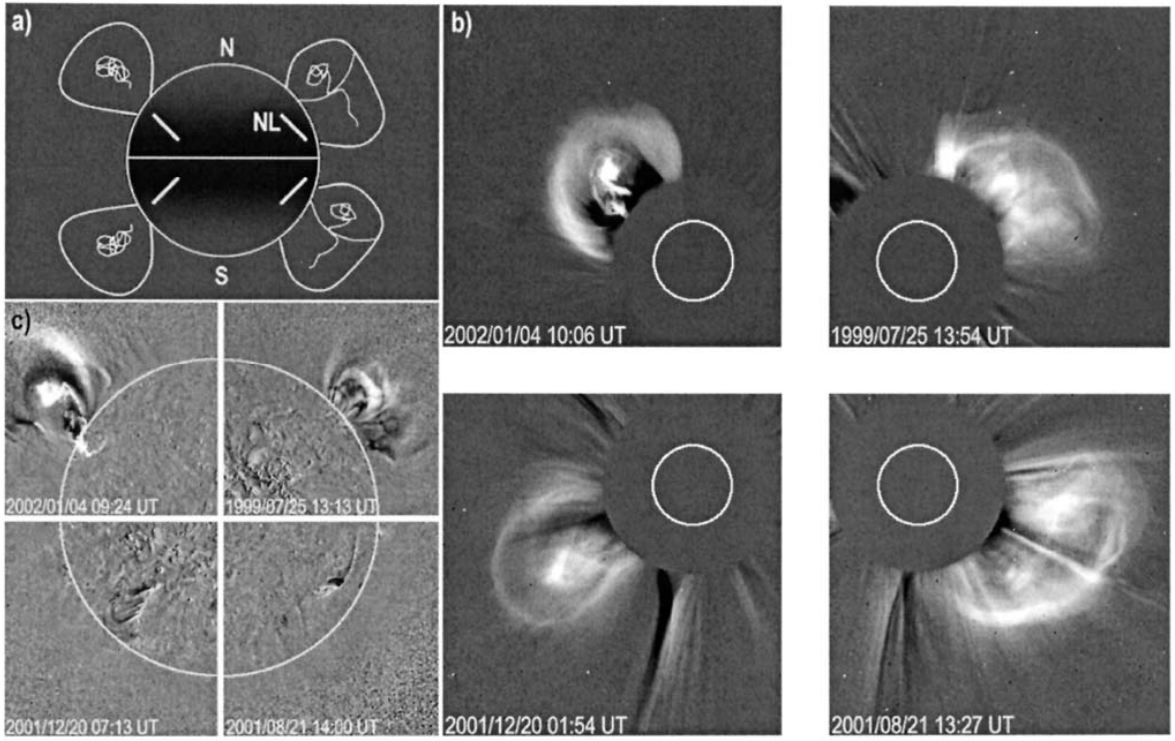
\includegraphics[width=\textwidth]{figures_of_others/images/Cremades2004_fig15.png}
	\caption[\lofimage{figures_of_others/images/Cremades2004_fig15.png}]
	{White-light CME projection scheme for frontside events, showing the case for each quadrant of the solar disk. (a)~Schema showing the expected white-light appearance of CMEs and the orientation of the underlying magnetic neutral lines. (b)~White-light images of CME example events, made with the LASCO C2 coronagraph on the SOHO spacecraft. (c)~Details (prominences and post-eruptive arcades) of the source regions related to the CMEs shown in panel~(b). Note that for events originating from the backside, panel~(a) has to be mirrored vertically. Credit: {\citet[Fig.~15]{Cremades2004}}, \textcopyright~ESO, reprinted with permission.}
	\label{fig:Cremades2004_fig15}
\end{figure}
For the solar backside, the neutral lines are reversed and according to the scheme so are the CME orientations -- thus the broad backside CME seen in \autoref{fig:CME_COR2_0120923_182400_dbc2A} matches this scheme. The scheme can effectively be applied for CMEs with source regions located less than \SI{50}{\degree} from the solar equator \citep{Webb2012}.

This white-light CME projection scheme as well as the BSS for MCs are based on the notion that the orientation of flux ropes propagating outwards generally stays aligned with the neutral polarity inversion line on the solar surface where the filament erupted \citep{Marubashi1997,Bothmer1998}. In fact, it is shown that flux ropes are not likely to rotate significantly after their initiation but maintain the orientation of their main axis parallel to the magnetic neutral line even in interplanetary space \citep{Marubashi2015}. However, during and shortly after their eruption, CMEs are frequently observed to be deflected to other directions by the surrounding coronal magnetic field structure \citep{Sterling2011}.

% CME redefinition
The revelation that all CMEs may be flux ropes \citep{Vourlidas2013,Marubashi2015} led to the expansion of the CME definition based on white-light images made by \citet{Hundhausen1984}. \citet{Vourlidas2013,Vourlidas2014} include magnetic flux ropes in their recent CME redefinition: \textit{``A CME is the eruption of a coherent magnetic, twist-carrying coronal structure with angular width of at least \SI{40}{\degree} and able to reach beyond \SI{10}{\Rs} which occurs on a time scale of a few minutes to several hours.''}

% flux rope distortion
However, CMEs generally do not have a perfect flux rope geometry: Often their more complex structure can be seen in kinks of the corresponding filament before the eruption; and strong distortions can happen during the eruption process. Their cross section is only initially of circular shape, it distorts due to the pressure-driven self-expansion and the radial solar wind expansion \citep{Owens2006}. Though, the inner core of the flux rope is believed to stay of circular shape. For these reasons, the properties of CMEs vary widely and imaging projection effects contribute further to that \citep{Cremades2004}.

%open questions
There still exist a lot of unresolved questions about CMEs, their formation, and the effects observed along with them: Multiple mechanisms/processes are debated for the release of CMEs and their subsequent acceleration. It is also not known if there exist CMEs without magnetic flux ropes \citep{Vourlidas2013}. The relation between flux ropes observed in the near-Sun corona and measured in~situ at interplanetary distances is still not entirely clear \citep{Vourlidas2014}. Nobody knows yet when a CME will erupt on the Sun, at what exact time it will pass a given point in the heliosphere, and how its detailed magnetic configuration would look like in~situ \citep{Gopalswamy2016}.\\


%white-light images of a backside CME\\
% SOHO LASCO CME CATALOG
% 2013/06/24 	04:00:05 	Halo 	
% https://cdaw.gsfc.nasa.gov/CME_list/UNIVERSAL/2013_06/univ2013_06.html
% https://cdaw.gsfc.nasa.gov/movie/make_javamovie.php?stime=20130624_0236&etime=20130624_0714&img1=lasc2rdf&title=20130624.040005.p235g;V=709km/s


% % CBS
% Using SOHO LASCO, EIT, and MDI and ground-based H$\alpha$ data,  \citet{Cremades2004} concluded that a simple scheme can be used to relate CME white-light topology to the heliographic position and orientation of the underlying magnetic neutral line.\\
% When the neutral line is approximately parallel to the solar limb, the CME appears as a linear feature parallel to the limb having a broad, diffuse inner core. When the neutral line is approximately perpendicular to the solar limb, the CME is observed along its symmetry axis, and the core material lies along the line of sight. Joy’s law implies that the frontside neutral line will typically lie perpendicular to the east limb and parallel to the west limb. from \citep{Webb2012}.\\
% 
% The real axis of the CME seems to correspond with the long axis of a large-scale helical magnetic flux rope that was formed in the SR, with the prominence being the bottom part of this magnetic system \citep{Cremades2004}.\\
% 
% Sun Earth Connection Coronal and Heliospheric Investigation (SECCHI) on board the Solar Terrestrial Relations Observatory (STEREO) spacecrafts \citep{Howard2008}\\



% literature:
% historical CME review by \citet{Gopalswamy2016}.\\
% historic review; Syun-Ichi Akasofu2011\\


\section{Space weather}
\label{sec:space_weather}
Space weather is the field of research that comprises all dynamic effects generated by the Sun in its domain of influence -- the heliosphere. Naturally, it is especially focused on the solar effects observed on Earth and in its local environment -- the ionosphere and the magnetosphere. There exist several different effects caused by independent solar events occurring on different time scales that can affect humans directly or indirectly. Solar events affect sensitive technical systems and strong events are even able to disrupt them and pose a threat to humans \citep{Bothmer2007}. Space weather deals with effects on time scales similar to the terrestrial weather, that is, days and weeks.

The existence of a direct solar-terrestrial relation was known of early on. \citet{Carrington1859} made the first connection between solar flares and disturbances in the terrestrial magnetic field when he observed a brightening on the solar disk on 1~September 1859 and suggested its connection to a strong geomagnetic storm that occurred about 17~hours later. Categories of solar-terrestrial correlations were already listed by \citet{Bartels1962}: Events initiated by irregular solar X"~ray flares and CMEs, by the 11"~year solar activity cycle, and by the periodic 27"~day solar rotation. Other time related variations include seasonal effects caused by the Earth's orbital distance oscillation over the year and the inclinations of the Sun's and Earth's rotation axes to the ecliptic normal. The terrestrial magnetic field's dipole axis tilt to the rotation axis further contributes to the daily effects.

The major driving forces behind severe space weather events are CMEs, solar X"~ray flares, and solar energetic particle (SEP) events. Most of the terrestrial space weather effects are introduced through the events' influence on the magnetosphere, ionosphere, and upper atmosphere. Space weather effects are commonly classified into geomagnetic storms, solar radiation storms, and radio blackouts\footnote{NOAA Space Weather Scales website: \urlfoot{https://www.swpc.noaa.gov/noaa-scales-explanation}}.

The solar wind's internal structures, such as CMEs and CIRs, affect the magnetosphere and can cause disturbances in its magnetic field, such as geomagnetic storms and substorms, both are described in more detail in the following section. Notable consequences of these disturbances in the terrestrial magnetic field are listed below \citep{Bothmer2007}:
\begin{itemize*}
	\item Impact on the magnetic navigation and behavior of animals, such as migratory birds \citep{Moore1977} and whales \citep{Vanselow2017}.
	\item Enhanced auroral activity and shift of the auroral oval to lower latitudes\footnote{NOAA/SWPC Tips on Viewing the Aurora: \urlfoot{https://www.swpc.noaa.gov/content/tips-viewing-aurora}}.
	\item The equatorward auroral oval shift leads to direct risks for humans from enhanced radiation doses during high altitude flights through the enlarged polar cap\footnote{NOAA/SWPC Galactic Cosmic Rays: \urlfoot{https://www.swpc.noaa.gov/phenomena/galactic-cosmic-rays}}.
	\item Enhanced radiation in the Van~Allen belt can lead to faulting electronics and disturb satellite operations.
	\item Geomagnetic storms can rapidly heat the upper atmosphere, causing it to expand, and generate an increased drag for satellites in low Earth orbits\footnote{NOAA/SWPC Satellite Drag: \urlfoot{https://www.swpc.noaa.gov/impacts/satellite-drag}}.
	\item Geomagnetically induced currents are created in long conducting infrastructure, such as oil pipelines, rail tracks, and power lines. The currents can lead to increased steel corrosion and power grid outtages.
	\item The sunward magnetopause distance can shrink under extreme solar wind pressure below the geostationary Earth orbit (GEO) at a distance of \SI{6.6}{\RE}. GEO satellites crossing the magnetopause are then directly exposed to the radiation of SEPs.
\end{itemize*}

Solar extreme ultraviolet (EUV) and X"~ray radiation events affect the ionosphere apart from their regular day/night cycle influence. Solar flares can create sudden ionospheric disturbances \citep{Gosling1993}, that is, abrupt enhancements in the ionospheric total electron content (TEC). These TEC variations threaten the following technical systems \citep{Kraaikamp2015}:
\begin{itemize*}
	\item Increased TEC leads to larger positioning errors in global navigation satellite systems (GNSS).
	\item Scintillation and absorption of high frequency signals on their way through the ionosphere can lead to signal disturbances and loss of satellite communications.
	\item Induced changes in the stratification of the ionosphere (D-, E-, and F"~layers) disturb radio communication and lead to outtages in different frequencies.
\end{itemize*}

Flares and CME shock fronts accelerate coronal particles, producing SEPs. High fluxes of SEPs induce solar radiation storms with durations ranging from hours to days that have the following effects \citep{Bothmer2007}:
\begin{itemize*}
	\item Enhanced radiation damage to electronic circuits in satellites and spacecraft.
	\item Enhanced radiation damage to biological tissue in humans and all organisms brought to space.
	\item SEPs are guided by the terrestrial magnetic field down to the polar regions. Humans flying in aircraft near polar latitudes are exposed to higher radiation doses during strong radiation storms. Especially humans in orbit outside the protective atmosphere are endangered.
	\item Free electrons, created by SEPs colliding with the atmosphere, form ionospheric layers that disturb/block high frequency radio communications\footnote{NOAA/SWPC Solar Radiation Storm: \urlfoot{https://www.swpc.noaa.gov/phenomena/solar-radiation-storm}}.
\end{itemize*}

There exist lots of space weather effects on the rest of the solar system bodies. Notable effects are \citep{Bothmer2007}:
\begin{itemize*}
	\item Solar wind structures can strip off cometary tails and can enhance atmospheric losses in bodies without magnetosphere.
	\item Other planetary magnetospheres are impacted in similar ways as the terrestrial is (e.g., the Jovian and Saturnian magnetospheres).
	\item Induced magnetospheres on nonmagnetic bodies, as is the case at Venus, are affected by the varying external plasma of the solar wind \citep{Luhmann2004}.
	\item The average solar wind pressure and HMF scale with solar activity and therefore modulate the shape and size of the heliosphere. As cosmic rays are influenced by the HMF, the local cosmic ray radiation level scales inversely with solar activity. Even the passing of strong MCs lead to reductions in local cosmic ray radiation, which are called Forbush decreases.
	\item The solar system regions outside of protective magnetospheres suffer directly from episodes of enhanced solar radiation.
\end{itemize*}

As can be seen, most terrestrial space weather effects are connected with economic interests and some impacts on technical systems can even influence human lives. This creates a strong interest in forecasting the space weather conditions. Space weather forecasting is a relatively new field of study, however, it becomes more and more important, not only because of the increasing use of sensitive technology at Earth, but also because of the anticipated expansion of interplanetary space activities within the near future, such as human space missions to Moon or Mars. There exist lots of dedicated institutions and a multitude of forecasting techniques for the different aspects of space weather and more are being developed.

Predictions of magnetospheric disturbances are based on knowledge of the solar wind properties, which the magnetosphere will encounter. Thus in a first step, forecast methods have to predict the solar wind at Earth in advance and derive its expected impact on the magnetosphere in a second step. The first part of this present study contributes to the second step with predicting the amplitude of magnetospheric disturbances caused by solar wind. The basic structure of the magnetosphere, its coupling to the solar wind, and how disturbances are quantified/measured is described in the following \autoref{sec:magnetosphere}. Existing forecast methods for geomagnetic disturbances and for their solar wind sources are described in \autoref{sec:forecast_methods}.


\section{Magnetosphere}
\label{sec:magnetosphere}
In first-order approximation, the terrestrial magnetic field can be seen as a dipole aligned with the rotation axis of the Earth. Its magnetic south pole is located near the geographic North Pole and there is currently only a small tilt of about \SI{9.5}{\degree} between both axes \citep{Thebault2015} -- it varies slightly over the years. The magnetic field strength on the surface at the poles is around \SI{60}{\micro\tesla}, whereas at the equator it is about half that magnitude. At the Earth's surface, this dipole approximation neglects major field irregularities, such as the prominent South Atlantic Anomaly whose field is lower than \SI{24}{\micro\tesla} \citep{Thebault2015}.

The geomagnetic field's strength decreases while it extends out into space. Its influence ends where its magnetic pressure balances the ram pressure of the solar wind. \citet{Gold1959} named the region governed by the terrestrial magnetic field the magnetosphere. The outer boundary is the magnetopause -- in average it has a sunward distance of about \SI{11.0}{\RE} \citep{Fairfield1971}. In response to the continuous changes in the solar wind pressure, the magnetopause usually is in a state of fast radial inward-outward motion and its displacement can reach several Earth radii \citep{DeKeyser2005}. The solar wind flow shapes the magnetopause into a surface of teardrop form, whose so-called magnetotail length varies around \SI{100}{\RE} and points away from the Sun.

The solar wind compression at the front of the magnetopause creates a bow shock, whose average standoff distance to Earth is about \SI{15.1}{\RE} but varies largely under extreme solar wind conditions \citep{Fairfield1971}. The shocked solar wind plasma flows within the magnetosheath around the magnetosphere as seen in \autoref{fig:Davies1990_magnetosphere_sharpened}.
\begin{figure}[htb]
	\fcapside[\FBwidth]{
		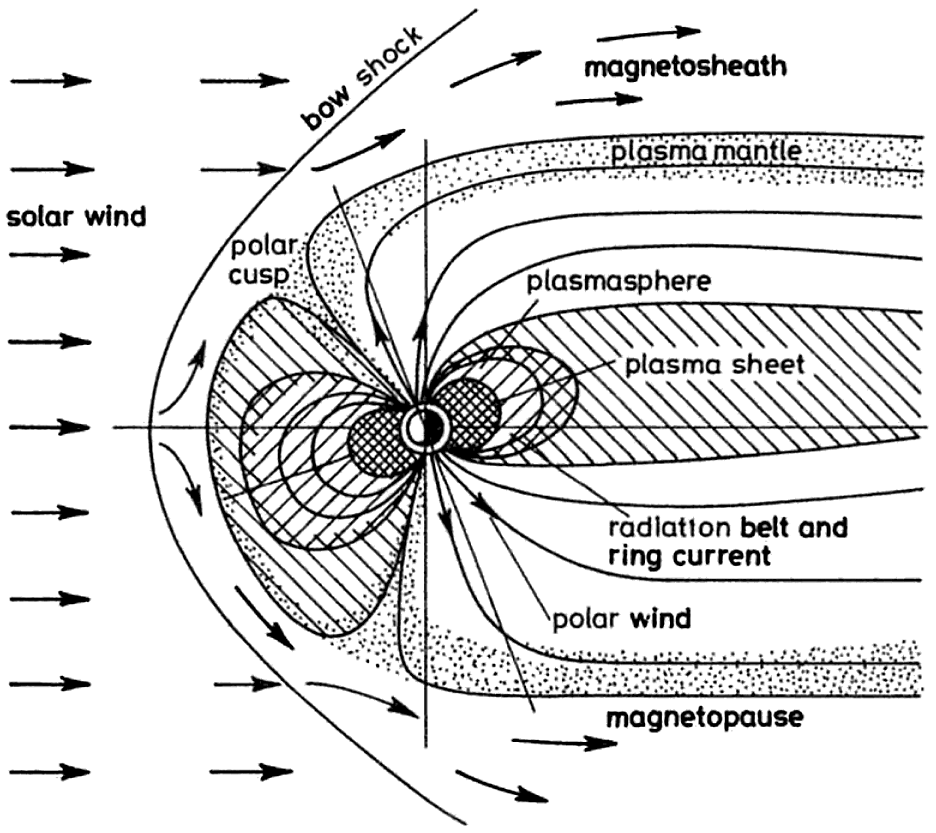
\includegraphics[width=0.6\textwidth]{figures_of_others/images/Davies1990_magnetosphere_sharpened.png}
	}{
		\caption[\lofimage{figures_of_others/images/Davies1990_magnetosphere_sharpened.png}]
		{Schema of the magnetosphere's geometry in the plane spanned by the solar wind flow direction and the ecliptic normal (vertical line). The arrows show the flow of solar wind around the Earth's magnetic field. The diagonal line indicates the inclination of the rotation axis to the ecliptic. Credit: {\citet[Fig.~2.12]{Davies1990}}, \textcopyright~IET, ... get permission...}
		\label{fig:Davies1990_magnetosphere_sharpened}
	}
\end{figure}
% http://digital-library.theiet.org/content/books/ew/pbew031e
The IMF in the magnetosheath is weaker but has a larger variability than the terrestrial magnetic field on the other side of the magnetopause \citep{DeKeyser2005}.

At the front of the magnetopause, the incoming solar wind ions and electrons are being deflected in direction of dawn and dusk by the magnetospheric field, creating a current layer at the surface of the magnetopause. This current induces another magnetic field that cancels the geomagnetic field outside of the magnetopause and enhances it inside to about twice the strength of a pure dipole field at that distance \citep{DeKeyser2005}. At the magnetotail side, the magnetopause current flows into the opposite direction -- an overview, also of the inner magnetosphere's current systems is illustrated in \autoref{fig:DeKeyser2005_magnetosphere}.
\begin{figure}[htb]
	\fcapside[\FBwidth]{
		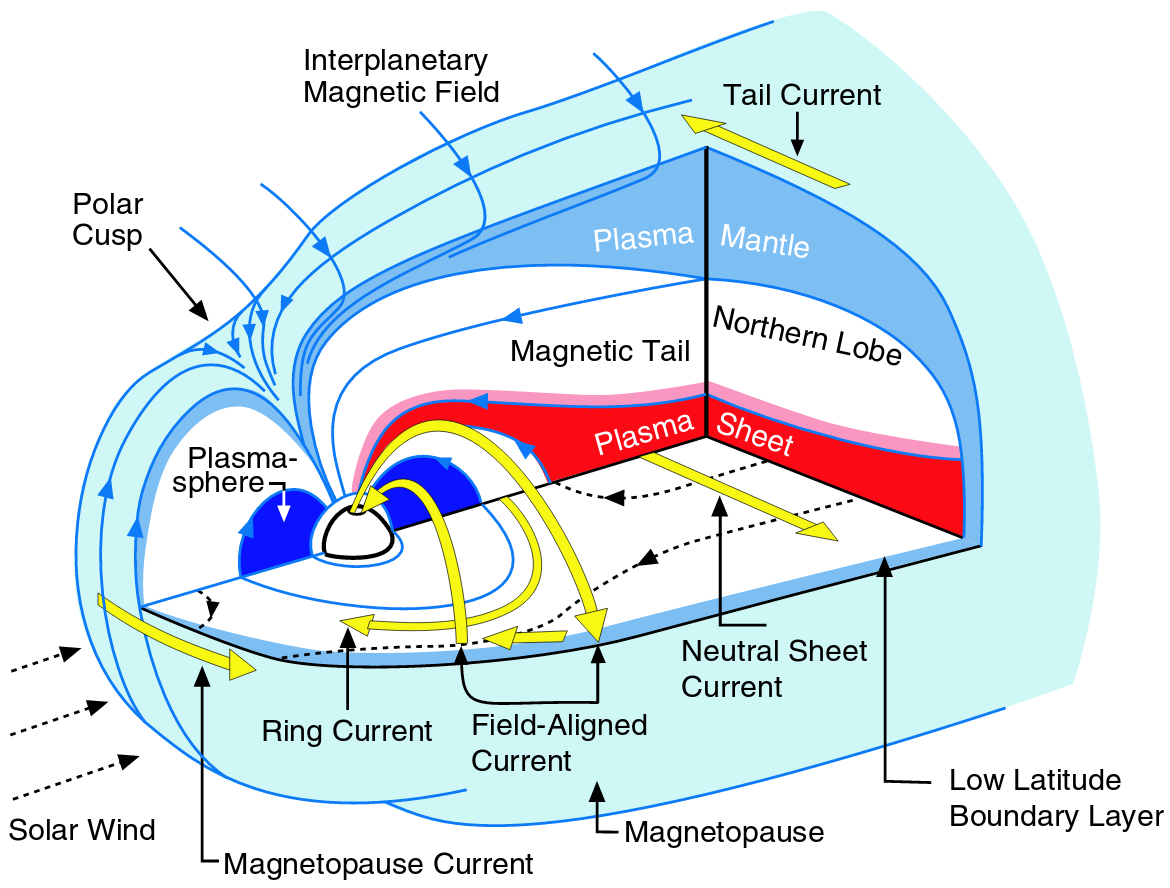
\includegraphics[width=0.6\textwidth]{figures_of_others/images/DeKeyser2005_magnetosphere.png}
	}{
		\caption[\lofimage{figures_of_others/images/DeKeyser2005_magnetosphere.png}]
		{Schema of the magnetosphere's inner 3D structure with focus on its current systems and plasma regions. The directions of the magnetic field lines and electric currents are indicated with blue and yellow arrows. Credit: {\citet[Fig.~2.12]{DeKeyser2005}}, adapted from {\citet[Fig.~1.18]{Kivelson1995}}, \textcopyright~Springer, reproduced with permission.}
		\label{fig:DeKeyser2005_magnetosphere}
	}
\end{figure}


\subsection{Solar wind coupling mechanisms}
\label{sec:solar_wind_coupling}
There exist several ways of how solar wind couples to the magnetosphere and deposits energy and plasma within. The contributions of the different mechanisms by which energy is transferred and solar wind plasma is able to penetrate the magnetopause are not yet established \citep{Phan2005}. High solar wind pressure during times when the IMF direction is parallel to the terrestrial magnetic field leads to compression of the sunward magnetosphere and enhances its potential energy. Solar wind energy is also transferred via the induction of currents. However, the major interaction processes are magnetic reconnection and turbulence, their underlying physical mechanisms are described in the following.

Magnetic reconnection occurs where the IMF comes into antiparallel contact with the terrestrial magnetic field. At these regions on the magnetopause, the magnetosphere opens up to the IMF and reconnection of the field lines occurs, resulting in a change of the local magnetic topology \citep{Phan2005}. The oppositely directed magnetic field lines reconnect along a line that shows an X"~geometry. The reconnection process at this so-called X"~line harbors a narrow diffusion region, where the plasma ions and electrons decouple to get accelerated in jets of particles by the reconnected field lines \citep{Phan2005}, see the \autoref{fig:NASA_reconnection}.
\begin{figure}[htb]
	\fcapside[\FBwidth]{
		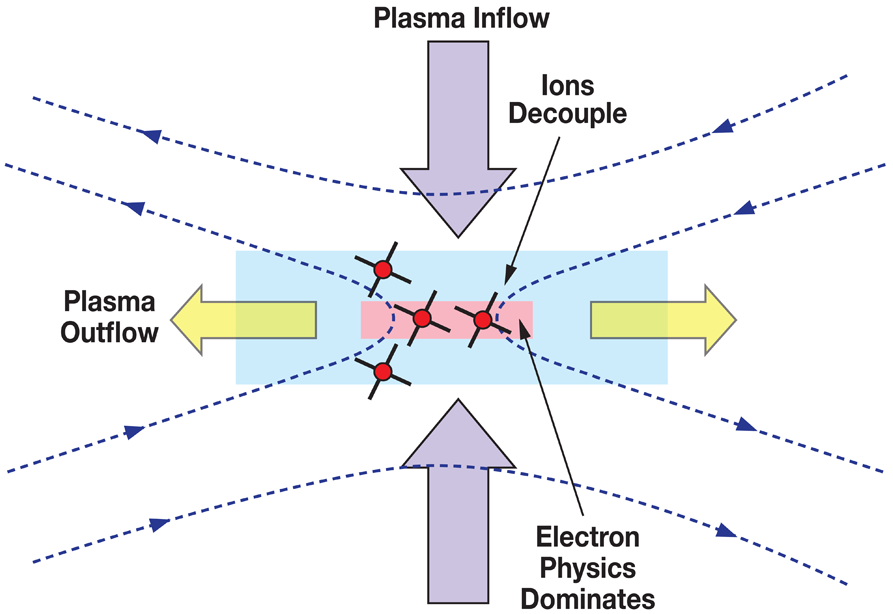
\includegraphics[width=0.5\textwidth]{figures_of_others/images/NASA_reconnection.png}
	}{
		\caption[\lofimage{figures_of_others/images/NASA_reconnection.png}]
		{Schema of an X"~line reconnection region. The dashed arrowed lines represent magnetic field lines and their direction. The large arrows indicate the plasma flow direction and the shaded areas are the ion and electron diffusion regions. The red crosses represent four Magnetospheric Multiscale (MMS) spacecraft that are built to analyze the magnetopause reconnection. Credit: \href{https://mms.gsfc.nasa.gov/science.html}{NASA/GSFC MMS mission}.}
		\label{fig:NASA_reconnection}
	}
\end{figure}
% https://mms.gsfc.nasa.gov/images/science_page/science_2_lg.png
% https://mms.gsfc.nasa.gov/science.html
Thus, the magnetopause is left with a small magnetic field normal to it that has an opposite polarity on each side of the X"~line \citep{DeKeyser2005}.

The reconnection location on the magnetopause shifts depending on the direction of the incoming IMF. During periods of southern IMF, the terrestrial field and IMF are antiparallel at the sunward point of the magnetosphere, owing to the Earth's dipole orientation. The rate of reconnection becomes highest in this case, whereas, when the IMF is directed northward, reconnection tailward of both polar cusps has been observed \citep{Phan2005}. The magnetic flux opened at the front of the magnetosphere is in average balanced by reconnections in the magnetotail, closing the field again. This process is part of the Dungey convection cycle which is described in the next \autoref{sec:dungey_convection_cycle}.

Although the microphysical processes leading to magnetic reconnection are yet little understood \citep{Phan2005}, there is evidence that magnetic reconnection is the dominant plasma transport mechanism into the magnetosphere \citep{DeKeyser2005}.

Viscous interaction with the solar wind plasma is also able to insert energy into the magnetosphere \citep{Alfven1942}. Solar wind drag at the flanks of the magnetopause creates Kelvin-Helmholtz (KH) instabilites in form of turbulent eddies. It is observed that even during northern IMF, these turbulent vortices are able to channel solar wind plasma into the magnetosphere -- either through forced magnetic reconnection (see \autoref{fig:Merkin2013_fig5_turbulence}) or non-reconnection processes \citep{Otto2003,Phan2005}. MHD simulations of the velocity shear at the magnetopause during northern IMF even suggest the presence of a double-vortex sheet structure \citep{Merkin2013}.
\begin{figure}[htb]
	\fcapside[\FBwidth]{
		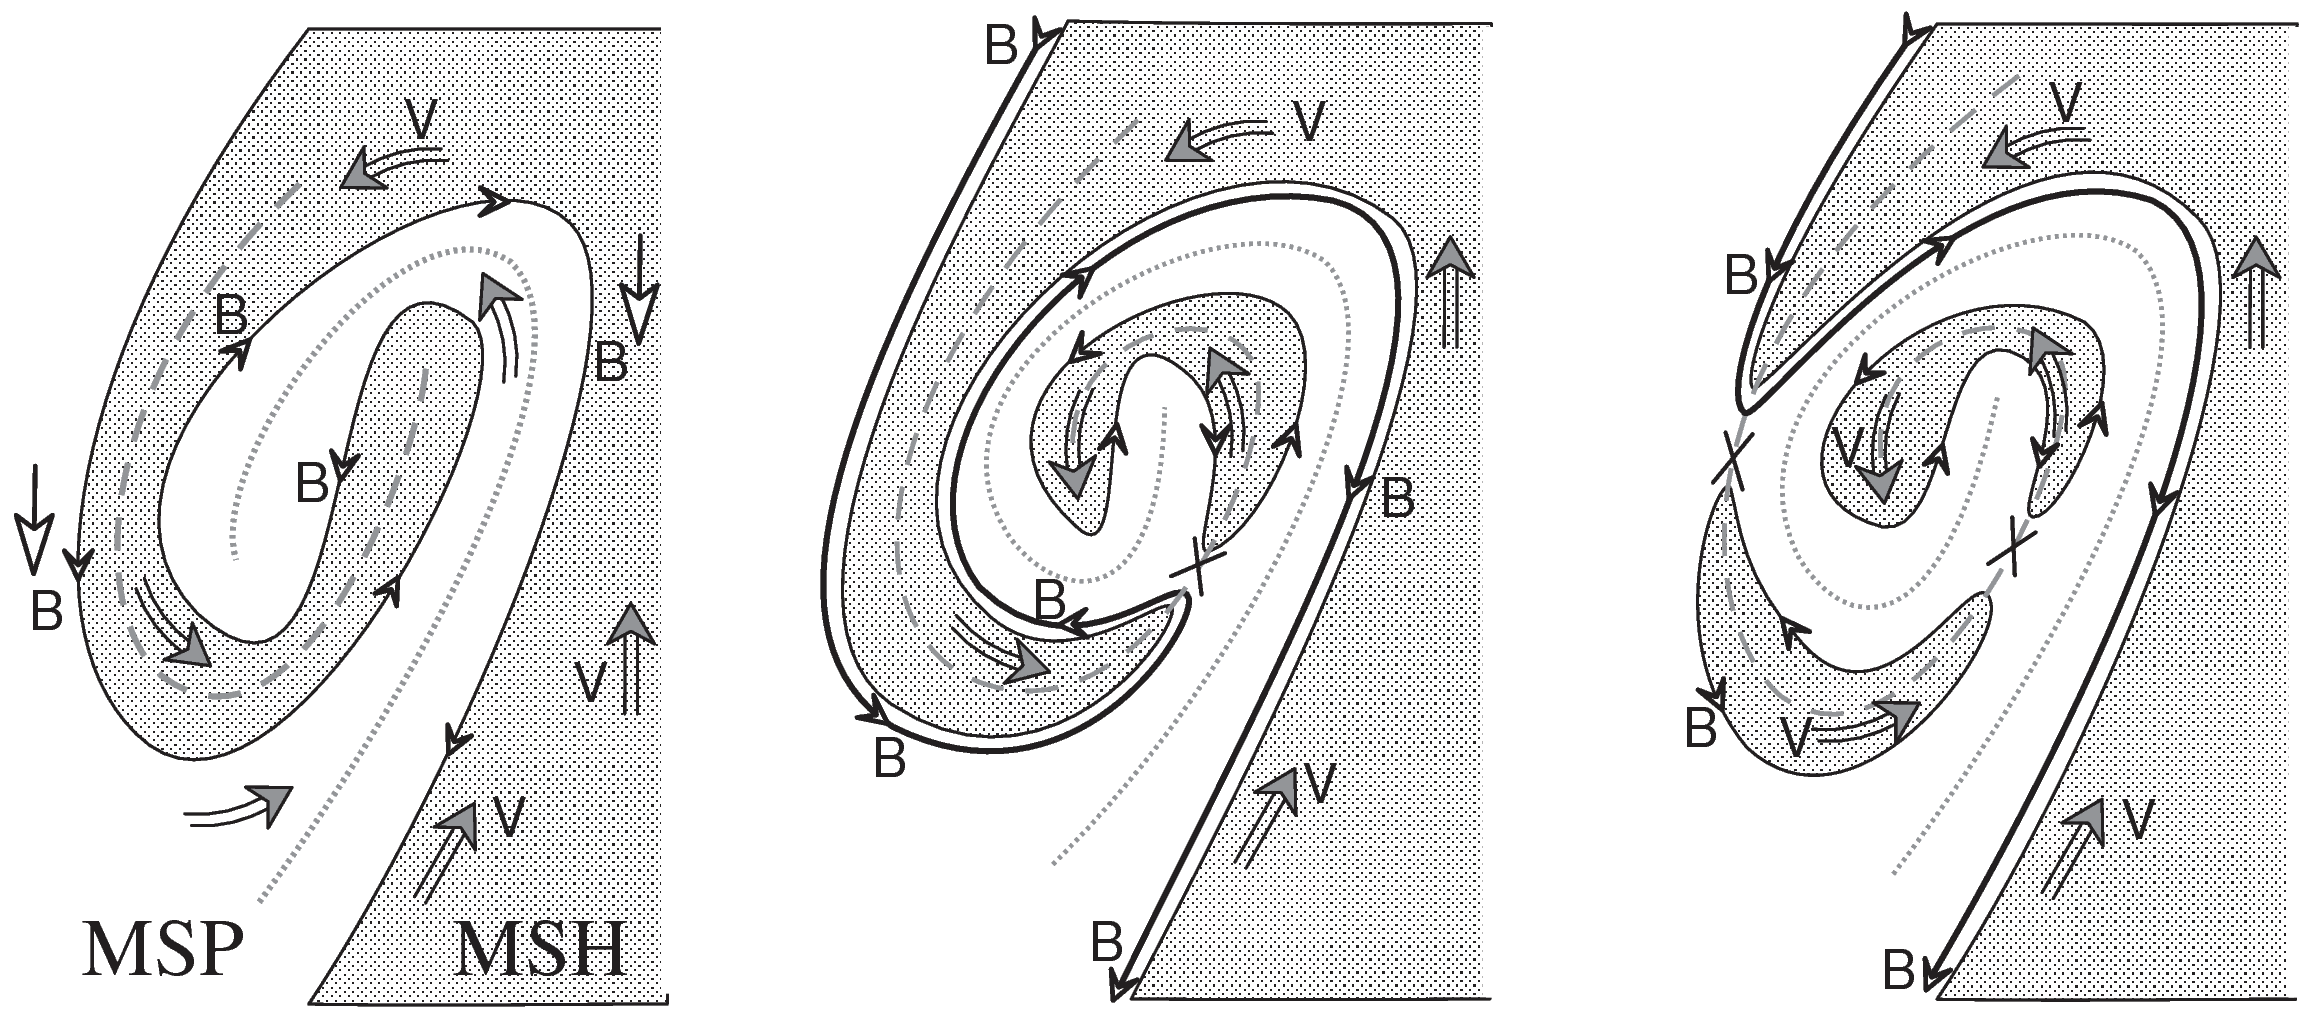
\includegraphics[width=0.6\textwidth]{figures_of_others/images/Merkin2013_fig5_turbulence.png}
	}{
		\caption[\lofimage{figures_of_others/images/Merkin2013_fig5_turbulence.png}]
		{Schemata showing reconnection in a turbulent vortex, forming between the magnetosphere (MSP) and the magnetosheath (MSH, shaded area) when both magnetic fields are parallel. The boundary magnetic field line is indicated by the arrowed line, the plasma flow direction by the gray arrows, and the locations of reconnection by crosses. Credit: {\citet[Fig.~5]{Merkin2013}}, \textcopyright~American Geophysical Union, reproduced with permission.}
		\label{fig:Merkin2013_fig5_turbulence}
	}
\end{figure}


\subsection{Dungey convection cycle}
\label{sec:dungey_convection_cycle}
% Dungey convection cycle
After the reconnection at the sunward magnetopause, the previously closed magnetospheric field lines are open to the IMF. They are still connected to one of the poles, but their IMF part is transported by the flow of the solar wind. The field lines are stretched behind Earth and form eventually the extended magnetotail, where in its central plane reconnection recloses the field. The closed field lines migrate around the flanks of the magnetosphere to its front again, completing one magnetic convection cycle \citep{Dungey1961,Dungey1963}. The course of this so-called Dungey convection cycle induced by the solar wind is illustrated in \autoref{fig:Kivelson1995_fig9_11_dungey_cycle}. The Dungey cycle imprints a twin-cell convection pattern in the high latitude ionospheric plasma, where the footpoints of the geomagnetic field lines are swept from the day- to the nightside and wander back again along the lower latitudes of dusk and dawn.
\begin{figure}[htb]
	\fcapside[\FBwidth]{
		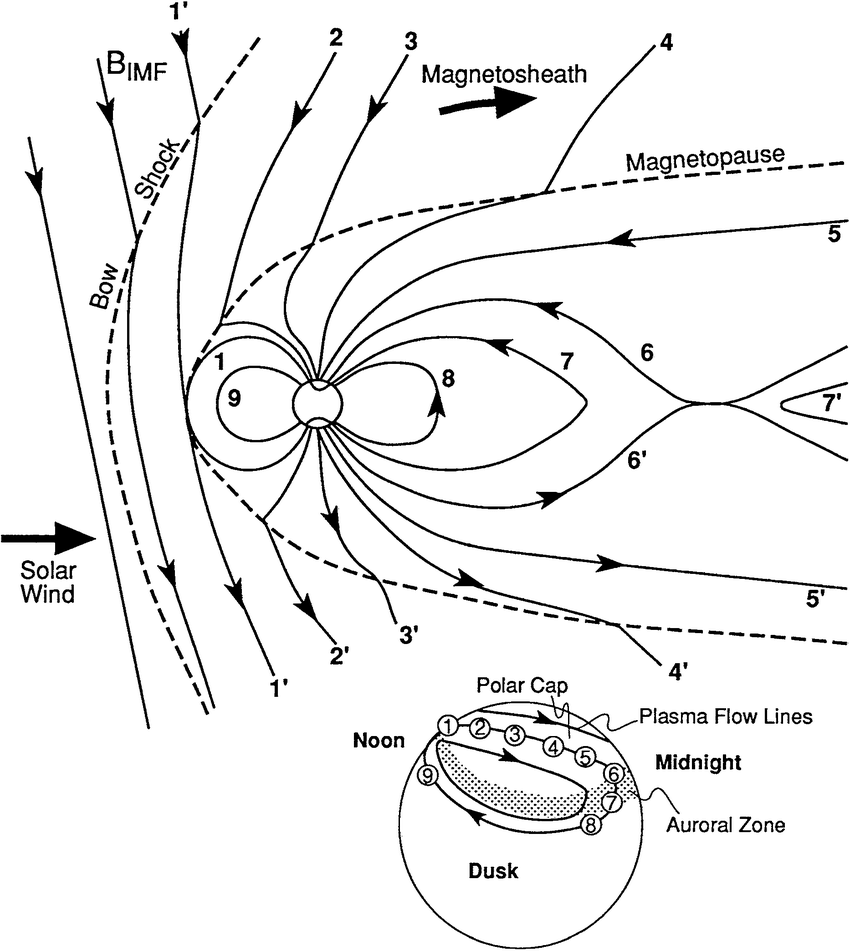
\includegraphics[width=0.6\textwidth]{figures_of_others/images/Kivelson1995_fig9_11_dungey_cycle.png}
	}{
		\caption[\lofimage{figures_of_others/images/Kivelson1995_fig9_11_dungey_cycle.png}]
		{Dungey's magnetic convection cycle illustrated in a cut through the magnetosphere (top) and on the ionosphere polar cap (bottom). The numbers on the magnetic field lines (arrowed lines) correspond to the numbered positions in the twin-cell polar cap convection cycle. Credit: {\citet[Fig.~9.11]{Hughes1995}}, \textcopyright~Cambridge University Press, reproduced with permission.}
		\label{fig:Kivelson1995_fig9_11_dungey_cycle}
	}
\end{figure}

% auroral ovals
Reconnection at the magnetopause releases and accelerates the local plasma from the reconnection site along the magnetic field lines. Thus, this plasma reaches the field lines' polar footpoints and interacts with the atoms and molecules of the upper atmosphere, creating the aurorae. The auroral ovals are located at the boundaries between the closed terrestrial field and the field open to the IMF. The open field regions, enclosed by the auroral ovals, are the polar caps. The increased reconnection during southward IMF erodes the magnetopause \citep{Aubry1970}, shifting the auroral ovals to lower latitudes. Likewise, the azimuthal IMF component shifts the auroral oval towards dawn or dusk.

The Dungey cycle is not a steady-state process, that is, the rates of opened and reclosed terrestrial magnetic flux are equal only in the long term. The dayside opening flux rate $\Phi_\text{D}$ is modulated by the dynamic behavior of the solar wind and the orientation of the IMF, whereas the nightside closing flux rate $\Phi_\text{N}$ depends on the situation in the magnetotail \citep{Milan2007}, see \autoref{fig:Milan2009_magnetosphere}.
\begin{figure}[htb]
	\fcapside[\FBwidth]{
		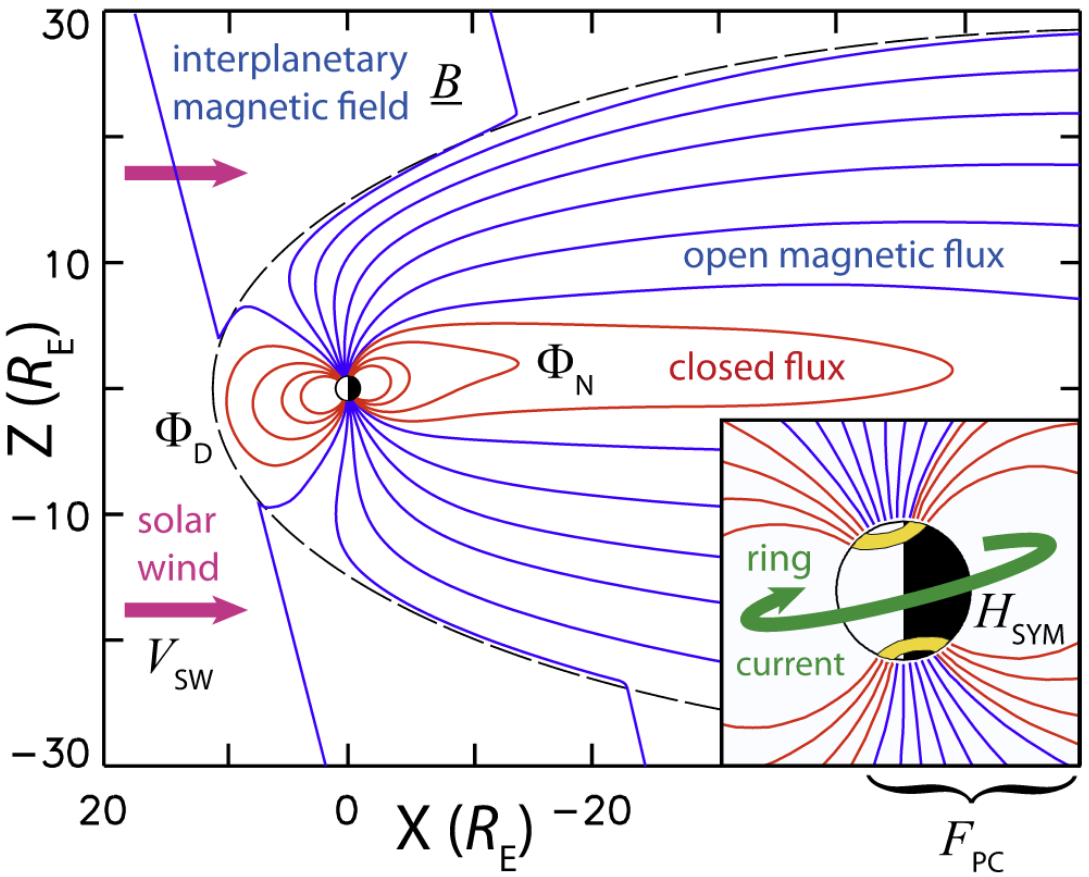
\includegraphics[width=0.6\textwidth]{figures_of_others/images/Milan2009_magnetosphere.png}
	}{
		\caption[\lofimage{figures_of_others/images/Milan2009_magnetosphere.png}]
		{Schema of the magnetosphere for the case of southern IMF direction with emphasis on open (blue lines) and closed (red lines) magnetic flux. The magnetopause is indicated by the dashed line. The opening flux rate at the dayside is denoted with $\Phi_\text{D}$ and the closing flux rate at the nightside with $\Phi_\text{N}$. The inset shows day- and nightside of Earth and the relation between auroral ovals (yellow areas) and the open flux at the polar caps ($F_\text{PC}$). The ring current intensity $H_\text{SYM}$ and direction (green arrow) are plotted as well. Credit: {\citet[Fig.~1]{Milan2009}}, \textcopyright~American Geophysical Union, reproduced with permission.}
		\label{fig:Milan2009_magnetosphere}
	}
\end{figure}
The propagation time of the solar wind from the sunward magnetopause to the magnetotail amounts to a lag of about half an hour. Thus, because the rate of reconnection scales with the changing dynamic pressure of the solar wind, the total amount of open flux $F_\text{PC}$ varies with time so that the ionospheric polar caps expand/contract with time as well \citep{Siscoe1985}:
\begin{align}
	\frac{\text{d}F_\text{PC}(t)}{\text{d}t} = \Phi_\text{D}(t) - \Phi_\text{N}(t)	\,.	\label{eq:faradays_law}
\end{align}

Continuous reconnection on the sunward magnetopause builds up the polar cap flux and thus increases stress in the magnetotail, which leads there to regular reconnection bursts, releasing the flux again.

% magnetopause reconnection
During sunward reconnection, the magnetic field component normal to the magnetopause undergoes regular bipolar oscillations that are interpreted as temporary reconnection events, transferring magnetic flux to the magnetotail. These flux transfer events occur with a period of about eight minutes \citep{Russell1996}. When solar wind conditions are steady, the reconnection process at the sunward magnetopause is found to be steady as well \citep{Phan2005}. During changing IMF direction, the reconnection site moves and intermittent reconnection has been locally observed, but the overall reconnection keeps being continuous and never ceases \citep{Phan2005}.

% tail reconnection/substorms
The reconnection in the magnetotail occurs in regular intermittent reconnection bursts. These bursts can produce magnetic plasmoids that release from the tail and are swept away with the solar wind. This pulsed reconnection has a period of a few hours and is the major nightside flux closure process \citep{Milan2007}. The subsequent effects on the magnetosphere are called substorms. Their duration varies greatly around an average value of 70~minutes and they vary in intensity as well. Substorms create sudden brightenings and increased activity in the aurora, which also show characteristic patterns matching the substorm cycle. Substorms are found to occur spontaneously during southward IMF periods, however, in \SI{60}{\percent} of the cases they are triggered by changing upstream solar wind conditions -- either by switches in the IMF orientation or by shocks in the solar wind ram pressure \citep{Milan2007}.

The arrival of extreme solar wind conditions, such as found in CMEs and CIRs, generates geomagnetic disturbances larger than substorms, these geomagnetic storms are described in \autoref{sec:geomagnetic_storms}.


\subsection{Russell-McPherron effect}
\label{sec:russell_mcpherron_effect}
Geomagnetic activity varies semiannually with the maxima around the equinoxes and the minima around solstices \citep{Cortie1912}. \citet{Russell1973} suggested a model, the Russell-McPherron (R-M) effect, that is able to predict the correct phase and the observed variation in strength seen yearly in geomagnetic activity. They define a solar wind-magnetosphere interaction in GSM coordinates that is set to zero during northward IMF and is otherwise proportional to the southward IMF component. As solar wind and IMF are naturally ordered in the geocentric solar equatorial (GSEQ) coordinate system, their flow angle against the magnetosphere undergoes seasonal changes. The mechanism then is provided by the changing probability over the year of getting a north- or southward IMF, viewed in the GSM-frame of the magnetosphere. This variation is found to be sufficient to generate the observed effect \citep{Russell1973}. An additional factor to the interaction of the R-M effect is the IMF tilt angle which is shown to regulate the extent of the sunward reconnection region and therefore the reconnection rate and geomagnetic activity \citep{Russell2003}.

There exist other hypotheses describing the semiannual variation: the axial and the equinoctial hypotheses. However, the R-M effect is the most prevailing and is even able to explain the variation of geomagnetic activity under extreme solar wind conditions, such as interplanetary shocks \citep{Zhao2012}.\\

solar-terrestrial tilt angle and orbit geometry figure? half-wave rectifier...\\


\subsection{Geomagnetic indices}
\label{sec:geomagnetic_indices}
In order to monitor the state of the magnetospheric system and disturbances therein, geomagnetic observatories are distributed widely over the globe, measuring the local magnetic field at their position. Several sets of stations, covering specific regions, are defined to monitor the state of different parts of the magnetospheric system. Magnetic measurements from these sets define a multitude of geomagnetic indices. The International Association of Geomagnetism and Aeronomy (IAGA) supports the following global geomagnetic indices which are serviced by the International Service of Geomagnetic Indices (ISGI)\footnote{ISGI website: \urlfoot{http://isgi.unistra.fr/}}:
The $aa$~index is designed to represent the amplitude of the global geomagnetic activity, normalized to a geomagnetic latitude of \SI{+-50}{\degree}. The $am$~index characterizes the global geomagnetic activity. The \Kp{}~index is designed to measure geomagnetic disturbances from solar particle radiation -- it is described in more detail in the following section. The $Dst$~index monitors the intensity of the magnetospheric ring current. The $PC$~index monitors the polar cap magnetic activity -- it approximates the amount of energy which entered the magnetosphere through solar wind coupling. The $AE$~index and its relatives $AU$, $AL$ and $AO$ measure the magnetic effects of the northern auroral electrojet.
The first three listed indices ($aa$, $am$ and \Kp{}) are calculated from different sets of local 3"~hourly $K$~indices, which measure the local magnetic disturbances at the observatories.\\
% There exist several sub-indices that are based on some of those listed above, e.g., ap, Ap, Cp, C9, Aa, Kpa, an, as, Kpm, Am, An, and As.\\


\subsection{Geomagnetic storms}
\label{sec:geomagnetic_storms}
Geomagnetic storms are major disturbances in the geomagnetic field, generated under extreme solar wind conditions. Solar wind injects plasma and energy into the magnetosphere, varying the number of particles in the magnetospheric equatorial current system that is located between \SIrange{2}{7}{\RE} \citep{Gonzalez1994}. When this ring current is increased, it generates an enhanced magnetic field of opposite polarity to the magnetospheric field. This leads to a decrease in the local terrestrial magnetic field.

% Dst index
The decrease is measured by the disturbance storm time index $Dst$, which is derived by magnetic field measurements made by four magnetic observatories located at the dipole equator \citep{Sugiura1991}. Thus, $Dst$ represents the intensity of the ring current and is a quantitative measure for geomagnetic disturbances. The $Dst$~index is derived and published through the IAGA at the World Data Center for Geomagnetism, Kyoto\footnote{WDC for Geomagnetism, Kyoto $Dst$~index service: \urlfoot{http://wdc.kugi.kyoto-u.ac.jp/dstdir/index.html}}.

Historically, the size of geomagnetic storms was defined as the peak negative disturbance in the $Dst$~index. Though, the onset of a geomagnetic storm is typically an aprupt increase in $Dst$, called storm sudden commencement (SSC). The initial positive $Dst$~values last a few hours and are caused by the compression of the magnetosphere due to the increased pressure of arriving shocked solar wind plasma. The intensity of a geomagnetic storm can be measured by the minimum $Dst$ that is reached in its main phase -- $Dst$ falls below \SI{-50}{\nano\tesla} during moderate storms and below \SI{-100}{\nano\tesla} during intense storms \citep{Gonzalez1994}. The main phase lasts a few hours, but the recovery to average $Dst$ levels is gradual and can take up to several days.\\

However, for the assessment of overall geomagnetic activity, another index has been more widely used than $Dst$, the \Kp{}~index \citep{Gonzalez1994}.\\


Furthermore, field-aligned currents connect to currents in the auroral ionosphere, the auroral electrojets, these generate large magnetic disturbances as well. Collectively with the ring current, these currents contribute to the total planetary geomagnetic disturbances. The disturbances are quantified on the ground with the planetary geomagnetic disturbance index \Kp{}.\\




NOAA/SWPC: \Kp{} is the basis for one of the three NOAA Space Weather Scales, the Geomagnetic Storm, or G-Scale, that is used to describe space weather that can disrupt systems on Earth.\\


% solar wind causes
\citet{Carrington1859} was the first to associate a geomagnetic storm with an event of solar origin, that is, he noticed a major solar flare appearing a few hours before the storm. The corresponding solar event is known as the Carrington event, as the resulting geomagnetic storm is assumed to be the largest ever observed. \citet{Forbush1937} found a rapid reduction in cosmic-ray intensity occurring parallel to a geomagnetic storm, now known as Forbush decreases, and attributed both to a common external cause. Eventually \citet{Wilson1987} demonstrated the connection between geomagnetic storms and MCs by finding simultaneous decreases in the $Dst$~index during episodes of southward IMF within MCs. The order in which north- and southward IMF appears in an MC does not matter for the final observed $Dst$ magnitude, but the $Dst$ activity is always in phase with the southward field \citep{Zhang1988}. \citet{Gosling1993} established that CMEs rather than flares are the main cause of major geomagnetic storms and large SEP events. Indeed, single and multiple CME events are found to be the most geoeffective solar wind structures in that they are accountable for about \SI{87}{\%} of the major geomagnetic storms, whereas the remainder is produced by CIR events \citep{Zhang2007}.\\


----------------\\

NOAA/SWPC:\\
Storms also result in intense currents in the magnetosphere, changes in the radiation belts, and changes in the ionosphere, including heating the ionosphere and upper atmosphere region called the thermosphere.\\


% difference to substorms
During geomagnetic storms, substorms occur in higher frequencies and can overlap each other (cite?).\\

the main phase of storms has been observed to be always accompanied by substorms \citep{Gonzalez1994}\\



\subsection{\Kp~index}
\label{sec:kp_index}

\section{Forecast methods}
\label{sec:forecast_methods}
both Newell relations\\

\subsection{Coupling functions}
\label{sec:coupling_functions}

\subsection{\Kp~forecast}
\label{sec:kp_forecast}
Kp-flux rate relation\\
Kp prediction models/methods\\
This paper adds more empirical relations.\\

\subsection{CME forecast to Earth}
CME forecast methods and models\\

\subsection{Stream forecast to Earth}
Stream forecast methods and models\\


%%%%%%%%%%%%%%%%%%%%%%%%%%%%%%%%%%%%%%%%%%%%%%%%%%%%%%%%%%

% Space weather
% 
% Magnetosphere
% Structure (currents, plasma regions)
% Solar wind coupling mechanisms (list all: reconnection, turbulence, ...)
% Dungey convection cycle (unsteady/continuous reconnection; substorms; two-cell convection)
% Russell-McPherron effect (seasonal variations)
% Geomagnetic indices
%
% Geomagnetic storms (difference to substorms; types of triggering events (CMEs, CIRs, Dst, Kp, ...)
%
% Forecast methods
% Coupling functions
% Kp forecast
% CME forecast to Earth
% Stream forecast to Earth



%%%%%%%%%%%%%%%%%%%%%%%%%%%%%%%%%%%%%%%%%%%%%%%%%%%%%%%%%%
\section{Magnetosphere}
\subsection{\Kp~index}

The MC plotted in \autoref{fig:ACE_64s_v7_thesis_CME_2013-6-26_6} created a \Kp{} of 6+.\\


\subsection{Coupling functions}

at Earth the solar wind total energy flux ($1.45~\text{mW/m}^2$) is only about one millionth of the solar radiation flux (see \citet[p.~153]{Schwenn1990})\\

reconnection behind the cusps or at the front of the magnetopause (see \autoref{fig:Bothmer1998book_p116_fig4_8_sw})\\
\begin{figure}[htb]
	\fcapside[\FBwidth]{
		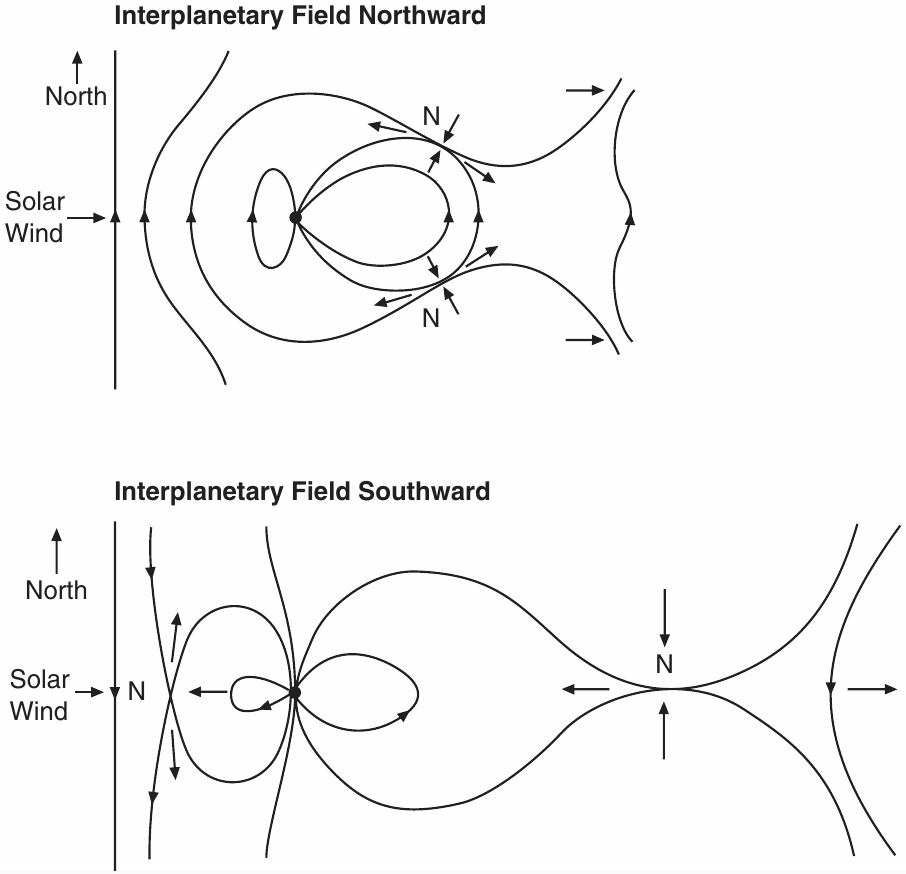
\includegraphics[width=0.6\textwidth]{figures_of_others/images/Bothmer2007book_p116_fig4_8_sw.png}
	}{
		\caption[\lofimage{figures_of_others/images/Bothmer2007book_p116_fig4_8_sw.png}]
		{Sketch indicating where reconnection of magnetic field lines on the magnetopause occurs, for the cases of northward (upper panel) and southward (lower panel) IMF. The central dot indicates the position of Earth and the arrowed lines the direction of the magnetic field. The locations of X"~line reconnection are denoted with N and the short arrows indicate the movement of the field lines. Credit: {\citet[p.~116, Fig.~4.8]{Bothmer2007}}, adapted from {\citet{Dungey1961,Dungey1963}}. get permission...}
		\label{fig:Bothmer1998book_p116_fig4_8_sw}
	}
\end{figure}

for overview see chapter~4 in Bothmer2007book\\

E-field produced by solar wind acts on magnetospheric plasma\\	%VBth p124
\begin{align}
	\textbf{E}_\text{IMF} = -\textbf{V} \times \textbf{B}_\text{IMF}
\end{align}
from Lorentz force F = -e vxB\\
E = -F/e\\
Because of high plasma conductivity the E-field is not existent.\\

% two-part solar wind coupling
\citet{Newell2007} and \citet{Newell2008}: coupling consists of merging and viscous part (reconnection and turbulence)\\
merging part: universal sw-magnetosphere coupling function; rate magnetic flux is opened at the magnetopause ($d\Phi_\text{MP}/dt$)\\
viscous part: reconnection due to Kelvin-Helmholtz instabilies at the boundary ($n^{1/2} v^2$)\\
equation for the least variance linear prediction of Kp: $Kp = 0.05 + \num{2.244e-4} d\Phi_\text{MP}/dt + \num{2.844e-6} n^{1/2} v^2$\\
combination of both terms works best (r = 0.866)\\

dayside reconnection:\\
``$E_\text{y}$ is the rate at which southward magnetic flux is convected to the magnetosphere by the solar wind ($-v_\text{x} \cdot B_\text{z}$) in GSM coordinates,'' \citep{Russell2007}\\

In this work I settle for \vBz{} as the coupling function -- that is why I focus on this relation here.\\

The solar wind electric field $E_y$ is the product of the proton velocity $v$ and the magnetic field z-component $B_\text{z}$:
\begin{align}
	E_\text{y} = -v_\text{x} \times B_\text{z}\,.	\label{eq:coupling_vxBz}
\end{align}

Savani2017:\\
...a function is required that characterizes the coupling of the solar wind to the magnetosphere. Many functions that couple the solar wind to a wide variety of magnetospheric activity have been proposed in the past, often incorporating the magnetic field orientation [Lockwood et al., 2013, and references therein]. A recent study suggests that one parameter correlates best with 9 out of 10 indices of terrestrial activity [Newell et al., 2007]. This parameter, $d\phi/dt$, represents the rate at which magnetic flux is opened at the magnetopause and is defined as\\
\begin{align}
	\frac{\text{d}\phi}{\text{d}t} = v^{4/3} |B|^{2/3} \sin^{8/3}(\theta_c/2)
\end{align}
where v is the velocity of the solar wind; |B| is the magnetic field magnitude; and the interplanetary magnetic field (IMF) clock angle is defined by $\theta_c = \tan^{-1}(By/Bz)$. The predicted magnetic field time series in GSM coordinate system is used to calculate a theoretical magnetic flux rate.\\


% Bz importance for geomagnetic storms
connection between geomagnetic disturbances and the southward component of the external interplanetary magnetic field (\citep{Dungey1961}; Fairfield and Cahill Jr 1966).\\


\section{Forecast methods}
"The principal users affected by geomagnetic storms are the electrical power grid, spacecraft operations, users of radio signals that reflect off of or pass through the ionosphere, and observers of the aurora." NOAA cite\\


Methods:\\
- MC Kp impact forecast; Savani2015+Savani2017\\
- WSA-ENLIL sw forecast (CMEs without B-field)\\
- CH sw forecast (Uni Graz)\\
- NOAA/SWPC; see Savani2017\\
- NASA/SWRC; see Savani2017\\

\subsection{\Kp~forecast} (quantitative)

Space weather effects can be directly attributed to CME sub-structures. While the outermost structure (shock) accelerates particles and causes sudden commencement, the interior structures (sheath and flux rope) cause geomagnetic storms if they possess a strong southward component of the magnetic field \citep{Gopalswamy2016}.\\

see Wing Kp model description...\\
%https://www.swpc.noaa.gov/products/wing-kp

% Bz prediction
Southward interplanetary field can also occur in the shock sheaths (Gonzalez and Tsurutani 1987; Gosling and McComas 1987), which have been shown to be equally important in causing geomagnetic storms \citep{Tsurutani1988}.\\
The results of this study indicate the equal importance of both sheath fields or draped fields and driver gas fields for the generation of major geomagnetic storms. Because of the importance of the sheath fields the intensity and duration of geomagnetic storms cannot be predicted by solar observations of active regions alone \citep{Tsurutani1988}.\\

read Savani2015: Predicting the magnetic vectors within coronal mass ejections arriving at Earth: 2. Geomagnetic response\\

It makes sense to use the geocentric solar magnetospheric (GSM) coordinate system, which is aligned with the Earth's magnetic dipole axis.\\

Savani2015:\\
The compressed solar wind plasma in between supersonic magnetic flux rope obstacles and their driven shock fronts has not been addressed in this article, even though they have been shown to be significant drivers of magnetospheric storms [Huttunen and Koskinen, 2004].\\

Savani2017:\\
The correlation coefficient of $d\phi/dt$ with the \Kp~index is $r = 0.76$ [see Newell et al., 2007, Table 3]. A Kp prediction is then generated by the empirical correlation.\\
\begin{align}
	\Kp(BSS) = 9.5 - e^{A-B(d\phi/dt)}
\end{align}
where $A = 2.18, B = 5.20 * 10^5$ , and with the velocity and magnetic field measured in km/s and nT, respectively [Emmons et al., 2013; Mays et al., 2015a].\\


\subsection{CME forecast}

Predicting the magnetic field variations in ICMEs from solar observations is a central subject for space weather forecasting because a long-lasting southward-directed  field is a primary driver of major geomagnetic storms \citep{Zhang2007}.\\

Identification of a flux rope near the Sun makes it easier to predict the expected magnetic configuration at Earth, modified by the interaction with the solar wind on its way to Earth.\\

Bz prediction:\\
read Savani2015: Predicting the magnetic vectors within coronal mass ejections arriving at Earth: 1. Initial architecture\\

Savani2015:\\
Thus, models used for routine CME forecasts by various space weather services do not include magnetic structures within the simulated CMEs [e.g., Zheng et al., 2013; Shiota et al., 2014]. For example, ENLIL models the propagation of CMEs from ~20 solar radii (Rs ) to beyond Earth at 215 Rs and includes the background solar wind magnetic field. However, the CME is simplified to a high-pressure plasma pulse with a size and propagation direction estimated from solar imagery [Zheng et al., 2013]. CME arrival time predictions from these models provide lead times of ~2–3 days, and their accuracy has been well investigated [Taktakishvili et al., 2010; Vršnak et al., 2014; Colaninno et al., 2013]. In contrast, the important magnetic vector information is only revealed when in situ measurements are made by spacecraft upstream of Earth at the first Lagrangian position (L1) ~1 h prior to the CME arriving at Earth, thereby severely limiting the lead time available for reliable, magnetic field-based, storm warnings.\\
Savani2015:\\
In this paper, we highlight three key components of a proof of concept developed to improve the prediction of a storm’s severity: (1) the use of the hemispheric helicity rule to provide a robust initial magnetic configuration at the Sun; (2) define a “volume of influence” of the CME, within the heliosphere, for which the Earth’s trajectory can be estimated; and (3) incorporating magnetic vectors from a simplified magnetic flux rope model to create a time series upstream of Earth.\\


constant-alpha force-free (CAFF) flux ropes (Burlaga1988)\\

adjusted BSS scheme (Savani2015)\\

Savani2017:\\
inferring the magnetic field direction along the trajectory of Earth through the CME would be a major advance in geomagnetic activity prediction.\\

Savani2017:\\
This event highlights the need to forecast the field vectors not only in the flux rope but also in the sheath [e.g., Huttunen and Koskinen, 2004].\\


% CME forecast
It is important to know in advance if and when CMEs arrive at Earth, because of their possible strong impact on the terrestrial magnetosphere. Knowing the geometry of a CME, it is possible to infer its direction and speed from white-light images. Through kinematic forward-modeling techniques that take advantage of the self-similar expansion observed in CMEs, it is possible to derive an estimated arrival time at Earth. As MCs are the drivers for most severe geomagnetic disturbances \citep{Bothmer1995,Cane2003}, it is also important to forecast their magnetic field strength and configuration.

% 3D models
An early 3D model for a general CME geometry is the ice-cream cone model, which assumes a simple bubble-like CME structure \citep{Fisher1984}. Though, building on the the study by \citet{Cremades2004}, \citet{Thernisien2006} created the more complex graduated cylindrical shell (GCS) model for flux rope-like CMEs. This model assumes an empirically derived electron distribution in order to create synthetic coronagraph images. The GCS model is successfully applied to images of CMEs with well-developed white-light structure \citep{Bosman2012} and is implemented as a part of current CME forecast procedures.\\



% CME kinematics
Depending on wether CMEs are faster or slower than the surrounding solar wind, they decelerate/accelerate on their way through the heliosphere due to the drag forces. Fast CMEs already decelerate substantially during their first few solar radii \citep{Sachdeva2017}. In case a CME interacts with a preceding CME, they both travel on with an intermediate speed \citep{Manoharan2004,Temmer2012}.

% extreme events
Extreme CME velocities above \SI{2000}{\km\per\s} near the Sun are rare, nevertheless, in some cases speeds around \SI{3000}{\km\per\s} were measured. From the free energy available in active regions, \citet{Gopalswamy2005} concluded that CME speeds cannot be far greater than \SI{3000}{\km\per\s}. This would implicate that CMEs need at least half a day to travel from their source region on the Sun to reach Earth. \citet{Gopalswamy2010} even estimated a maximal limit of free energy active regions can store, which means that CMEs with \SI{4000}{\km\per\s} are not possible. Faster CMEs usually come with higher magnetic field strengths, for example the CME observed by STEREO~A on 23~July 2012 had a shock speed of about \SI{2000}{\km\per\s} at \SI{1}{\au} and its magnetic field magnitude reached values of up to \SI{100}{\nT} \citep{Russell2013}.\\


% halo CMEs:
observed coronal transient: 3d structure, directed at Earth, associated with shock wave; \citep{Howard1982} -> halo CME\\


\subsection{Stream forecast}

Cranmer2017:\\
Complicating our understanding even more is the fact that processes such as turbulence, stream-stream interactions, and Coulomb collisions can make it difficult to unambiguously map a parcel measured at 1 AU back down to its coronal source.\\


\section{notes...}

These events (GS) are able to disturb sensitive technical systems. Understanding the properties of the solar wind helps with the prediction and protection of humanity's assets.\\

reference to \citet{Bothmer2007}, maybe images\\

put fig. somewhere earlier (p.~10?): see \autoref{fig:Hundhausen1977_fig20bcd}\\
\begin{figure}[htb]
	\centering
	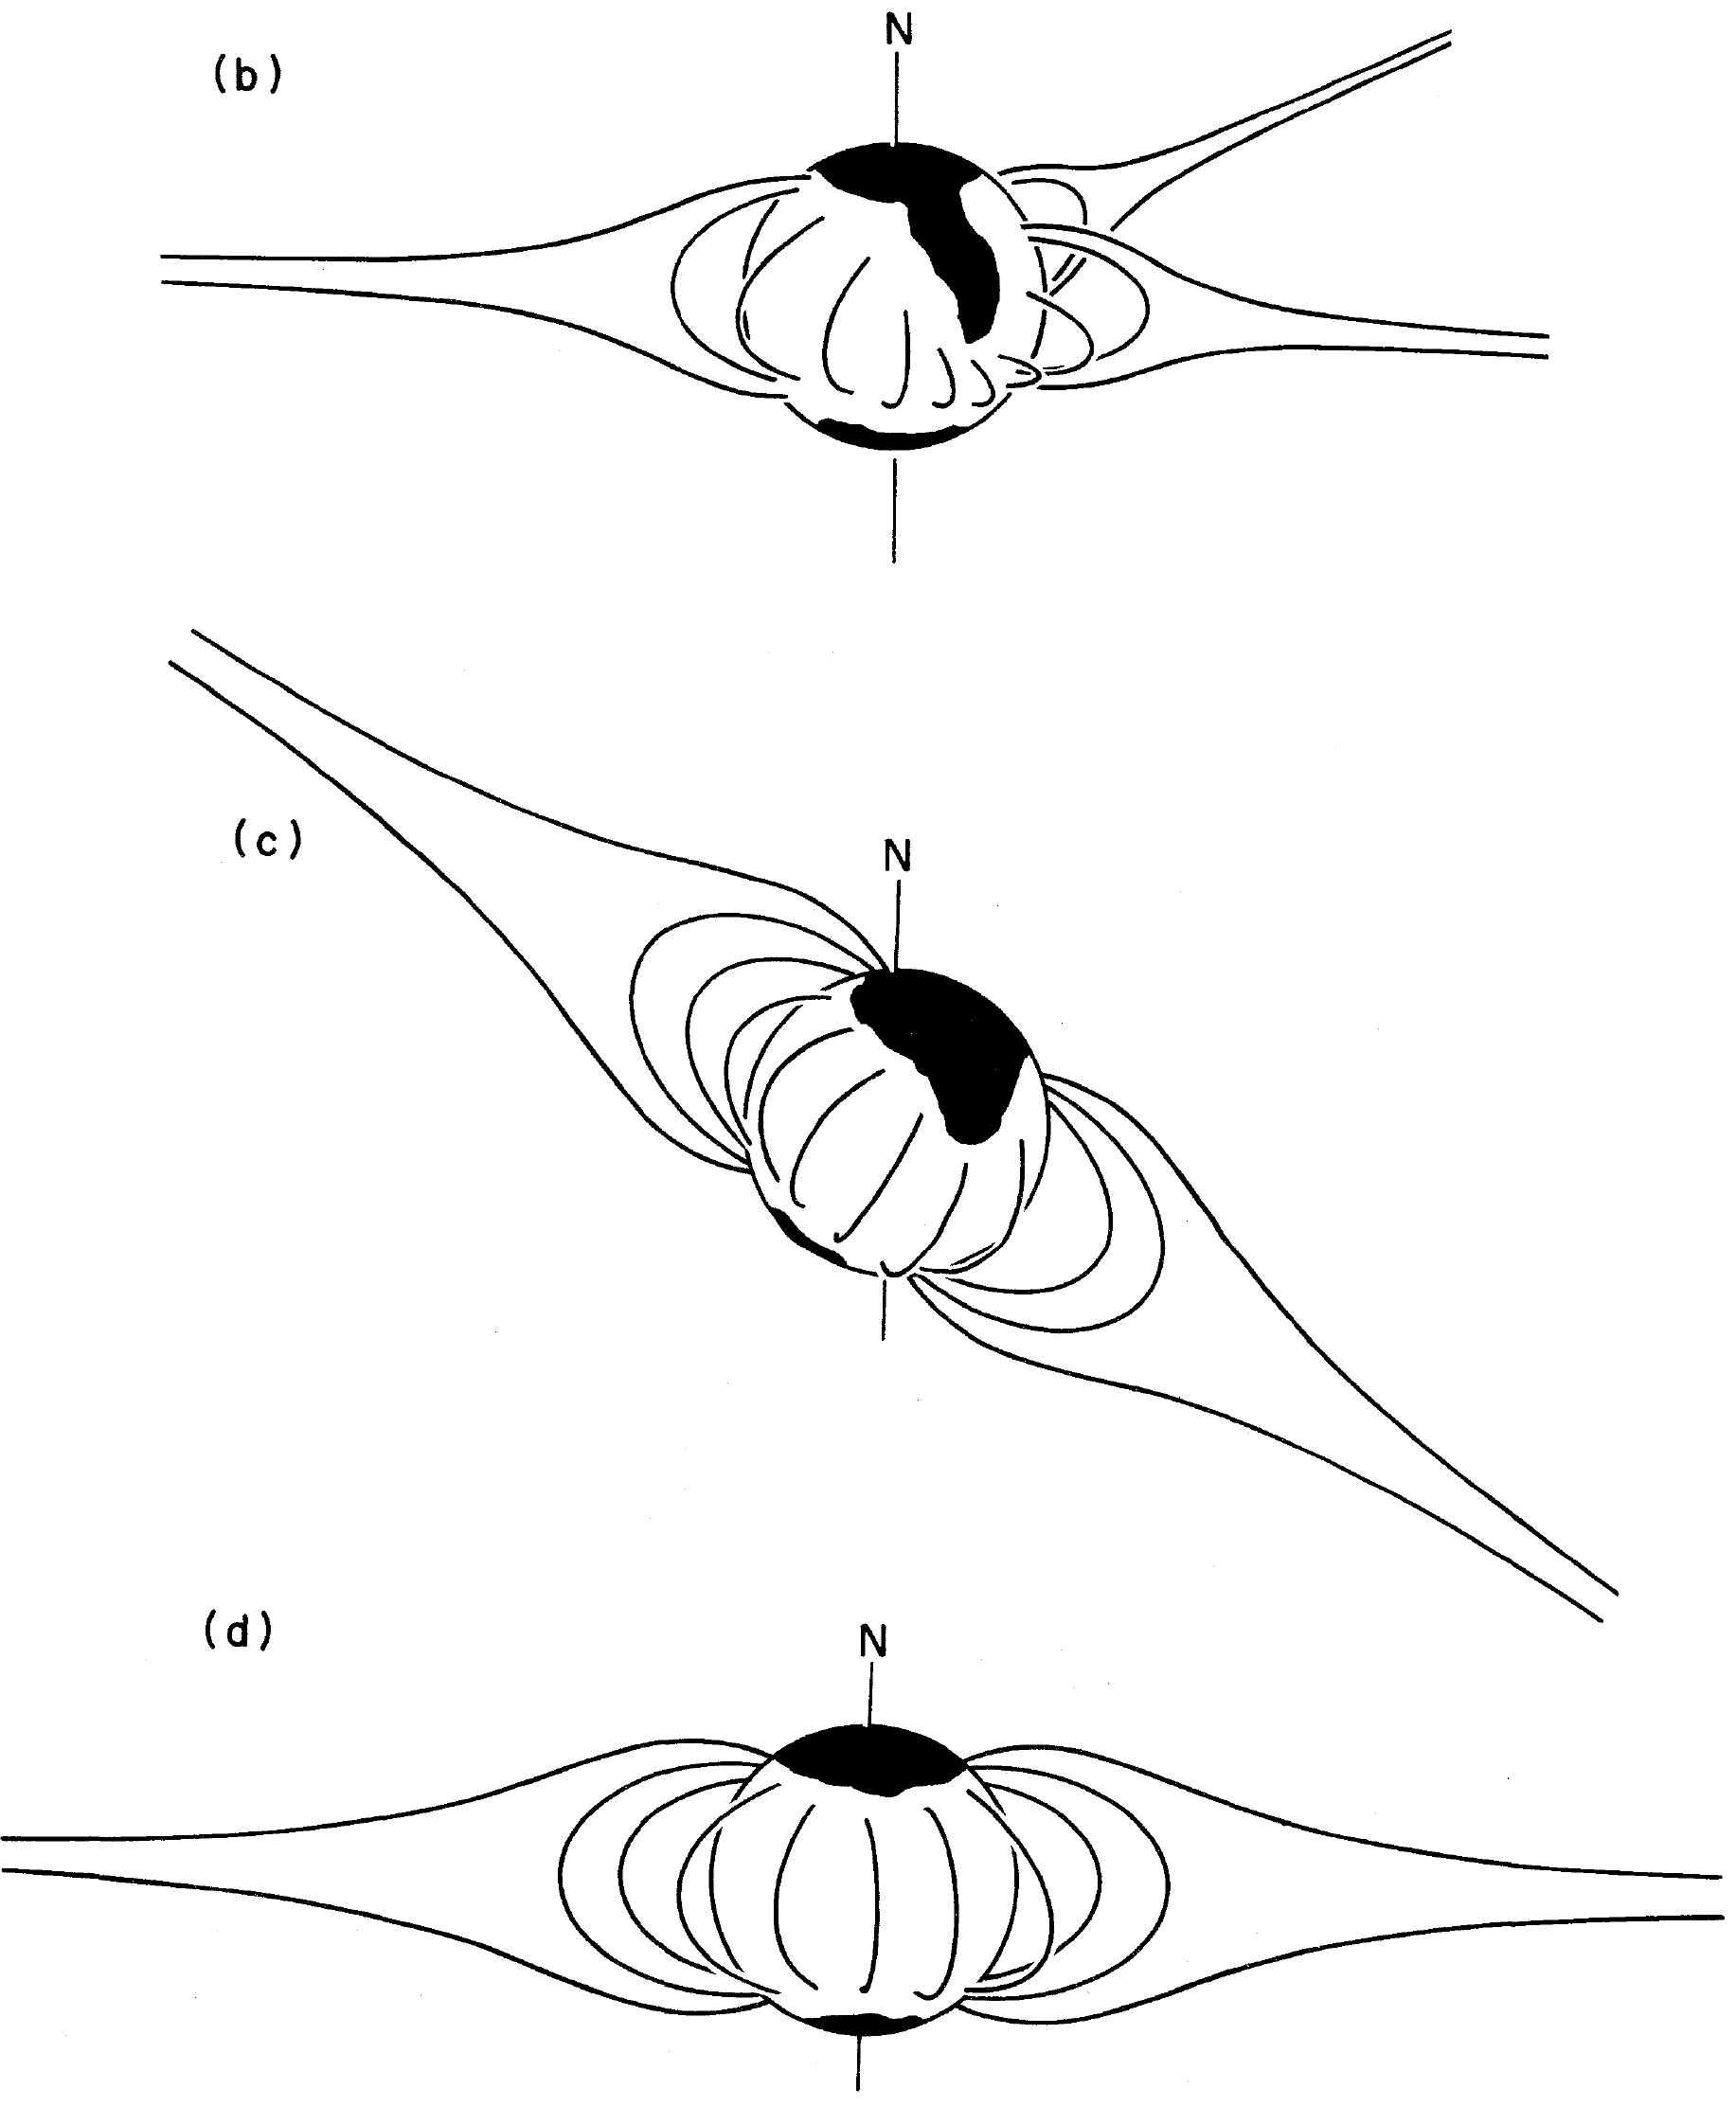
\includegraphics[width=0.5\textwidth]{figures_of_others/images/Hundhausen1977_fig20bcd.png}
	\caption[\lofimage{figures_of_others/images/Hundhausen1977_fig20bcd.png}Credit: {\citep[Fig.~20, panels (b--d)]{Hundhausen1977}}, \textcopyright~Colorado Associated University Press, reproduced with permission.]
	{Schemata of different coronal configurations during the solar cycle. Visualized are the locations of closed coronal magnetic fields (lines) and coronal holes (black areas) for a post maximum distorted dipole (top panel), for a pre minimum stable tilted dipole (middle panel), and a post minimum axial dipole (bottom panel). Credit: {\citep[Fig.~20, panels (b--d)]{Hundhausen1977}}, \textcopyright~Colorado Associated University Press, reproduced with permission.}
	\label{fig:Hundhausen1977_fig20bcd}
\end{figure}


% low solar activity influence on geomagnetic storms/space weather
The weaker solar activity cycle 24 seems to have important consequences for CMEs in the heliosphere: CMEs expand anomalously due to reduced heliospheric pressure leading to the increased observed rate of small CMEs, halos originating far from the disk center, and mild space weather (\citep{Gopalswamy2014}, 2015a; Petrie 2015).\\
The total pressure in the heliosphere (magnetic + plasma) is reduced by ca. 40\%, which leads to the anomalous expansion of CMEs explaining the increased slope. The excess CME expansion contributes to the diminished effectiveness of CMEs in producing magnetic storms during cycle 24, both because the magnetic content of the CMEs is diluted and also because of the weaker ambient fields \citep{Gopalswamy2014}.\\

the dayside reconnection is asymmetric\\
half-wave rectifier coupling\\
To describe this, coupling functions with different complexity were proposed (Newell, cites? and list).\\
Newell's relation is being implemented into forecast procedures (Savani2017)\\

causes (see citet{Rangarajan1997} p.~1282 and mention Bartels1963 too)\\
read Bothmer1998 Ch 3...\\


\citet{Sonnerup1967}: The rotational discontinuity seems to occur predominantly during magnetic storms and two of these cases, involving substantial normal-field components, provide compelling evidence that field reconnection takes place during the storm main phase.\\

read Milan2009\\	% http://adsabs.harvard.edu/abs/2009GeoRL..3618101M

% mass flux considerations:\\
% mass per second per Earth disc...\\
% R_E = 6371.008 km\\
% A_E = pi * R_E² = 127516438.219 km²\\
% m_p = 1.672621898e-27 kg\\
% v = 400 km/s\\
% n = 6.5 cm-3 = 6.5e15 km-3\\
% mass flux = m_p * n * v * A_E = 0.0013863641126 kg/s/A_E\\
% = 1.4 g/s/A_E = 5 kg/h = 120 kg/d/A_E = 44 t/a/A_E\\

% Wikipedia: https://en.wikipedia.org/wiki/Solar_wind
% The wind exerts a pressure at 1 AU typically in the range of 1–6 nPa (1–6×10−9 N/m2), although it can readily vary outside that range.
% The ram pressure is a function of wind speed and density. The formula is
% P = mp * n * V2= 1.6726×10−6 * n * V2
% where mp is the proton mass, pressure P is in nPa (nanopascals), n is the density in particles/cm3 and V is the speed in km/s of the solar wind.[citation needed]


sources of southward Bz:\\
- MCs\\
- compressed material in front of CMEs (highest driving velocities)\\
- SIRs/CIRs front of HSSs\\
- sw streams\\


% CMEs
3-part structure figure ... find event with shock and flux rope?\\
abbreviate magnetic flux rope to MFR?\\
 
% HCS
why HCS? what currents are there...\\
why is the CS not the divide between both polarities?\\

% space weather
strong radio bursts...\\

% magnetosphere
ring current systems\\

radiation belts\\

Phan2005, Magnetopause Processes:\\
Cluster findings include:\\
A strong ‘guide field’ detected at a reconnection X-line, i.e., a finite magnetic field along the X-line, has provided direct evidence for component merging.\\
Tailward-of-the-cusp reconnection has been found to occur only when the IMF has a northward component. The occurrence rate of cusp reconnection is nearly 100\% when the IMF has a northward component, implying that cusp reconnection in the northern and southern hemispheres must be common. The high occurrence rate (in contrast to a rate of 50\% at the subsolar magnetopause) is thought to be due to the presence of a plasma depletion layer. In this layer, the plasma beta is reduced, rendering the magnetosheath flow sub-Alfvenic and allowing the establishment of a stable X-line at the high-latitude magnetopause.\\

look into printed paper collection...\\

% geomagnetic indices
\citet{Lockwood2014} even used geomagnetic indices (including $aa$) to reconstruct the near-Earth IMF strength and solar wind flow speed back to 1845.\\




%%%%--  next chapter  --%%%%

\chapter{Instrumentation and data description}
\label{chap:data}
%COFI -- chapter outline and flow integration
For analyzing the solar wind and related areas on the Sun, there exist remote instruments, such as solar imagers and coronagraphs, and in-situ instruments, such as magnetometers and plasma detectors. In this chapter the basic principles of the latter are described, because the analyses performed in this thesis are based entirely on in-situ measurements -- except for the sunspot time series.

Different kind of data, collected from observatories at various locations, are used for the investigations performed in this thesis. In the following sections, I describe the data sets of the magnetospheric disturbance index \Kp{} and of the solar activity indicator sunspot number (SSN). Further, the solar wind in-situ data sets are described: the near-Earth OMNI data collections consisting of minutely and hourly data, that is, low resolution OMNI (LRO) and high resolution OMNI (HRO), and the data obtained from the Helios~1 and Helios~2 spacecraft in the 1970s. I plotted a time coverage overview of these data sets in relation to the solar activity cycles in \autoref{fig:timeline_SSN_with_data_and_sc}.\\
\begin{figure}[htb]
	\centering
	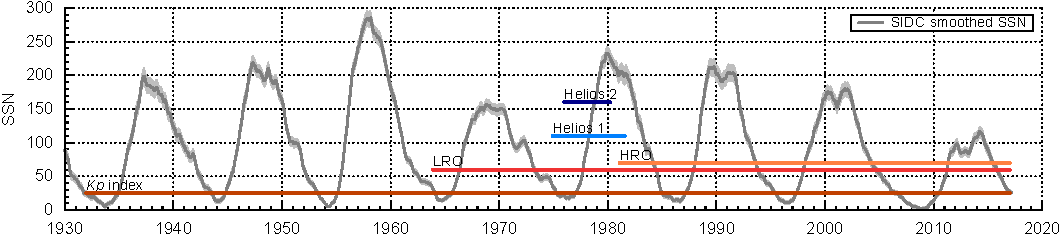
\includegraphics[width=\textwidth]{figures_of_mine/gnuplots/timeline_SSN_with_data_and_sc.pdf}
	\caption[\lofimage{figures_of_mine/gnuplots/timeline_SSN_with_data_and_sc.pdf}]
	{Time coverage of the data sets used in this work with the solar activity from 1930 until end of 2016. The individual data sets are the \Kp~index, the low and high resolution OMNI (LRO and HRO) collections, and the Helios~1 and Helios~2 data sets. I plotted the SIDC 13-month smoothed monthly SSN and the cycle number in the background for orientation.}
	\label{fig:timeline_SSN_with_data_and_sc}
	\addtocontents{lof}{\smallskip\protect\center I created the figure myself.\medskip}
\end{figure}
% 
% Spacecraft / data sets\\
% Positions:\\
% Earth:\\
% 	imager, magnetosphere\\
% L1 - first Lagrangian point:\\
% 	ACE (siehe auch space weather spacecraft Liste)\\
% 	Wind etc. (OMNI)\\
% 	DSCOVR\\
% 1~au orbit\\
% 	STEREO~A and B\\
% inner heliosphere:\\
% 	Helios~1 and 2\\
% 	PSP\\
% outer heliosphere:\\
% 	Voyager~1 and 2\\
% 	Ulysses\\


\section{Magnetometer}
%\label{sec:magnetometer}

Spacecraft nowadays carry two different magnetometer types, one for measuring the magnetic field direction and its strength and the other for observing the magnetic flux and detecting waves.\\

A flux-gate magnetometer consists of two coils around a core -- one coil with alternating current, wich is compared with the induced current signal from the other. Without external magnetic field both patterns match. The core is easier magnetized in direction of an existing external magnetic field, in which case the patterns differ. It measures...\\
In a search coil magnetometer one coil is placed around a core; measures plasma waves -- where?\\

Because these magnetometer types are directional, they often are placed in two sets of triaxial configurations, attached on booms to minimize the influence of the spacecraft's own magnetic field.\\
L-> which is generated by surface charges?/electrons?/ionization?/the instruments?\\
%https://en.wikipedia.org/wiki/Spacecraft_magnetometer

figures and references...!\\

Ground based magnetometers measure the local magnetic field of the Earth. They already exist since...\\

examples:\\
ACE/MAG -- flux-gate magnetometer\\

%https://en.wikipedia.org/wiki/Spacecraft_magnetometer


\section{Plasma detector}
%\label{sec:plasma_detector}

several spectrometers with different energy ranges\\

isotope spectrometer - isotopic abundances of SEPs\\
ionic charge analyzer - charge state of SEPs\\
solar wind ion mass spectrometer - \\
solar wind ion composition spectrometer - \\
radio burst tracker\\


A plasma detector measures the ion energy frequency distribution, which consists basically only of protons and alphas in solar wind. I prepared a synthetic ion energy spectrum for illustration in \autoref{fig:ion_energy_spectrum_plot}.\\
\begin{figure}[htb]
	\fcapside[\FBwidth]{
		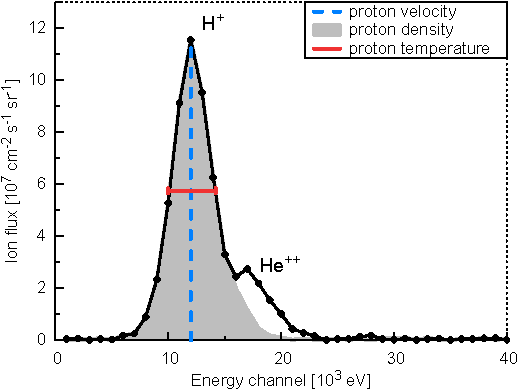
\includegraphics[width=0.6\textwidth]{figures_of_mine/gnuplots/ion_energy_spectrum_plot.pdf}
	}{
		\caption[\lofimage{figures_of_mine/gnuplots/ion_energy_spectrum_plot.pdf}]
		{Example of an ion energy spectrum for which I prepared some synthetic data points, including a small helium peak. capitalize Proton...}
		\label{fig:ion_energy_spectrum_plot}
	}
	\addtocontents{lof}{\smallskip\protect\center I created the figure myself.\medskip}
\end{figure}
%figure adapted from source: http://www.goembel.biz/sun.html
...read \url{http://www.goembel.biz/sun.html}\\

The velocity, density, and temperature can be derived from the energy spectrum.\\
more details...!\\

The bulk velocity is derived from the distribution's average energy (or position of Maxwell-Boltzmann distribution?).\\
The number density is the area of the distribution.\\
The temperature scales with the distribution's width.\\

% source: ftp://spdf.gsfc.nasa.gov/pub/data/ulysses/plasma/swoops/ion/swoops_ion_users_guide_update_20030214.txt
% ``Plasma parameters are calculated by numerical integration of velocity-weighted
% ion distributions over a E/q range chosen to include the thermal proton and
% alpha-particle populations. Under extremely hot conditions, there can
% sometimes be some overlap between these populations. Additionally, during
% periods when the solar wind temperature is exceptionally low the experiment can
% not properly measure the temperature. Care has been taken to estimate the
% instrument background from channels that do not contain data, and the effects
% of background have been removed from the integration. The velocity space 
% resolution of the experiment is better in the energy dimension than in the
% angular dimensions.''

ACE/SWEPAM\\	%https://sci-hub.ac/10.1023/A:1005040232597


\section{\Kp{}~data}
\label{sec:kp_data}
Julius~Bartels introduced the \textit{K}~index in 1938 and designed it to measure the intensity of geomagnetic disturbances \citep{Bartels1939}. Its name originates from 'Kennziffer' -- the german word for characteristic digit. The \textit{K}~index is a measure for the maximal variation of the surface magnetic field, observed in a magnetogram within 3"~hour intervals. Its scale in the range 0--9 is a quasi-logarithmic representation of the actual magnetic field strength's variations.

The Planetary \textit{K}~index (\Kp{}) is a planetary geomagnetic disturbance index, introduced by Bartels in 1949 at the Institute for Geophysics, University of Göttingen \citep{Bartels1949}. \Kp{} is the weighted average of 13 \textit{Ks}~indices, which are the standardized versions of the local \textit{K} indices measured at 13 observatories. These contributing observatories are located around \SI{+-50}{\degree} geomagnetic latitude and their distribution is biased towards Europe, see the map in \autoref{fig:Kp_map}.
\begin{figure}[htb]
	\fcapside[\FBwidth]{
		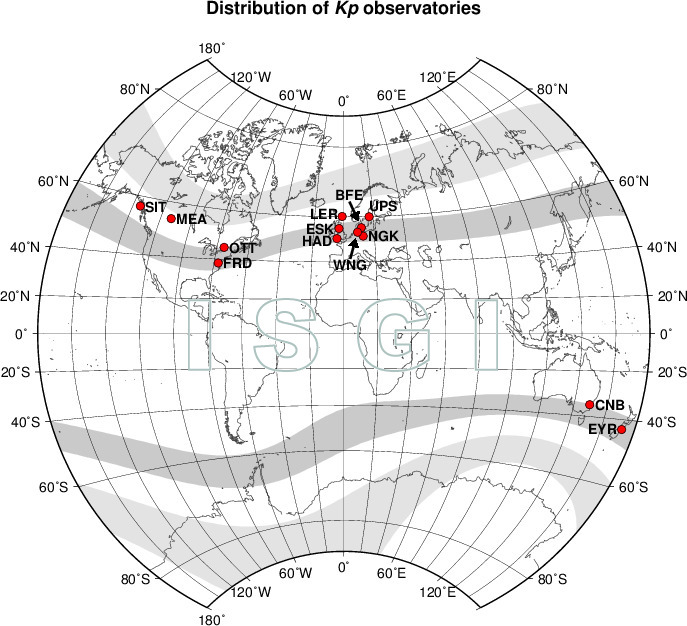
\includegraphics[width=0.6\textwidth]{figures_of_others/images/Kp_map.jpg}
	}{
		\caption[\lofimage{figures_of_others/images/Kp_map.jpg}Courtesy of \href{http://isgi.unistra.fr/indices_kp.php}{International Service of Geomagnetic Indices (ISGI)}, 2013.]
		{Distribution of the 13 \Kp{} observatories. The shaded belts indicate regions of equal geomagnetic latitude. Courtesy of \href{http://isgi.unistra.fr/indices_kp.php}{International Service of Geomagnetic Indices (ISGI)}, 2013.}
		\label{fig:Kp_map}
	}
\end{figure}
% contacted via email: got permission
%\urlfoot{http://isgi.unistra.fr/indices_kp.php}

To benefit from its higher precision, its scale, in the range 0--9 as well, is further divided into thirds, represented by the suffixes '$+$', 'o' and '$-$' (e.g., 3o, $3+$, $4-$, 4o). The \Kp{}~indices are often visualized in musical diagrams, where they are stacked into periods of 27~days to enable the detection of recurrent activities, as seen in \autoref{fig:musi1612}.
\begin{figure}[htb]
	\centering
	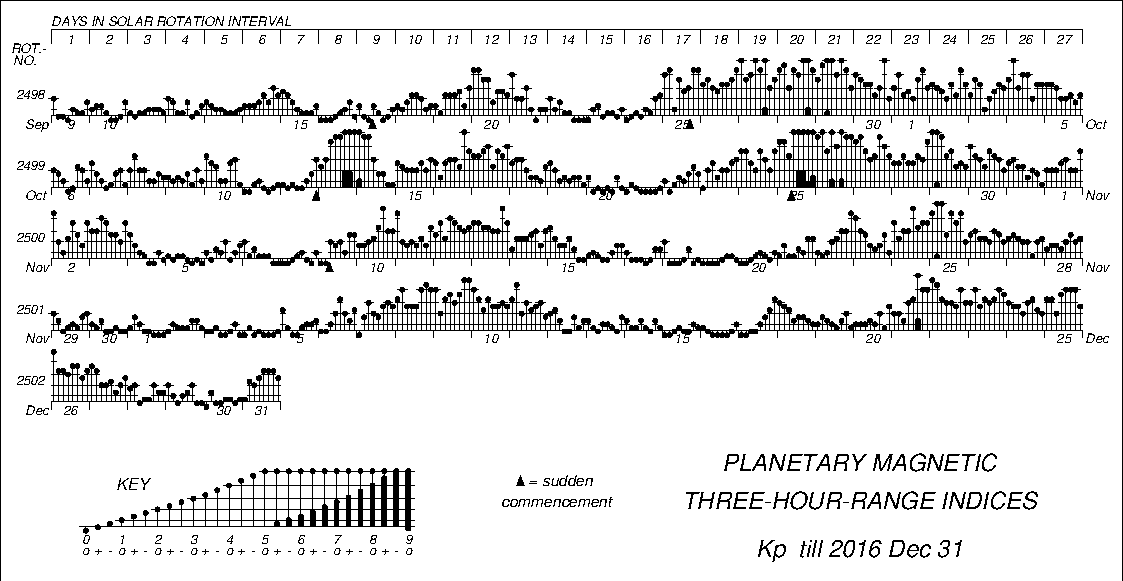
\includegraphics[width=\textwidth]{figures_of_others/images/musi1612.pdf}
	\caption[\lofimage{figures_of_others/images/musi1612.pdf}Credit: \href{http://www.gfz-potsdam.de/en/kp-index/}{GFZ~Potsdam}, 2017, licensed under \href{https://creativecommons.org/licenses/by/4.0/}{CC BY 4.0}.]
	{Bartels musical \Kp{} diagram for the time period from September until end of December 2016. Two sudden commencements with following geomagnetic storms, having a maximal \Kp{} of $6+$, can be seen in October. Credit: \href{http://www.gfz-potsdam.de/en/kp-index/}{GFZ~Potsdam}, 2017, licensed under \href{https://creativecommons.org/licenses/by/4.0/}{CC BY 4.0}.}
	\label{fig:musi1612}
\end{figure}
%ftp://ftp.gfz-potsdam.de/pub/home/obs/kp-ap/music/

The \Kp{}~index can be converted to the 3"~hour equivalent $ap$~index, which represents the magnetic field strength at a surface position of about \SI{50}{\degree} dipole latitude. The conversion is done via a table specified by Bartels, in which the value of the \textit{ap}~index is scaled in units of \SI{2}{nT}, as seen in \autoref{tab:kp_to_ap_table}.
\begin{table}
	\caption{Table for the fixed conversion from the \Kp~index to the equivalent \textit{ap}~index, which represents the magnetic field strength in units of \SI{2}{nT}.}
	\label{tab:kp_to_ap_table}
	\centering
	\begin{tabular}{lssssssssssssss}
		\Kp	&0o	&0+	&1-	&1o	&1+	&2-	&2o	&2+	&3-	&3o	&3+	&4-	&4o	&4+\\
		\textit{ap}	&0	&2	&3	&4	&5	&6	&7	&9	&12	&15	&18	&22	&27	&32\\
		\hline
		\Kp	&5-	&5o	&5+	&6-	&6o	&6+	&7-	&7o	&7+	&8-	&8o	&8+	&9-	&9o\\
		\textit{ap}	&39	&48	&56	&67	&80	&94	&111	&132	&154	&179	&207	&236	&300	&400
	\end{tabular}
\end{table}
There are further geomagnetic indices which are derived from the \Kp{}~index. They include $Ap$, the daily $ap$ average, $Cp$, the daily $ap$ sum mapped via a fixed table to the range \numrange{0}{2.5}, and $C9$, a mapping of $Cp$ via a fixed table to the range \numrange{0}{9}. The definitions of Q"~days (quiet days) and D"~days (disturbed days) are also obtained from the \Kp{}~index.

The International Association of Geomagnetism and Aeronomy (IAGA) adopted the \Kp{}~index in 1954. The \Kp{}~index was maintained in Göttingen until January 1997 -- now the German Research Centre for Geosciences (GFZ) in Potsdam supplies the \Kp{}~index and thereof derived indices. The GFZ provides historical and quicklook data of the indices via their website\footnote{GFZ website for geomagnetic indices: \urlfoot{http://www.gfz-potsdam.de/en/kp-index/}}. The data series was extended backwards using existing measurements and is now available from 1932 onwards.\\

There exist several indicators/quantities that scale or are based on the \Kp{}~index:
\begin{itemize*}
	\item NOAA's Space Weather Prediction Center (SWPC) developed its NOAA~G-Scale\footnote{NOAA Space Weather Scales website: \urlfoot{http://www.swpc.noaa.gov/noaa-scales-explanation}} for geomagnetic storms which relates the \Kp~index to five levels from G\,1 to G\,5.
	\item The equatorward auroral boundary position correlates with the \Kp~index (cite?).
	\item The variation of the total electron content (TEC) of the ionosphere correlates with the \Kp~index (cite?). The TEC has influence on global navigation satellite systems (GNSS). A part of their positional error scales directly with TEC (in extreme cases up to about \SI{30}{\m}).
\end{itemize*}


'The \Kp{}~index is designed to measure solar particle radiation by its magnetic effects.'\\

Because of the geomagnetic disturbance impacts on sensitive technical systems, various methods for now- and forecasting the \Kp{} index are developed:
\begin{itemize*}
	\item GFZ~Potsdam Nowcast \Kp~index\footnote{GFZ~Potsdam Nowcast \Kp~index website: \urlfoot{http://www-app3.gfz-potsdam.de/kp_index/ql_bar.gif}}.
	\item USAF Wing \Kp{} model \citep{Wing2005}; 1--4~hours foercast from real-time solar wind measurements\footnote{USAF Wing \Kp~model website: \urlfoot{https://www.swpc.noaa.gov/products/wing-kp}}
	\item ?Alexej \Kp{} correlation forecast model; developed within AFFECTS (link)
	\item In \autoref{chap:chapter2} of this work, I derive relations to enable \Kp{} nowcast from in-situ solar wind measurements and to enable \Kp{} forecast from remote CME/solar wind stream observations.
\end{itemize*}


Savani2017:\\
Kp is the global magnetospheric index often used by forecasters to indicate the severity of a space weather event \citep{Wing2005}.\\

Savani2017:\\
The Kp difference of 1.5 is tested as there is evidence that a limitation in accuracy is present in the underlying empirical Kp formulation [Mays et al., 2015a]. [...] which is approximately consistent with recent results by Mays et al. [2015a], the Kp empirical formulation is accurate to about Kp = 1.5.\\


see also \ref{sec:kp_index}\\

% acknowledgments:\\
% The results presented in this thesis rely on the \Kp{}~index, calculated and made available by the German Research Centre for Geosciences in Potsdam from data collected at magnetic observatories. We thank the involved national institutes, the INTERMAGNET network and ISGI (isgi.unistra.fr).\\


\section{Sunspot number}
\label{sec:sunspot_number}
The number of sunspots occuring on the solar surface is commonly used as a long-term solar activity indicator, for more information on solar activity and sunspots see \autoref{sec:solar_activity_cycle}. The international sunspot number (SSN) is maintained by the World Data Center -- Sunspot Index and Long-term Solar Observations (WDC-SILSO) at the Solar Influences Data Center (SIDC), Royal Observatory of Belgium (ROB). The SIDC provides an online catalogue\footnote{WDC-SILSO website: \urlfoot{http://www.sidc.be/silso/}}, where I obtained the SSN data. The SSN version~2.0, the current recalibrated version introduced in July 2015, is used in this work. \autoref{chap:chapter2} uses the SSN data from the time period 1932--2016, see \autoref{fig:timeline_SSN_with_data_and_sc}.

Short-term predictions of the SSN are provided by several institutions. The SIDC itself provides 12-month SSN forecasts derived via different methods. The Space Weather Prediction Center (SWPC) at the National Oceanic and Atmospheric Administration (NOAA) supports the SSN prediction of the Solar Cycle~24 Prediction Panel\footnote{Solar Cycle~24 Prediction Panel website: \urlfoot{http://www.swpc.noaa.gov/products/solar-cycle-progression}}.


\section{OMNI data collection}
\label{sec:omni_data_collection}
Solar wind was measured in~situ for the first time by spacecraft in 1959 and since 1963 near-Earth measurements were done almost continuously. The OMNI~2 data collection \citep{King2005} merges data from solar wind magnetic field and plasma, energetic proton fluxes, geomagnetic indices, and solar indices. The included solar wind data starts in \mbox{1963-11-27}, the temperature data not before \mbox{1965-07-26}, and is continuously maintained until today. As the data covers decades from multiple spacecraft at varying locations, the solar wind data is composed of intercalibrated data, which has been time-shifted to the nose of the magnetosphere's bow shock upstream of Earth. I created an overview of the various spacecraft contributing to the IMF and solar wind plasma data and their time coverages to the data set in \autoref{fig:timeline_OMNI_SC_IDs}.
\begin{figure}[htb]
	\centering
	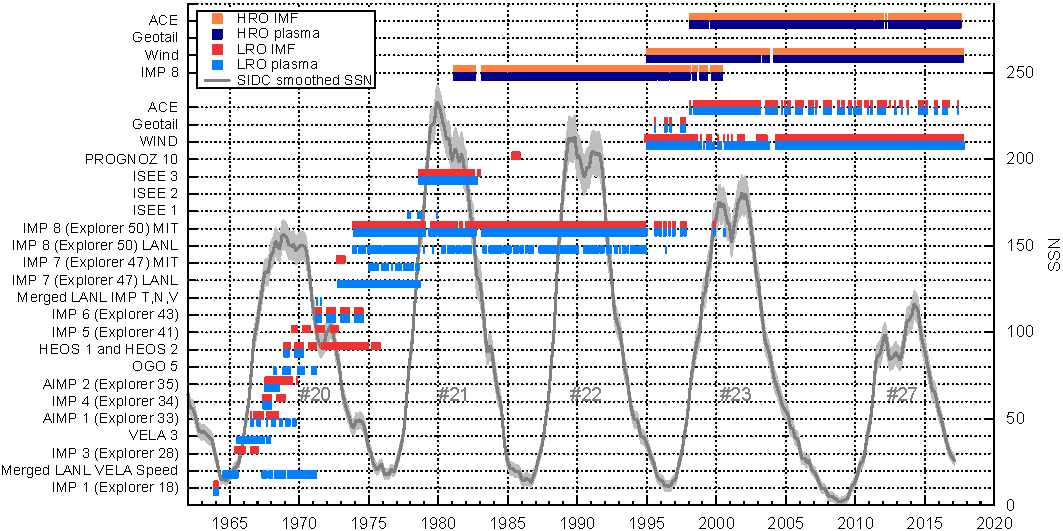
\includegraphics[width=\textwidth]{figures_of_mine/gnuplots/timeline_OMNI_SC_IDs.pdf}
	\caption[\lofimage{figures_of_mine/gnuplots/timeline_OMNI_SC_IDs.pdf}]
	{IMF and solar wind plasma data sources (spacecraft) for the high and the low resolution OMNI (HRO and LRO) data sets until the end of 2016. I plotted this figure using the spacecraft identifiers noted in the OMNIWeb Data Documentation\protect\footnotemark. The SIDC 13-month smoothed monthly SSN and the cycle number are plotted in the background.}
	\label{fig:timeline_OMNI_SC_IDs}
	\addtocontents{lof}{\smallskip\protect\center I created the figure myself.\medskip}
\end{figure}
\footnotetext{OMNIWeb Data Documentation: \urlfoot{https://omniweb.gsfc.nasa.gov/html/ow_data.html}}

The OMNI data set is being maintained at NASA's Space Physics Data Facility (SPDF), Goddard Space Flight Center (GSFC). Their OMNIWeb interface\footnote{GSFC OMNIWeb interface: \urlfoot{http://omniweb.gsfc.nasa.gov/}} and their Coordinated Data Analysis Web\footnote{GSFC CDAWeb interface: \urlfoot{http://cdaweb.gsfc.nasa.gov/}} (CDAWeb) provide the data -- the latter is where I obtained it.


Zhang2015 do with their data: ``The data have been lagged by 5~min to allow for propagation from the nose of bow shock to the magnetopause.''\\


\section{Helios probes}
\label{sec:helios_probes}
In order to observe solar wind in~situ within the inner heliosphere, the nearly identical solar probes Helios~1 and Helios~2, one is pictured in \autoref{fig:helios2}, were launched in December 1974 and January 1976 respectively.
\begin{figure}[htb]
	\begin{floatrow}
		\ffigbox[\FBwidth][]{
			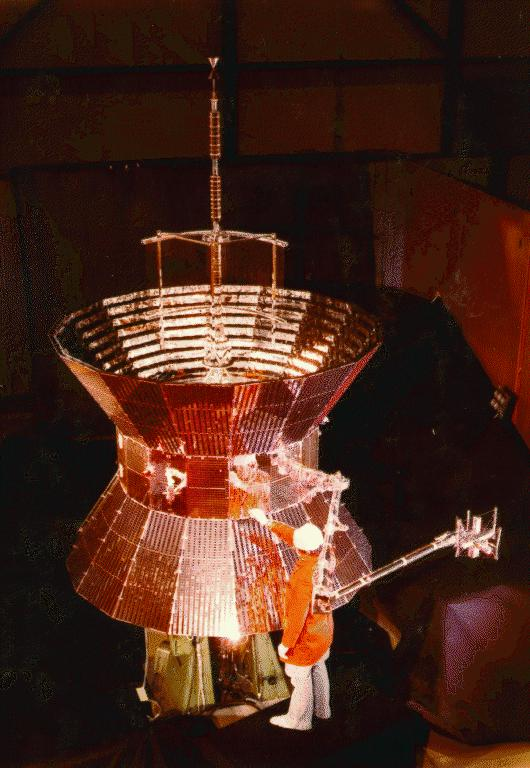
\includegraphics[width=0.3\textwidth]{figures_of_others/images/helios2.jpg}
		}{
			\caption[\lofimage{figures_of_others/images/helios2.jpg}Credit: \href{https://solarsystem.nasa.gov/missions/helios-1/in-depth/}{NASA/Max Planck Institute for Solar System Research}.]
			{One of the nearly identical twin Helios spacecraft\protect\footnotemark. Credit: \href{https://solarsystem.nasa.gov/missions/helios-1/in-depth/}{NASA/Max Planck Institute for Solar System Research}.}
			\label{fig:helios2}
			%source: https://solarsystem.nasa.gov/galleries/helios
			%alternative source: https://solarsystem.nasa.gov/missions/helios-1/in-depth/
			%NASA has no copyrights to its contents (NASA FOIA)
		}
		\ffigbox[\Xhsize]{
			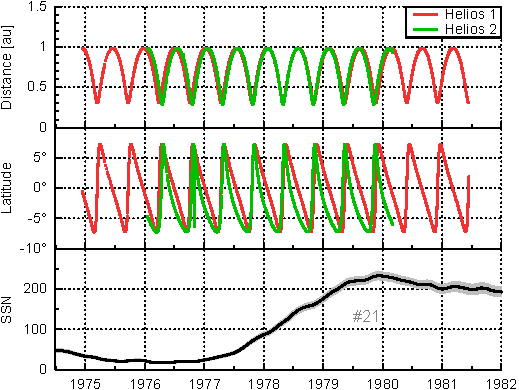
\includegraphics{figures_of_mine/gnuplots/Helios_r_b_ssn.pdf}
		}{
			\caption[\lofimage{figures_of_mine/gnuplots/Helios_r_b_ssn.pdf}]
			{Solar distance (top) and heliographic latitude (middle) of Helios~1 (red) and Helios~2 (green) with respect to their mission time. The trajectory data are from GSFC/SPDF and is plotted in HGI~coordinates. I plotted the SIDC 13-month smoothed monthly SSN and its cycle number in the bottom panel for orientation.}
			\label{fig:Helios_r_b_ssn}
		}
		\addtocontents{lof}{\smallskip\protect\center I created the figure myself.\medskip}
	\end{floatrow}
\end{figure}
\footnotetext{I was not able to find out which Helios spacecraft this is.}
Until today, these both probes were the only spacecraft that measured solar wind in~situ over large solar distance ranges with perihelia as close as \SI{0.31}{\au} and \SI{0.29}{\au} respectively. Their highly elliptical orbits in the ecliptic covered a solar distance range up to \SI{0.98}{\au}. Launched during solar cycle minimum, the data of both probes cover the rise to the maximum of solar cycle~21, that amounts to about 6.5~years of data at varying solar distances. I plotted the probes' solar distance and heliographic latitude with respect to their mission time and sunspot number for illustration in \autoref{fig:Helios_r_b_ssn}. The daily trajectory data are available from NASA's Space Physics Data Facility (SPDF) at the Goddard Space Flight Center (GSFC)\protect\footnote{SPDF Helios~1 trajectory data: \urlfoot{http://spdf.sci.gsfc.nasa.gov/pub/data/helios/helios1/traj/}} and are drawn in Heliographic Inertial (HGI) coordinates, see appendix \autoref{sec:coordinate_systems}. I also plotted the orbits of Helios~1 and Helios~2 in a solar equatorial plane view and in a solar polar plane view, see \autoref{fig:Helios12_orbits_ecliptic_polar}.
\begin{figure}[htb]
	\centering
	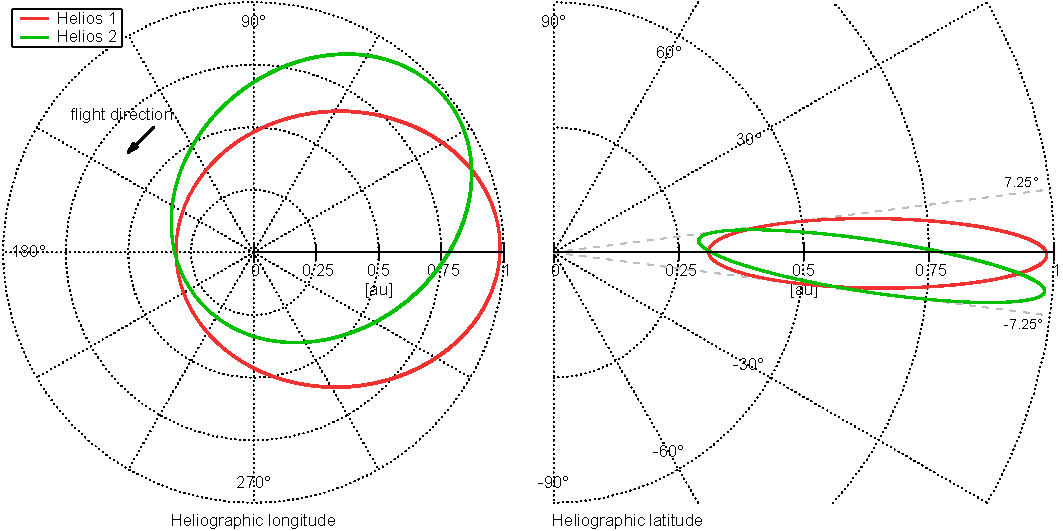
\includegraphics[width=\textwidth]{figures_of_mine/gnuplots/Helios12_orbits_ecliptic_polar.pdf}
	\caption[\lofimage{figures_of_mine/gnuplots/Helios12_orbits_ecliptic_polar.pdf}]
	{Orbits of the Helios~1 (red) and Helios~2 (green) spacecraft in the solar equatorial plane (left) and in the solar polar plane (right). I obtained the trajectory data from GSFC/SPDF and plotted the orbits in HGI~coordinates.}
	\label{fig:Helios12_orbits_ecliptic_polar}
	\addtocontents{lof}{\smallskip\protect\center I created the figure myself.\medskip}
\end{figure}

The scientific instruments carried by the spacecraft for measuring the magnetic field and solar wind plasma are two different Flux-gate Magnetometers and the Plasma Experiment Investigation. The data from the magnetometer and plasma instruments are merged into a data set with hourly resolution \citep{Rosenbauer1977}. In case of Helios~1 this data set includes about 12.5~orbits in the time range \mbox{1974-12-10} to \mbox{1981-06-14} and in case of Helios~2 about 8~orbits in the time range \mbox{1976-01-01} to \mbox{1980-03-04}. The Helios data is available via the GSFC/SPDF CDAWeb interface\footnote{GSFC CDAWeb interface: \urlfoot{http://cdaweb.gsfc.nasa.gov/}}.

The Helios~1 (Helios~2) magnetometer data coverage is about \SI{43}{\%} (\SI{54}{\%}) and amounts to 2.8~years (2.3~years) in total. The plasma data coverage is \SI{76}{\%} (\SI{92}{\%}) and amounts to 5.0~years (3.9~years) in total.\\

The Helios magnetic field and plasma data frequency over heliocentric distance and over heliographic latitude are plotted in \autoref{fig:helios_data_frequency}.\\
\begin{figure}[htb]
	\centering
	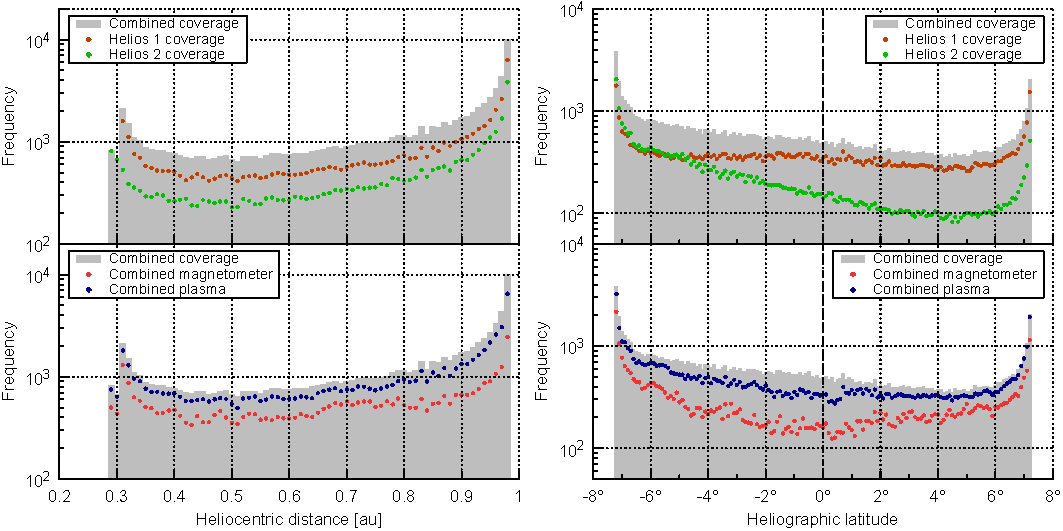
\includegraphics[width=\textwidth]{figures_of_mine/gnuplots/helios_data_frequency.pdf}
	\caption[\lofimage{figures_of_mine/gnuplots/helios_data_frequency.pdf}]
	{Helios data frequency over heliocentric distance with bins of \SI{0.01}{au} (left panels) and over heliographic latitude with bins of \SI{0.1}{\degree} (right panels). The frequency data is based on the hourly merged magnetometer and plasma data sets for Helios~1 and Helios~2. The top panels show the frequencies for Helios~1 and Helios~2 individually and the bottom panels those for the magnetometer and plasma data.}
	\label{fig:helios_data_frequency}
	\addtocontents{lof}{\smallskip\protect\center I created the figure myself.\medskip}
\end{figure}
\begin{figure}[htb]
	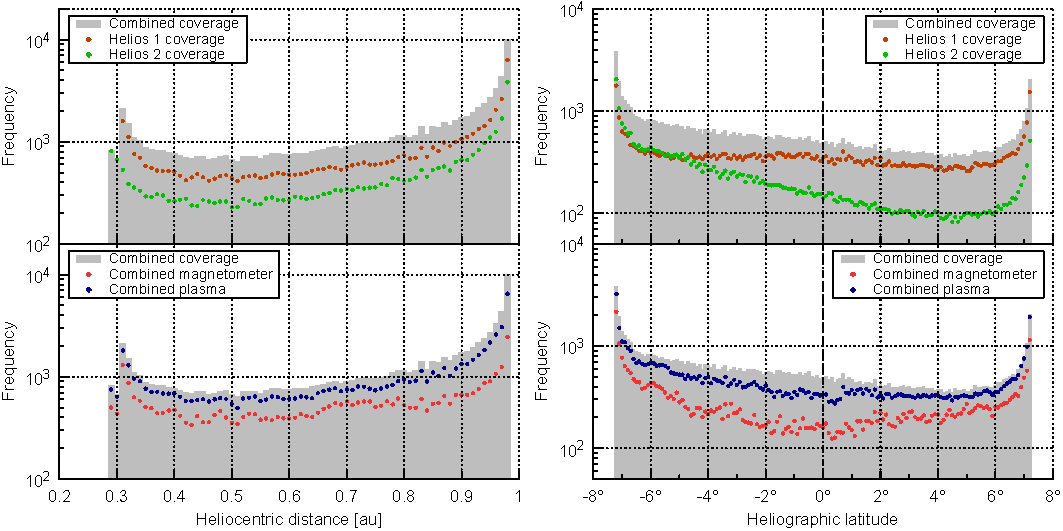
\includegraphics[width=\textwidth]{figures_of_mine/gnuplots/helios_data_frequency.pdf}
	\caption[\lofimage{figures_of_mine/gnuplots/helios_data_frequency.pdf}Remove later...]{}
\end{figure}


%see presi 1.07 Inside Helios-Origins and Evolution-Salem.ppt
%see book Schwenn1990 https://books.google.de/books?id=W1DuCAAAQBAJ&printsec=frontcover&dq=Physics+of+the+Inner+Heliosphere+I.+Large-Scale+Phenomena&hl=de&sa=X&redir_esc=y#v=onepage&q=Physics%20of%20the%20Inner%20Heliosphere%20I.%20Large-Scale%20Phenomena&f=false





% HELIOS~1 and 2 -- orbital Parameters:\\
% \url{http://spdf.sci.gsfc.nasa.gov/pub/data/helios/helios1/traj/}\\
% \url{http://spdf.sci.gsfc.nasa.gov/pub/data/helios/helios2/traj/}\\

% Helios hourly merged mag \& plasma data:\\
% HELIOS1\_COHO1HR\_MERGED\_MAG\_PLASMA\_2965.txt\\
% HELIOS2\_COHO1HR\_MERGED\_MAG\_PLASMA\_3096.txt\\
%\url{http://cdaweb.gsfc.nasa.gov}\\
% temporal coverage of merged data\\
% Helios 1: 1974-12-10 -- 1981-06-14\\
% Mag data availability: 42.6~\%\\
% Plasma \& orbit data availability: 76.4~\%\\
% Helios 2: 1976-01-01 -- 1980-03-04\\
% Mag data availability: 54.4~\%\\
% Plasma \& orbit data availability: 91.8~\%\\

